\hypertarget{02a_politika_uzayi}{%
\chapter{Faz 2A --- Politika uzayı: tek taraflı araçlar, iç vergiler ve dış rejim seçenekleri}\label{02a_politika_uzayi}}

\textbf{Durum:} Faz 2 / 9, birinci kısım (2A), 18 Ekim 2026. İkinci kısım: \belgebag{02b_secenekler_hukuk}{}{\kod{02b\_\allowbreak{}secenekler\_\allowbreak{}hukuk.\allowbreak{}md}}. Önceki faz: \belgebag{01_teshis}{}{\kod{01\_\allowbreak{}teshis.\allowbreak{}md}}. Defter: \belgebag{defter}{}{\kod{defter.\allowbreak{}md}}.

\textbf{Bu belge neden var?} Faz 1'e kullanıcının itirazı şuydu: yapılabileceklerin evreni keşfedilmedi. Örneğin GB'den çıkıp AB mallarına gümrük vergisi uygulamak ve yurt içinde üretilen mallarda ÖTV indirimi yapmak mümkün değil mi? İtiraz haklı. Faz 1, anlaşmasız çıkışı (S4) pasif bir senaryo olarak ele aldı: Türkiye AB mallarına MFN uygular, başka hiçbir şey yapmaz. Bu belge politika evrenini sistematik olarak tarıyor. Kapsam:

\begin{itemize}
\tightlist
\item
  kullanıcının önerisi: hukuki analiz, ekonomik eşdeğerlik, ürün grubu düzeyinde sayısallaştırma (§1);
\item
  tarife, iç vergi, sübvansiyon, kamu alımı, ticaret savunması, gümrük rejimleri, teknik mevzuat, dış anlaşmalar ve makro araçlardan oluşan araç evreni (§2);
\item
  Türkiye'nin kendi politika alanının sınırları: bağlı oranlar, yurt içi kabiliyet, koruma yapısı, gelir tabanı (§3);
\item
  anlaşmasız çıkışın Türkiye'nin kendi araçlarıyla yeniden hesaplanması, yani ``aktif S4'' (§4);
\item
  ihracat cephesinin sınırları (§5);
\item
  dış rejim seçenekleri (§6) ve zaman kritik eylemler (§7).
\end{itemize}

\textbf{Kanıt etiketleri:}

\begin{itemize}
\tightlist
\item
  \etiketV{}: doğrulanmış veri.
\item
  \etiketT{}: tahmin; yöntem ve P10--P50--P90 aralığı verilir.
\item
  \etiketD{}: doğrulanmalı.
\item
  \etiketH{}: hipotez veya uzman yargısı.
\end{itemize}

Her çıkarımın yanında Güven: Yüksek / Orta / Düşük düzeyi verilir. Tutarlar aksi belirtilmedikçe ABD doları ve cari fiyatlarla; ``mlr'' milyar, ``mn'' milyon, ``bp'' baz puandır (0,01 puan).

\textbf{Bu kısmın veri ve kodu.} Bütün sayılar aşağıdaki betiklerle yeniden üretilir; çıktılar \kod{veri/\allowbreak{}politika\_\allowbreak{}*.\allowbreak{}csv} dosyalarındadır.

\begingroup\gbtablo\small

\begin{longtable}[]{@{}
  >{\raggedright\arraybackslash}p{(\columnwidth - 4\tabcolsep) * \real{0.2559}}
  >{\raggedright\arraybackslash}p{(\columnwidth - 4\tabcolsep) * \real{0.3427}}
  >{\raggedright\arraybackslash}p{(\columnwidth - 4\tabcolsep) * \real{0.4014}}@{}}
\toprule\noalign{}
\begin{minipage}[b]{\linewidth}\raggedright
\textbf{Betik}
\end{minipage} & \begin{minipage}[b]{\linewidth}\raggedright
\textbf{İçerik}
\end{minipage} & \begin{minipage}[b]{\linewidth}\raggedright
\textbf{Ana kaynak}
\end{minipage} \\
\midrule\noalign{}
\endhead
\bottomrule\noalign{}
\endlastfoot
\kod{kod/\allowbreak{}f2a\_\allowbreak{}io\_\allowbreak{}fiyat.\allowbreak{}py} & Leontief fiyat modeli: tarife şokunun TÜFE'ye birinci tur etkisi & TÜİK 2023 girdi-çıktı tabloları (64 ürün) \\
\kod{kod/\allowbreak{}f2b\_\allowbreak{}tarife\_\allowbreak{}politikasi.\allowbreak{}py} & Tarife yapısı, BEC kullanım sınıfı, yurt içi kabiliyet ve ``girdide sıfır'' (P1) & BACI 2024, 2026 İthalat Rejimi Kararı, TÜİK PRODTR 2025, WITS BEC \\
\kod{kod/\allowbreak{}prodtr.\allowbreak{}py} & TÜİK Yıllık Sanayi Ürün İstatistikleri (CPA 2.2, 6 hane) & TÜİK Veri Portalı, bülten 58065 \\
\kod{kod/\allowbreak{}f2c0\_\allowbreak{}takas\_\allowbreak{}parametre.\allowbreak{}py}, \kod{kod/\allowbreak{}f2c\_\allowbreak{}vergi\_\allowbreak{}takasi.\allowbreak{}py} & Tarife + ÖTV/KDV takası, ürün grubu düzeyinde; dört tasarım & BACI 2024, PRODTR 2024, YSHİ 2024, ODMD 2025, GİB ÖTV listeleri, 2026 TÜFE ağırlıkları \\
\kod{kod/\allowbreak{}f2d\_\allowbreak{}s4\_\allowbreak{}net\_\allowbreak{}istihdam.\allowbreak{}py} & S4'te NACE sınıfı düzeyinde net istihdam: ihracat kaybı − ithal ikamesi & Faz 0 tarife duvarı, PRODTR, YSHİ \\
\kod{kod/\allowbreak{}f2e\_\allowbreak{}s4\_\allowbreak{}aktif.\allowbreak{}py} & Aktif S4 paketleri: İGV rejimi × P1 × vergi takası kapsamı & f2a, f2b; GİB 2025 gümrük vergisi tahsilatı \\
\end{longtable}

\endgroup

Hukuk, emsal ve AB tarafı bulguları Faz 2'nin dört araştırma ajanının birincil kaynak taramasından alındı:

\begin{itemize}
\tightlist
\item
  DTÖ hukuku;
\item
  Türkiye'nin ÖTV/KDV yapısı ve pazar verisi;
\item
  emsaller ve fiyat geçişkenliği;
\item
  AB hukuku ve çıkış mekaniği.
\end{itemize}

Kaynaklar sondadır; ham metinler ve çıkarılmış tablolar araştırma notlarında, \etiketV{} etiketli olanlar birincil metinden okunmuştur.

\begin{center}\rule{0.5\linewidth}{0.5pt}\end{center}

\hypertarget{02a_politika_uzayi-faz-2anux131n-12-ana-bulgusu}{%
\section{Faz 2A'nın 12 ana bulgusu}\label{02a_politika_uzayi-faz-2anux131n-12-ana-bulgusu}}

\begin{enumerate}
\def\labelenumi{\arabic{enumi}.}
\tightlist
\item
  \textbf{Gümrük birliğinden (GB) çıkınca AB mallarına gümrük vergisi konabilir; ÖTV indirimi ise yalnızca yerli ürüne yapılamaz.}

  \begin{itemize}
  \tightlist
  \item
    Tarife: MFN ilkesiyle ve bağlı oran içinde. Otomobilde Türkiye'nin cetvelindeki 18 satır \%19 ve \%20 ile bağlı; elektrikli otomobil \%20. Diğer içten yanmalı motorlu otomobil satırlarında bağlama yok (DS629 panel raporu, 28.7.2026).
  \item
    Yalnızca yerli ürüne ÖTV indirimi GATT md. III:2'nin ``kendiliğinden'' (per se) ihlalidir. III:8(b) bunu kurtarmaz; çünkü vergi indirimi ``sübvansiyon ödemesi'' sayılmaz (Brezilya--Vergilendirme, Temyiz Organı 2018, para. 5.92).
  \item
    Türkiye çok taraflı geçici temyiz düzenlemesine (MPIA) taraf değil. AB, ``boşluğa temyiz'' edilen bir panel raporuna dayanarak kendi Uygulama Tüzüğüyle misilleme yapabilir.
  \item
    \etiketV{} Güven: Yüksek.
  \end{itemize}
\item
  \textbf{Aynı amaç hukuken temiz bir biçimle elde edilebiliyor: tarife ile menşeden bağımsız ÖTV/KDV indiriminin takası (T-A).}

  \begin{itemize}
  \tightlist
  \item
    AB malına MFN tarifesi konur; aynı ürün grubunda bütün menşelere eşit ÖTV/KDV indirimi yapılır.
  \item
    Grubun fiyat endeksi sabit kalır; yerli ürün AB ürününe göre tarife kadar ucuzlar.
  \item
    Otomobilde (merkez tahmin):

    \begin{itemize}
    \tightlist
    \item
      ÖTV \%65'ten \%56,2'ye iner;
    \item
      AB otomobili \%4,1 pahalanır, yerli \%5,4 ucuzlar;
    \item
      yerli satış +\%23 (+\$1,2 mlr); istihdam +2,3 bin;
    \item
      net mali etki yılda −\$0,15 mlr.
    \end{itemize}
  \item
    Takas yapılmazsa otomobil tek başına TÜFE'ye +26 bp ekler.
  \item
    \etiketT{} Güven: Orta.
  \end{itemize}
\item
  \textbf{Önerinin ilk biçimi (T-0) yalnızca hukuka aykırı değil, pahalı da.}

  \begin{itemize}
  \tightlist
  \item
    Otomobil pazarının ancak \%22'si yerli. TÜFE'yi sabit tutmak için yerli otomobilde ÖTV'nin \%65'ten \%22,5'e inmesi gerekir. Bunun maliyeti yılda ≈\$3,0 mlr; on grupta ≈\$3,75 mlr. Takasta (T-A) maliyet ≈\$0,60 mlr.
  \item
    T-A'daki 8,8 puanlık indirim yalnızca yerliye uygulanırsa ucuz kalır, ama otomobilin TÜFE etkisinin ≈\%80'i yerinde durur.
  \item
    Yerli üreticiye doğrudan ödeme (T-B, III:8(b)) ekonomik olarak T-0 ile aynıdır. GATT md. III'e uygundur, ama Sübvansiyonlar ve Telafi Edici Önlemler Anlaşması (ASCM) kapsamında dava edilebilir.
  \item
    \etiketT{} Güven: Orta.
  \end{itemize}
\item
  \textbf{On ürün grubunda takasın bilançosu.}

  \begin{itemize}
  \tightlist
  \item
    Kapsam: otomobil, hafif ticari, beyaz eşya, küçük ev aletleri, TV, klima, kozmetik, giyim, ayakkabı, mobilya; TÜFE'nin \%17,4'ü.
  \item
    Sonuçlar önerilen İGV rejimi c2 altında (§4.1).
  \item
    Pasif S4: +47 bp TÜFE (P10--P90: 38--47), +\$1,65 mlr mali, +19 bin istihdam.
  \item
    Takas (T-A): 0 bp; −\$0,60 mlr (−0,71 ile +0,13); +31 bin istihdam (18--36 bin).
  \item
    Rejim c'de pasif S4 +35 bp; takasla −\$0,46 mlr ve +20 bin istihdam.
  \item
    \etiketT{} Güven: Orta.
  \end{itemize}
\item
  \textbf{Anlaşmasız çıkışın enflasyon sorunu Türkiye'nin kendi araçlarıyla çözülebiliyor.}

  \begin{itemize}
  \tightlist
  \item
    Pasif S4'te birinci tur TÜFE etkisi 78 bp (P10--P90: 59--98). Bunu ilk yılda 30 bp altına indiren dört paket bulundu.
  \item
    Önerilen paket (c2 + P1 + geniş takas):

    \begin{itemize}
    \tightlist
    \item
      İGV yalnızca yurt içi üretimi zayıf satırlarda kaldırılır;
    \item
      üretilmeyen girdilerde tarife sıfırlanır;
    \item
      imalat ürünlerinde menşeden bağımsız ÖTV/KDV takası yapılır.
    \end{itemize}
  \item
    Sonuç: TÜFE 3,3 bp (2,5--4,1). Tahsil edilebilir net mali etki GSYH'nin +\%0,05'i. Çin ve diğer kaynaklara karşı mevcut koruma korunuyor.
  \item
    \etiketT{} Güven: Orta.
  \end{itemize}
\item
  \textbf{İstihdam kısıtı aktif pakette daralıyor ama kapanmıyor; çekirdek giyim.}

  \begin{itemize}
  \tightlist
  \item
    S4'te imalatta net istihdam etkisi (σ = 5):

    \begin{itemize}
    \tightlist
    \item
      AB mallarına yalnızca MFN uygulanırsa −117 bin (P10--P90: −77 ile −165 bin);
    \item
      önerilen pakette (c2 + takas) ≈ −35 bin (≈ −11 ile −72 bin).
    \end{itemize}
  \item
    Farkın nedeni: İGV yurt içi üretimi güçlü satırlarda AB'ye de uygulanıyor; bu, ithal ikamesini ikiye katlıyor.
  \item
    Kaybın çekirdeği giyim: c2'de −58,7 bin (bölümün \%8,8'i). Diğer imalat bölümleri toplamda ≈ +11 bin.
  \item
    Giyimdeki kayıp AB pazarında oluşuyor. İç pazardaki hiçbir araç, AB'nin Türk ürünlerine uygulayacağı \%12'lik MFN'yi telafi etmiyor.
  \item
    \etiketT{} Güven: Orta.
  \end{itemize}
\item
  \textbf{İhracat tarafında yasal ve etkili bir tek taraflı araç yok.}

  \begin{itemize}
  \tightlist
  \item
    İhracat sübvansiyonu yasak.
  \item
    AB vergisini üretim desteğiyle telafi etmek yılda ≈\$38 mlr gerektirir (2028 GSYH'sinin \%1,8'i); AB bunu telafi edici vergiyle geri alır.
  \item
    Çıkışın ihracat cephesi bir anlaşmaya bağlı.
  \item
    \etiketT{} Güven: Orta.
  \end{itemize}
\item
  \textbf{Aktif S4, Türkiye'nin pazarlık gücünü artırıyor.}

  \begin{itemize}
  \tightlist
  \item
    AB'nin Türkiye'ye ihracatındaki kayıp (σ = 5, kısmi denge) rejime göre değişiyor:

    \begin{itemize}
    \tightlist
    \item
      yalnızca MFN uygulanırsa \$16,4 mlr;
    \item
      seçici rejimde (c) \$18,7 mlr;
    \item
      İGV kabiliyete duyarlı biçimde AB'ye de uygulanırsa (c2) \$28,5 mlr.
    \end{itemize}
  \item
    Türkiye, AB'nin üçüncü büyük yeni araç ihracat pazarı: 2025'te €18,8 mlr.
  \item
    Enflasyonu kendi araçlarıyla nötrleyebilen bir Türkiye için anlaşmasızlık daha az korkutucudur. Bu, anlaşmasız alternatifini (BATNA) güçlendirir.
  \item
    \etiketT{}/\etiketH{} Güven: Orta.
  \end{itemize}
\item
  \textbf{Çıkış hukuken AB'nin katılımını gerektiriyor.}

  \begin{itemize}
  \tightlist
  \item
    Ankara Anlaşması ve 1/95 sayılı Ortaklık Konseyi Kararı'nda fesih hükmü yok.
  \item
    En temiz teknik iki adımlıdır:

    \begin{itemize}
    \tightlist
    \item
      Ortaklık Konseyi'nin bir ``dondurma'' (standstill) kararı. AB tarafında nitelikli çoğunlukla alınabilir (ABİDA md. 207(4) ve 218(9)).
    \item
      AB'nin tek başına yetkili olduğu bir md. 207 anlaşması. Bu anlaşma GB hükümlerini ``etkisiz kılar'' (AB--Şili Geçici Ticaret Anlaşması md. 33.11 emsali).
    \end{itemize}
  \item
    Hasmane AB bu anlaşmayı önermeyebilir. Pazarlık, kozun kimde olduğuna bağlı.
  \item
    \etiketV{}/\etiketH{} Güven: Orta.
  \end{itemize}
\item
  \textbf{İki takvim için gerçekçilik.}

  \begin{itemize}
  \tightlist
  \item
    1.1.2028 için gerçekçi olan yalnızca çıkış kararı ve dondurma (geçiş dönemi). Ortaklık Konseyi kararı GB'yi kaldıramaz; GB'nin hukuken sona ermesi ITA'nın yürürlüğüyle olur.
  \item
    1.1.2029 için en fazla mal ağırlıklı bir serbest ticaret anlaşması (STA). Bunun için AB müzakere yetkisinin en geç 2027'nin üçüncü çeyreğinde verilmesi gerekir.
  \item
    Derin ve kapsamlı STA (DCFTA) 2030 sonrası bir projedir.
  \item
    \etiketH{} Güven: Orta.
  \end{itemize}
\item
  \textbf{Zaman kritik bir DTÖ adımı var: GATT md. XXVIII:5 çekincesi.}

  \begin{itemize}
  \tightlist
  \item
    Bağlı oranları 2027--2029'da yeniden müzakere edebilmek için Türkiye bu çekinceyi \textbf{31.12.2026'dan önce} bildirmeli.
  \item
    Bildirilmezse bu dönemde değişiklik ancak DTÖ'nün özel izniyle (XXVIII:4) yapılabilir. Olağan bir sonraki fırsat 1.1.2030.
  \item
    Bedeli: diğer üyeler de aynı dönemde Türkiye ile ilk müzakere ettikleri tavizleri değiştirebilir.
  \item
    DS629 panel raporu 27.10.2026'da DSB gündeminde. Güncelleme (Faz 2C): taraflar 16.10.2026'da kabul ya da temyiz süresinin 24.11.2026'ya uzatılmasını istedi (WT/DS629/6).
  \item
    \etiketV{} Güven: Yüksek.
  \end{itemize}
\item
  \textbf{Türkiye'nin mevcut iç vergi düzenlemelerinde, çıkıştan önce temizlenmesi gereken DTÖ riskleri var.} Bunlar çıkıştan sonra AB'nin ilk hedefleri olur:

  \begin{itemize}
  \tightlist
  \item
    Engelli araç alımındaki ÖTV istisnasının \%40 yerli katkı şartı.
  \item
    İhracat kazancına kurumlar vergisi indirimi (md. 32/7). Bu, ihracata bağlı sübvansiyon sayılabilir.
  \item
    Rakı ile diğer alkollü içkiler arasındaki maktu vergi farkı.
  \item
    Elektrikli araç ÖTV dilimlerinin 160 kW eşiği ve bununla ilgili açık ``yerli üretimi koruma'' beyanları.
  \item
    \etiketV{} Güven: Yüksek.
  \end{itemize}
\end{enumerate}

\begin{center}\rule{0.5\linewidth}{0.5pt}\end{center}

\hypertarget{02a_politika_uzayi-1-uxf6neri-ab-mallarux131na-guxfcmruxfck-vergisi--yurt-iuxe7inde-uxfcretilen-mallarda-uxf6tv-indirimi}{%
\section{1. Öneri: ``AB mallarına gümrük vergisi + yurt içinde üretilen mallarda ÖTV indirimi''}\label{02a_politika_uzayi-1-uxf6neri-ab-mallarux131na-guxfcmruxfck-vergisi--yurt-iuxe7inde-uxfcretilen-mallarda-uxf6tv-indirimi}}

\hypertarget{02a_politika_uzayi-11-kux131sa-cevap}{%
\subsection{1.1 Kısa cevap}\label{02a_politika_uzayi-11-kux131sa-cevap}}

\begin{enumerate}
\def\labelenumi{\arabic{enumi}.}
\item
  \textbf{Tarife kısmı mümkün.}

  \begin{itemize}
  \tightlist
  \item
    GB'den çıkınca Türkiye'nin AB'nin ortak gümrük tarifesine (OGT) bağlılığı biter. AB malları, STA'sı olmayan herkes gibi MFN oranını öder.
  \item
    Oran bağlı oranı aşamaz.
  \item
    AB'ye özel bir oran ancak bir STA veya GATT md. XXIV:5 kapsamında bir geçici anlaşmayla mümkündür.
  \end{itemize}
\item
  \textbf{ÖTV kısmı önerildiği biçimde mümkün değil.}

  \begin{itemize}
  \tightlist
  \item
    Yalnızca yurt içinde üretilen mallara ÖTV indirimi, ithal benzer ürünü yerliden daha ağır vergilemek demektir. Bu GATT md. III:2 birinci cümlenin doğrudan ihlalidir:

    \begin{itemize}
    \tightlist
    \item
      en küçük fark bile ihlaldir (Japonya--Alkollü İçkiler II, 1996);
    \item
      menşeye dayalı bir ayrım tek başına ihlal için yeter (Endonezya--Otomobil 1998, para. 14.113);
    \item
      ticaret etkisi veya asgari eşik savunması yoktur (Arjantin--Deri, 2001).
    \end{itemize}
  \item
    AB böyle bir uygulamayı dava eder ve kazanır.
  \end{itemize}
\item
  \textbf{Önerinin amacı ise hukuken temiz biçimde elde edilebilir.} Kullanıcının iki amacı var:

  \begin{itemize}
  \tightlist
  \item
    AB ürününe karşı yerli üreticiyi korumak;
  \item
    tarifenin enflasyonist etkisini nötrlemek.
  \end{itemize}

  Bu iki amaç, tarife + aynı ürün grubunda \textbf{bütün menşelere eşit} ÖTV/KDV indirimi takasıyla (T-A) birlikte sağlanır:

  \begin{itemize}
  \tightlist
  \item
    yerli ürün AB ürününe göre tarife kadar ucuzlar;
  \item
    grubun ortalama fiyatı değişmez;
  \item
    mali maliyet küçüktür, çünkü tarife geliri indirimi büyük ölçüde finanse eder.
  \end{itemize}
\item
  \textbf{Takas bir enflasyon kalkanıdır; ihracat çözümü değildir.} Yerli üreticiye iç pazarda avantaj verir. AB'nin Türk mallarına uygulayacağı MFN'yi ise değiştirmez. Otomotiv ihracatının \%79'u AB'ye gidiyor (Faz 1).
\end{enumerate}

\hypertarget{02a_politika_uzayi-12-hukuki-uxe7eruxe7eve}{%
\subsection{1.2 Hukuki çerçeve}\label{02a_politika_uzayi-12-hukuki-uxe7eruxe7eve}}

\begingroup\gbtablo\small

\begin{longtable}[]{@{}
  >{\raggedright\arraybackslash}p{(\columnwidth - 4\tabcolsep) * \real{0.1342}}
  >{\raggedright\arraybackslash}p{(\columnwidth - 4\tabcolsep) * \real{0.4449}}
  >{\raggedright\arraybackslash}p{(\columnwidth - 4\tabcolsep) * \real{0.4209}}@{}}
\toprule\noalign{}
\begin{minipage}[b]{\linewidth}\raggedright
\textbf{Kural}
\end{minipage} & \begin{minipage}[b]{\linewidth}\raggedright
\textbf{Özü}
\end{minipage} & \begin{minipage}[b]{\linewidth}\raggedright
\textbf{Öneriye uygulanışı}
\end{minipage} \\
\midrule\noalign{}
\endhead
\bottomrule\noalign{}
\endlastfoot
GATT III:2, birinci cümle & İthal ürün, benzer yerli üründen ``daha fazla'' iç vergiye tabi tutulamaz. Asgari eşik yok: ``en küçük fazlalık bile fazladır'' (Japonya--Alkollü İçkiler II, s. 23) & Yalnızca yerli araca ÖTV indirimi: \textbf{kendiliğinden ihlal} \\
GATT III:2, ikinci cümle ve Ek Not & Doğrudan rakip veya ikame ürünler ``korumaya yol açacak şekilde'' farklı vergilenemez. Ölçütler: tasarım, mimari ve ``açığa vuran yapı'' (revealing structure). Yalnızca nesnel olarak görünür amaç sayılır (Şili--Alkollü İçkiler, para. 71--72). Korumacı beyanlar delil olabilir (Meksika--Meşrubat, panel para. 8.91) & Görünüşte menşeden bağımsız ama yerli modelin özelliğine göre kesilmiş dilimler (ör. 160 kW eşiği): \textbf{fiilî ayrımcılık riski} \\
GATT III:4 & Satışı etkileyen düzenlemelerde ithal ürüne daha az elverişli muamele yasak; biçimsel eşitlik yetmez (Dominik Cumhuriyeti--Sigara) & İndirim yerli katkı, yerli tesiste üretim veya akreditasyon şartına bağlanırsa ihlal (Brezilya--Vergilendirme; Türkiye--Pirinç DS334) \\
GATT III:8(b) & Md. III, yalnızca yerli üreticilere sübvansiyon \textbf{ödenmesini} engellemez; iç vergi gelirinden finanse edilen ödemeler dahil & Kapsamı yalnızca kamu harcamasıdır; vergi muafiyeti veya indirimi kapsam dışı (Kanada--Süreli Yayınlar 1997, s. 33--34; Brezilya--Vergilendirme, para. 5.84, 5.92). Uygunluk ölçütü üretim faaliyeti olabilir, yerli girdi kullanımı olamaz (para. 5.93--5.95) \\
ASCM md. 1--3, 5--6, Kısım V & Vazgeçilen vergi geliri bir mali katkıdır. İhracata bağlı (3.1(a)) ve yerli girdiye bağlı (3.1(b)) sübvansiyonlar yasak. Sektöre özgü sübvansiyon dava edilebilir; sübvansiyonlu ülke pazarında ithalatın yerinden edilmesi ciddi zarardır (6.3(a)). İhracat pazarında telafi edici vergiye açık & III:8(b) ödemesi ASCM'den kaçamaz. AB hem Türkiye pazarındaki kaybı için dava açabilir (Endonezya--Otomobil'de ciddi zarar bulundu) hem de AB'ye giden Türk ürünlerine telafi edici vergi koyabilir \\
TRIMs md. 2 ve örnek liste & Yerli ürün satın alma veya kullanma (1(a)) ve ticaret dengeleme (1(b), 2(a)) şartları yasak; bir ``avantaj'' elde etmek için gerekiyorsa kapsam içinde (Endonezya--Otomobil, para. 14.88--14.91) & Takas ve III:8(b) desteği \textbf{koşulsuz} olmalı: yatırım, istihdam, Ar-Ge veya Türkiye'de üretim şartı olabilir; girdinin menşesi şartı olamaz \\
GATT I ve II:1 & MFN ve bağlı oran & AB'ye özel tarife STA olmadan mümkün değil. Bağlı oran aşılamaz (DS629: elektrikli araçlardaki ek vergiler II:1(b)'yi ihlal etti) \\
DTÖ uyuşmazlık çözümü (2026) & Temyiz Organı işlemiyor; 25.9.2026'da atama önerisi 100. kez engellendi. Türkiye MPIA'ya taraf değil & AB, Uygulama Tüzüğü 654/2014 md. 3(aa) ile, temyizi tamamlanamayan bir panel raporu sonrasında karşı önlem alabilir. Şikâyetten karşı önleme ≈2,5--3,5 yıl \etiketH{} \\
\end{longtable}

\endgroup

\emph{Kaynak ve etiketler:}

\begin{itemize}
\tightlist
\item
  \etiketV{} Antlaşma metinleri; DTÖ Analitik Endeksi (GATT md. III, ASCM md. 1--3, TRIMs md. 2).
\item
  DTÖ uyuşmazlık sayfaları: DS8/10/11, DS31, DS54/55/59/64, DS87/110, DS155, DS302, DS308, DS334, DS472/497, DS583, DS629.
\item
  DSB toplantısı, 25.9.2026; AB Tüzüğü 654/2014, 2021/167 ile değişik.
\item
  Güven: Yüksek.
\end{itemize}

\hypertarget{02a_politika_uzayi-13-emsaller-duxfcnyada-kim-ne-yaptux131-ne-oldu}{%
\subsection{1.3 Emsaller: dünyada kim ne yaptı, ne oldu?}\label{02a_politika_uzayi-13-emsaller-duxfcnyada-kim-ne-yaptux131-ne-oldu}}

\begingroup\gbtablo\footnotesize

\begin{longtable}[]{@{}
  >{\raggedright\arraybackslash}p{(\columnwidth - 8\tabcolsep) * \real{0.1646}}
  >{\raggedright\arraybackslash}p{(\columnwidth - 8\tabcolsep) * \real{0.2314}}
  >{\raggedright\arraybackslash}p{(\columnwidth - 8\tabcolsep) * \real{0.1857}}
  >{\raggedright\arraybackslash}p{(\columnwidth - 8\tabcolsep) * \real{0.2268}}
  >{\raggedright\arraybackslash}p{(\columnwidth - 8\tabcolsep) * \real{0.1915}}@{}}
\toprule\noalign{}
\begin{minipage}[b]{\linewidth}\raggedright
\textbf{Ülke ve önlem}
\end{minipage} & \begin{minipage}[b]{\linewidth}\raggedright
\textbf{Tasarım}
\end{minipage} & \begin{minipage}[b]{\linewidth}\raggedright
\textbf{Hukuki sonuç}
\end{minipage} & \begin{minipage}[b]{\linewidth}\raggedright
\textbf{Ölçülen etki}
\end{minipage} & \begin{minipage}[b]{\linewidth}\raggedright
\textbf{Ders}
\end{minipage} \\
\midrule\noalign{}
\endhead
\bottomrule\noalign{}
\endlastfoot
\textbf{Endonezya}, ``Millî Otomobil'' (1996) & Yerli içeriğe bağlı lüks satış vergisi ve gümrük muafiyeti & DS54/55/59/64 (1998): III:2, I, TRIMs 2.1 ihlali; ASCM'de ciddi zarar. 1999'da yeni politika & --- & Menşeye bağlı vergi ayrıcalığı ders kitabı ihlalidir \\
Endonezya, düşük maliyetli yeşil otomobil (LCGC) programı (2013--) ve 2021 indirimi & Motor hacmi, yakıt verimliliği ve fiyat ölçütü; yerli alım oranı \%60--70 şartı & Dava yok \etiketD{} & LCGC 2016'dan beri pazarın \textgreater\%20'si. 2021 indirimi: maliyet Rp4,6 trilyon, satış +\%67 (COVID tabanından) & Kısa süreli kriz önlemleri dava edilmedi, ama risk taşır \\
\textbf{Brezilya}, Inovar-Auto (2012--17) & Akredite yerli üreticiye 30 puanlık IPI (sanayi ürünleri vergisi) indirimi; ithalatçıya yılda 4.800 adetlik kota & DS472/497 (2019): III:2, III:4, I:1 ve TRIMs ihlali; III:8(b) savunması reddedildi & İthalatçıların satışı 199 binden (2011) ≈35 bine (2016) düştü. Brezilya'nın dünya üretimindeki payı kalıcı artmadı & Vergi indirimi ``sübvansiyon ödemesi'' sayılmaz \\
Brezilya, Rota 2030 (2018) ve MOVER (2024) & Aynı şartlar ve aynı IPI indirimleri ``Brezilya'da üretilen veya ithal edilen'' araçlara; MOVER'de itici güce, verimliliğe ve geri dönüştürülebilirliğe dayalı ``yeşil IPI'' & Rota 2030 DTÖ'ye uygun şablon. MOVER'in tam IPI muafiyeti Brezilya'da üretim şartı taşıyor: risk & MOVER Ar-Ge kredileri ≈R\$19 mlr & Menşeden bağımsız, teknolojiye dayalı vergi tasarımı mümkün \\
\textbf{Rusya}, geri dönüşüm harcı (2012--) & DTÖ üyeliğiyle tarife inerken ithal araçlara harç. Yerli üretici önce muaf; 2014'ten sonra yerli üretici de ödüyor ama federal sübvansiyonlarla telafi ediliyor & AB (DS462) ve Japonya (DS463): panel kuruldu ama hiç oluşturulmadı. USTR'ye göre fiilî ayrımcılık iddiası sürüyor & İthalat payı 2009'da \%48'den 2019'da \%15'e indi (rubledeki çöküş de etkili). Harç 2024--2025'te \%10--20 fiyat payına çıktı. Yerel montaj 2026'da satışların \%64'ü, ama yerli içerik sığ. 2026 bütçesinde gelir ≈RUB1,65 trilyon & ``Tek tip harç + yerli üreticiye telafi'' pratikte tarife gibi çalışır ve gelir getirir. Bedeli yüksek tüketici fiyatı ve gümrük birliği ortakları üzerinden sızıntı (Avrasya Ekonomik Birliği) \\
\textbf{Hindistan}, üretime bağlı teşvik (PLI, 2020--) & Artan satışın \%13--18'i oranında ödeme (otomotiv); en az \%50 yurt içi katma değer şartı & Çin'in açtığı DS642: panel 28.5.2026'da oluştu; sonuç bekleniyor & Haziran 2026'ya kadar ödeme ₹36.754 crore (bütçenin beşte birinden az). Telefon üretimi FY25'te +\%146; ithalat −\%77 & Üretime bağlı ödeme yaygın. Risk yurt içi katma değer şartında ve eşlik eden tarife artışlarında \\
\textbf{Çin}, yeni enerjili araç alım vergisi muafiyeti (2014--2027) & \%10 alım vergisinden muafiyet; kataloğa giren ithal modeller de yararlanıyor; 2026--27'de yarıya iniyor ve önceden ilan edildi & Menşeden bağımsız; dava yok & 2024--27 vergi harcaması ≈¥520 mlr & \textbf{Teknolojiye dayalı, menşeden bağımsız vergi indirimi hukuken sağlam.} Kademeli ve önceden ilan edilmiş çıkış \\
\textbf{Tayland}, elektrikli araç programları EV 3.0/3.5 (2022--27) & Alım sübvansiyonu ve ÖTV indirimi; ithalat vergisi indirimi karşılığında yerli üretim taahhüdü (1:1, sonra 1:2 ve 1:3); ithal batarya hücresi tavanı & Dava yok. Hücre tavanı ve ticaret dengeleme benzeri taahhüt III:4 ve TRIMs riski & 2025'e kadar 238 bin elektrikli araç; 43 üreticiden THB140 mlr yatırım; arz fazlası ve fiyat savaşı nedeniyle 2025'te şartlar gevşetildi & ``Şimdi ithal et, sonra üret'' hızlı yatırım çekti, ama tekrar tekrar gevşetme gerektirdi \\
\textbf{Arjantin}, Tierra del Fuego (2009--) & İthal elektroniğe yerli üretime göre çok daha yüksek iç vergi; bölge üretimi KDV'den muaf & Dava yok; menşeye dayalı iç vergi açık III:2 sorunu. Arjantin ticaret dengeleme şartlarından DS438'i kaybetti & Telefon pazarının \textgreater\%90'ı bölgeden; maliyet yılda ≈\$1,07 mlr & Menşeye göre değişen ÖTV gizli bir tarifedir; mali maliyeti yüksek ve kalıcı bir lobi yaratır \\
\textbf{ABD}, IRA temiz araç kredisi (30D, 2022--2025) & Kuzey Amerika'da son montaj ve kritik mineral oranı şartlı \$7.500 kredi & AB, Japonya ve Kore itiraz etti; Çin'in açtığı DS623'te kredi iddiaları, 30D kaldırıldıktan sonra (30.9.2025) düştü & --- & Üretim yerine bağlı tüketici kredisi müttefikleri kızdırdı; önce sulandırıldı, sonra kaldırıldı \\
\textbf{Türkiye}, ilaç yerelleştirmesi (2016--2024) & SGK geri ödemesinin yerelleştirmeye bağlanması & DS583 (DSU md. 25 tahkim kararı, 2022): III:4 ihlali; III:8(a) ve XX savunmaları reddedildi & --- & Türkiye'nin kendi dersi (temel ilke 8) \\
\textbf{Türkiye}, geçmiş ÖTV indirimleri (2009, 2017, 2018--19) & Otomobil, beyaz eşya ve mobilyada geçici indirimler & Hiçbirinde menşe şartı yok (CK 287 metni) & Kasım 2018: aylık TÜFE −\%1,44; otomobil fiyatı −\%13,6, mobilya −\%8,5, beyaz eşya −\%5,2. Geçişkenlik mobilyada ≈\%100, beyaz eşyada ≈\%83 & Menşeden bağımsız indirim Türkiye'de defalarca uygulandı; bu, takasın kurumsal altyapısıdır \\
\end{longtable}

\endgroup

\emph{Kaynak ve etiketler:}

\begin{itemize}
\tightlist
\item
  \etiketV{} DTÖ uyuşmazlık sayfaları: DS54, DS462/463, DS472/497, DS438, DS583, DS623, DS642.
\item
  USTR 2022 ve 2025 Rusya raporları; TCMB Kasım 2018 fiyat gelişmeleri raporu; CK 287 (RG 31.10.2018 mük.).
\item
  \etiketD{} Rusya, Endonezya, Tayland, Arjantin ve Hindistan'ın ölçülen etkilerinde basın ve ikincil kaynaklar kullanıldı.
\item
  Güven: Orta.
\end{itemize}

\hypertarget{02a_politika_uzayi-14-ekonomik-eux15fdeux11ferlik-ve-tasarux131m-seuxe7enekleri}{%
\subsection{1.4 Ekonomik eşdeğerlik ve tasarım seçenekleri}\label{02a_politika_uzayi-14-ekonomik-eux15fdeux11ferlik-ve-tasarux131m-seuxe7enekleri}}

Bir ithalat tarifesi ekonomik olarak iki aracın toplamıdır: yerli üreticiye \textbf{üretim sübvansiyonu} ve tüketiciye \textbf{tüketim vergisi} (Bhagwati--Ramaswami 1963).

\begin{itemize}
\tightlist
\item
  Tarife ile aynı ürün grubundaki menşeden bağımsız ÖTV indirimi birlikte uygulanırsa tüketim vergisi kısmı nötrlenir.
\item
  Geriye tarife geliriyle finanse edilen bir üretim sübvansiyonu kalır. Yerli üretici AB ürününe göre tarife kadar fiyat avantajı kazanır; tüketici ortalamada aynı fiyatı öder.
\item
  Hedefleme ilkesine göre amaç yerli üretimse en verimli araç doğrudan üretim sübvansiyonudur. Ancak bu araç bütçeden finanse edilir ve ASCM'ye tabidir. Takas, tarife gelirini kullandığı için mali olarak neredeyse kendi kendini finanse eder.
\end{itemize}

\begingroup\gbtablo\footnotesize

\begin{longtable}[]{@{}
  >{\raggedright\arraybackslash}p{(\columnwidth - 12\tabcolsep) * \real{0.1628}}
  >{\raggedright\arraybackslash}p{(\columnwidth - 12\tabcolsep) * \real{0.2139}}
  >{\raggedright\arraybackslash}p{(\columnwidth - 12\tabcolsep) * \real{0.1149}}
  >{\raggedright\arraybackslash}p{(\columnwidth - 12\tabcolsep) * \real{0.1280}}
  >{\raggedright\arraybackslash}p{(\columnwidth - 12\tabcolsep) * \real{0.1210}}
  >{\raggedright\arraybackslash}p{(\columnwidth - 12\tabcolsep) * \real{0.1356}}
  >{\raggedright\arraybackslash}p{(\columnwidth - 12\tabcolsep) * \real{0.1237}}@{}}
\toprule\noalign{}
\begin{minipage}[b]{\linewidth}\raggedright
\textbf{Tasarım}
\end{minipage} & \begin{minipage}[b]{\linewidth}\raggedright
\textbf{Yerli ürünün AB ürününe göre fiyat avantajı}
\end{minipage} & \begin{minipage}[b]{\linewidth}\raggedright
\textbf{STA ortağının (Kore, İngiltere, Fas) ürününe göre}
\end{minipage} & \begin{minipage}[b]{\linewidth}\raggedright
\textbf{Grubun TÜFE'si}
\end{minipage} & \begin{minipage}[b]{\linewidth}\raggedright
\textbf{Mali}
\end{minipage} & \begin{minipage}[b]{\linewidth}\raggedright
\textbf{DTÖ riski}
\end{minipage} & \begin{minipage}[b]{\linewidth}\raggedright
\textbf{AB'nin misilleme riski}
\end{minipage} \\
\midrule\noalign{}
\endhead
\bottomrule\noalign{}
\endlastfoot
\textbf{T-0} Tarife + yalnızca yerli ürüne ÖTV indirimi (önerinin ilk biçimi) & Tarife + ÖTV farkı (otomobilde \%48) & ÖTV farkı & Sabitlenirse çok pahalı; ucuz tutulursa artar & Yüksek negatif (TÜFE sabitlenirse) & \textbf{Yüksek}: III:2 kendiliğinden ihlal; şarta bağlanırsa III:4, TRIMs ve ASCM 3.1(b) & Yüksek (md. 3(aa); MPIA yok) \\
\textbf{T-A} Tarife + menşeden bağımsız ÖTV/KDV indirimi (takas) & Tarife kadar (otomobilde \%10) & Yok & Sabit (tasarım gereği) & ≈ Nötr & \textbf{Düşük} & Düşük--orta (bağlı oran aşılırsa XXVIII dengelemesi) \\
\textbf{T-B} Tek tip ÖTV + yerli üreticiye III:8(b) birim ödemesi & Ödeme kadar & Ödeme kadar & Sabitlenebilir & Yüksek negatif (bütçeden) & Düşük (GATT); orta (ASCM: ciddi zarar davası) & Düşük--orta; telafi edici vergi riski orta--yüksek \\
\textbf{T-C} ÖTV'nin nesnel ölçütlerle yeniden yapılandırılması (CO₂, verimlilik, boyut) & Ölçütün yerli modelle örtüşmesine bağlı & Aynı & ± & ± & Düşük--orta; eşikler yerli modele göre kesilirse orta & Düşük \\
\textbf{T-D} Kamu alımında yerli malı fiyat avantajı & \%15'e kadar (yalnızca gerçek kamu alımında) & Aynı & Etkisiz & Hafif negatif & Düşük (Türkiye Hükûmet Alımları Anlaşması'na taraf değil, gözlemci) & Orta (AB'nin Uluslararası Kamu Alımı Aracı) \\
\textbf{T-E} Ticaret savunması (anti-damping, telafi edici vergi) & Dampingli/sübvansiyonlu ithalata karşı & --- & Hafif + & + & Düşük (kanıta dayalıysa) & Düşük--orta \\
\textbf{T-F} Korunma önlemi & Herkese karşı & Herkese karşı & + & + & Orta--yüksek (çıkışta AB ithalatı artmaz, azalır; ``ithalat artışı'' koşulu sağlanamaz) & Orta--yüksek (md. 8.2 karşı önlem) \\
\end{longtable}

\endgroup

\emph{Kaynak ve etiketler:} \etiketV{} hukuki değerlendirme DTÖ araştırma notunun sıralı tasarım tablosuna dayanıyor. \etiketT{} sayılar §1.5'ten. Güven: Orta--Yüksek.

\textbf{T-0 ile T-A arasındaki fark, sanıldığı gibi yalnızca hukuki değil.}

\begin{itemize}
\tightlist
\item
  T-0'da yerli ürüne yapılan ÖTV indirimi küçük bir tabana uygulanır: otomobil pazarının \%22'si.
\item
  Pazarın geri kalanında, yani AB ve diğer ithal ürünlerde fiyat tarife kadar artar.
\item
  Bu nedenle T-0 grubun fiyatını ya sabitleyemez ya da sabitlemek için yerli üründe çok derin bir indirim gerektirir. Derin indirim yerliye \%48'lik bir fiyat avantajı verir; bu, hukuka aykırılığın büyüklüğünün de ölçüsüdür.
\item
  T-A ise indirimi bütün pazara yayar. Gereken indirim küçüktür ve tarife geliri onu finanse eder.
\end{itemize}

\hypertarget{02a_politika_uzayi-15-uxfcruxfcn-grubu-duxfczeyinde-sonuuxe7lar}{%
\subsection{1.5 Ürün grubu düzeyinde sonuçlar}\label{02a_politika_uzayi-15-uxfcruxfcn-grubu-duxfczeyinde-sonuuxe7lar}}

\textbf{Model} (\kod{kod/\allowbreak{}f2c\_\allowbreak{}vergi\_\allowbreak{}takasi.\allowbreak{}py}):

\begin{itemize}
\tightlist
\item
  On ürün grubu; kaynaklar yerli, AB, STA ortakları ve diğerleri.
\item
  Armington CES talep sistemi:

  \begin{itemize}
  \tightlist
  \item
    ikame esnekliği σ ∈ \{2, 4, 6\};
  \item
    grup talebinin fiyat esnekliği η ∈ \{0,5; 1; 1,5\};
  \item
    tarifenin fiyata geçişkenliği ρ ∈ \{0,8; 1\}.
  \end{itemize}
\item
  S4 tarife rejimi: önerilen c2 (§4.1). İGV, AB'nin baskın ve yurt içi kabiliyetin zayıf olduğu satırlarda herkes için kalkar; diğer satırlarda AB'ye de uygulanır. Rejim c sonuçları karşılaştırma için verildi.
\item
  Takas kuralı: grubun \textbf{ölçülen} fiyat endeksi (Laspeyres; TÜFE ağırlıkları yıl içinde sabit) değişmez. Refah açısından tam fiyat endeksi (CES) ayrıca raporlandı.
\item
  Merkez tahmin σ = 4, η = 1, ρ = 1. Aralık, 18 parametre bileşiminin P10--P90'ı.
\end{itemize}

\textbf{Veri:}

\begin{itemize}
\tightlist
\item
  İthalat ve ihracat: BACI 2024.
\item
  Yerli iç satış: PRODTR 2024 (az sayıda üreticili gruplarda), YSHİ 2024 (parçalı sektörlerde), 2023 girdi-çıktı tablosu (giyimde) ve ODMD 2025 (otomobil ve hafif ticari).
\item
  ÖTV ve KDV: GİB listeleri, 2026.
\item
  TÜFE ağırlıkları: 2026, COICOP 2018.
\end{itemize}

\begin{landscape}

\textbf{Tablo 1.5a --- Takas (T-A) ve pasif S4, ürün grubu başına (rejim c2, merkez)}

\nopagebreak[4]

\begingroup\gbtablo\footnotesize

\begin{longtable}[]{@{}
  >{\raggedright\arraybackslash}p{(\columnwidth - 18\tabcolsep) * \real{0.0779}}
  >{\raggedleft\arraybackslash}p{(\columnwidth - 18\tabcolsep) * \real{0.0869}}
  >{\raggedleft\arraybackslash}p{(\columnwidth - 18\tabcolsep) * \real{0.0545}}
  >{\raggedleft\arraybackslash}p{(\columnwidth - 18\tabcolsep) * \real{0.1388}}
  >{\raggedleft\arraybackslash}p{(\columnwidth - 18\tabcolsep) * \real{0.0860}}
  >{\raggedleft\arraybackslash}p{(\columnwidth - 18\tabcolsep) * \real{0.1104}}
  >{\raggedleft\arraybackslash}p{(\columnwidth - 18\tabcolsep) * \real{0.1269}}
  >{\raggedleft\arraybackslash}p{(\columnwidth - 18\tabcolsep) * \real{0.1020}}
  >{\raggedleft\arraybackslash}p{(\columnwidth - 18\tabcolsep) * \real{0.1213}}
  >{\raggedleft\arraybackslash}p{(\columnwidth - 18\tabcolsep) * \real{0.0953}}@{}}
\toprule\noalign{}
\begin{minipage}[b]{\linewidth}\raggedright
\textbf{Grup}
\end{minipage} & \begin{minipage}[b]{\linewidth}\raggedleft
\textbf{TÜFE ağırlığı (\%)}
\end{minipage} & \begin{minipage}[b]{\linewidth}\raggedleft
\textbf{Yerli pay}
\end{minipage} & \begin{minipage}[b]{\linewidth}\raggedleft
\textbf{ÖTV/KDV: bugün → takasla}
\end{minipage} & \begin{minipage}[b]{\linewidth}\raggedleft
\textbf{Pasif S4: grup fiyatı}
\end{minipage} & \begin{minipage}[b]{\linewidth}\raggedleft
\textbf{Pasif S4: TÜFE katkısı (bp)}
\end{minipage} & \begin{minipage}[b]{\linewidth}\raggedleft
\textbf{Takasla AB ürünü / yerli ürün fiyatı}
\end{minipage} & \begin{minipage}[b]{\linewidth}\raggedleft
\textbf{Takasla yerli satış (\$ mn)}
\end{minipage} & \begin{minipage}[b]{\linewidth}\raggedleft
\textbf{Takasla istihdam}
\end{minipage} & \begin{minipage}[b]{\linewidth}\raggedleft
\textbf{Takasla net mali (\$ mn)}
\end{minipage} \\
\midrule\noalign{}
\endhead
\bottomrule\noalign{}
\endlastfoot
Binek otomobil & 4,59 & \%22 & ÖTV \%65 → \%56,2 & +\%5,7 & 26,0 & +\%4,1 / −\%5,4 & +1.189 & +2.300 & −153 \\
Hafif ticari & 0 & \%22 & ÖTV \%6 → \%0 (yetmiyor; kalan +\%1,5) & +\%7,6 & 0 & +\%7,1 / −\%5,7 & +161 & +312 & +7 \\
Beyaz eşya & 1,06 & \%86 & ÖTV \%6,7 → \%5,7 & +\%1,0 & 1,0 & +\%9,8 / −\%1,0 & +96 & +491 & −9 \\
Küçük ev aletleri & 0,19 & \%33 & ÖTV \%6,7 → \%3,1 & +\%3,5 & 0,7 & +\%16,9 / −\%3,4 & +73 & +374 & −10 \\
TV & 0,26 & \%74 & ÖTV \%6,7 → \%6,0 & +\%0,7 & 0,2 & +\%13,2 / −\%0,7 & +15 & +80 & −2 \\
Klima & 0,16 & \%77 & ÖTV değişmez & +\%0,0 & 0,0 & +\%2,0 / 0 & +2 & +17 & 0 \\
Kozmetik & 0,92 & \%39 & ÖTV \%20 → \%13,4 & +\%5,8 & 5,3 & +\%8,2 / −\%5,5 & +159 & +1.353 & −27 \\
Giyim & 6,51 & \%87 & KDV \%10 → \%8,7 & +\%1,2 & 7,7 & +\%47,5 / −\%1,2 & +949 & +20.360 & −319 \\
Ayakkabı & 1,11 & \%45 & KDV \%10 → \%5,6 & +\%4,1 & 4,6 & +\%43,7 / −\%4,0 & +202 & +3.368 & −63 \\
Mobilya & 2,62 & \%91 & KDV \%10 → \%9,3 & +\%0,6 & 1,7 & +\%15,8 / −\%0,6 & +137 & +2.792 & −19 \\
\textbf{Toplam} & \textbf{17,41} & & & & \textbf{47,2 (38--47)} & & \textbf{+2.984} & \textbf{+31.447 (17.708--35.726)} & \textbf{−596 (−706 ile +127)} \\
\end{longtable}

\endgroup

\end{landscape}

\emph{Kaynak ve etiketler:}

\begin{itemize}
\tightlist
\item
  \etiketT{} \kod{veri/\allowbreak{}politika\_\allowbreak{}takas\_\allowbreak{}ozet.\allowbreak{}csv}, \kod{veri/\allowbreak{}politika\_\allowbreak{}takas\_\allowbreak{}parametre.\allowbreak{}csv}.
\item
  Yerli payın kaynağı: otomobil ve hafif ticaride ODMD 2025 adet payı × OSD ihracat birim değeri; beyaz eşya, küçük ev aletleri, TV, klima ve kozmetikte PRODTR 2024; ayakkabı ve mobilyada YSHİ 2024; giyimde 2023 girdi-çıktı tablosundaki hanehalkı yurt içi payı.
\item
  Üç yöntem arasındaki fark parametre dosyasında raporlandı. Otomobilde I-O payı \%39, YSHİ payı \%54; ikisi de hafif ticari ve parça üretimini karıştırıyor.
\item
  Rejim c'de toplamlar: pasif S4 +34,7 bp; takasla −\$462 mn net mali ve +20.066 istihdam.
\item
  Güven: Orta.
\end{itemize}

\textbf{Okuma.}

\begin{itemize}
\tightlist
\item
  \textbf{Kozmetik ve mobilyada rejim seçimi işaret değiştiriyor.}

  \begin{itemize}
  \tightlist
  \item
    Rejim c'de AB'nin baskın olduğu satırlarda İGV herkes için kalkıyordu. Fiyatlar düşüyor, yerli üretici kaybediyordu: mobilyada −2,4 bin, kozmetikte −0,4 bin istihdam.
  \item
    c2'de yurt içi üretimi güçlü satırlarda İGV korunuyor. AB ve diğer ithal ürünler pahalanıyor, takas bu artışı ÖTV/KDV indirimiyle siliyor. Yerli üretici kazanıyor: mobilyada +2,8 bin, kozmetikte +1,4 bin.
  \end{itemize}
\item
  \textbf{Giyim ve ayakkabıda AB ürününün fiyatı \%44--48 artıyor}, çünkü İGV AB'ye de uygulanıyor.

  \begin{itemize}
  \tightlist
  \item
    AB'nin iç pazardaki payı küçük (\%2--8). TÜFE etkisini küçük bir KDV indirimi siliyor.
  \item
    Bu iki grup takasın istihdam getirisinin ≈\%75'ini oluşturuyor.
  \end{itemize}
\item
  \textbf{Küçük ev aletlerinde yerli pay düşük (\%33).} TÜFE'yi sabit tutmak için ÖTV'nin \%6,7'den \%3,1'e inmesi gerekiyor.
\end{itemize}

\Needspace{7\baselineskip}

\textbf{Tablo 1.5b --- Otomobilde dört tasarım (merkez; aralık P10--P90)}

\nopagebreak[4]

\begingroup\gbtablo\footnotesize

\begin{longtable}[]{@{}
  >{\raggedright\arraybackslash}p{(\columnwidth - 8\tabcolsep) * \real{0.2444}}
  >{\raggedleft\arraybackslash}p{(\columnwidth - 8\tabcolsep) * \real{0.0933}}
  >{\raggedleft\arraybackslash}p{(\columnwidth - 8\tabcolsep) * \real{0.1610}}
  >{\raggedleft\arraybackslash}p{(\columnwidth - 8\tabcolsep) * \real{0.2142}}
  >{\raggedleft\arraybackslash}p{(\columnwidth - 8\tabcolsep) * \real{0.2871}}@{}}
\toprule\noalign{}
\begin{minipage}[b]{\linewidth}\raggedright
\end{minipage} & \begin{minipage}[b]{\linewidth}\raggedleft
\textbf{Pasif S4}
\end{minipage} & \begin{minipage}[b]{\linewidth}\raggedleft
\textbf{T-A takas}
\end{minipage} & \begin{minipage}[b]{\linewidth}\raggedleft
\textbf{T-0 yalnızca yerliye indirim}
\end{minipage} & \begin{minipage}[b]{\linewidth}\raggedleft
\textbf{T-B III:8(b) ödemesi}
\end{minipage} \\
\midrule\noalign{}
\endhead
\bottomrule\noalign{}
\endlastfoot
ÖTV (ithal / yerli) & \%65 / \%65 & \%56,2 / \%56,2 & \%65 / \textbf{\%22,5} & \%65 / \%65 \\
Yerli üreticiye birim ödeme & --- & --- & --- & Üretici fiyatının \%25,8'i \\
AB otomobilinin fiyatı & +\%10,0 & +\%4,1 & +\%10,0 & +\%10,0 \\
Yerli otomobilin fiyatı & 0 & −\%5,4 & −\%25,8 & −\%25,8 \\
Yerlinin AB'ye göre fiyat avantajı & \%10 & \%10 & \textbf{\%48} & \textbf{\%48} \\
Yerli satış hacmi & +\%16 & +\%23 (+9 ile +34) & +\%180 (+57 ile +276) & +\%180 \\
Otomobilin TÜFE katkısı & +26,0 bp & 0 & 0 & 0 \\
Net mali etki (\$ mn/yıl) & +1.102 & \textbf{−153} (−212 ile +193) & \textbf{−2.992} (−4.194 ile −664) & \textbf{−2.992} \\
İstihdam & +1.641 & +2.300 & +17.977 & +17.977 \\
DTÖ & Uyumlu & Uyumlu & \textbf{Aykırı} & Uyumlu (GATT); ASCM'de dava edilebilir \\
\end{longtable}

\endgroup

\emph{Kaynak:} \etiketT{} aynı model. T-0 ve T-B'de yerli satıştaki +\%180 bir kapasite sınırına çarpar: yerli üretimin iç satışı 323 bin adetten ≈900 bin adede çıkmak zorunda kalır. Bu, ihracattan iç pazara kaydırma olmadan mümkün değildir. Sayı bir üst sınır olarak okunmalı. Güven: Orta.

\textbf{Otomobilde bir ara yol: T-0'da indirim T-A ile aynı tutulursa.} ÖTV yalnızca yerli otomobilde 8,8 puan indirilir.

\begin{itemize}
\tightlist
\item
  Yerli fiyat −\%5,4, AB fiyatı +\%10 olur.
\item
  Grup fiyatı +\%4,5 artar; TÜFE katkısı ≈+20,5 bp, yani pasif S4'ün ≈\%80'i.
\item
  Mali maliyet küçük kalır (≈+\$0,7 mlr net), ama hukuka aykırılık aynıdır.
\item
  Kısacası T-0 ya pahalıdır ya da enflasyonu durdurmaz. \etiketT{}
\end{itemize}

\Needspace{7\baselineskip}

\textbf{Tablo 1.5c --- On grubun toplamı, dört tasarım (rejim c2; merkez; aralık P10--P90)}

\nopagebreak[4]

\begingroup\gbtablo\footnotesize

\begin{longtable}[]{@{}
  >{\raggedright\arraybackslash}p{(\columnwidth - 8\tabcolsep) * \real{0.2112}}
  >{\raggedleft\arraybackslash}p{(\columnwidth - 8\tabcolsep) * \real{0.1867}}
  >{\raggedleft\arraybackslash}p{(\columnwidth - 8\tabcolsep) * \real{0.1963}}
  >{\raggedleft\arraybackslash}p{(\columnwidth - 8\tabcolsep) * \real{0.1970}}
  >{\raggedleft\arraybackslash}p{(\columnwidth - 8\tabcolsep) * \real{0.2087}}@{}}
\toprule\noalign{}
\begin{minipage}[b]{\linewidth}\raggedright
\end{minipage} & \begin{minipage}[b]{\linewidth}\raggedleft
\textbf{Pasif S4}
\end{minipage} & \begin{minipage}[b]{\linewidth}\raggedleft
\textbf{T-A takas}
\end{minipage} & \begin{minipage}[b]{\linewidth}\raggedleft
\textbf{T-0}
\end{minipage} & \begin{minipage}[b]{\linewidth}\raggedleft
\textbf{T-B}
\end{minipage} \\
\midrule\noalign{}
\endhead
\bottomrule\noalign{}
\endlastfoot
TÜFE katkısı (bp) & +47,2 (38--47) & 0 & ≈0 (+0,3) & 0 \\
Gümrük geliri (\$ mn) & +1.645 & +1.796 & +1.073 & +994 \\
ÖTV + KDV (\$ mn) & 0 & −2.393 & −4.824 & 0 \\
Yerli üreticiye ödeme (\$ mn) & --- & --- & --- & −5.583 \\
\textbf{Net mali (\$ mn)} & \textbf{+1.645} (1.014--2.429) & \textbf{−596} (−706 ile +127) & \textbf{−3.751} (−5.213 ile −777) & \textbf{−4.589} (−6.383 ile −1.081) \\
Yerli satış (\$ mn) & +1.963 & +2.984 & +12.433 & +13.929 \\
İstihdam & +19.074 (6.300--24.661) & +31.447 (17.708--35.726) & +64.269 (29.441--83.339) & +67.576 (30.382--87.857) \\
\end{longtable}

\endgroup

\emph{Kaynak:} \etiketT{} \kod{veri/\allowbreak{}politika\_\allowbreak{}takas\_\allowbreak{}ozet.\allowbreak{}csv}. Rejim c için aynı tablo dosyada (pasif +34,7 bp; T-A −\$462 mn; T-0 −\$3.447 mn; T-B −\$4.217 mn). Güven: Orta.

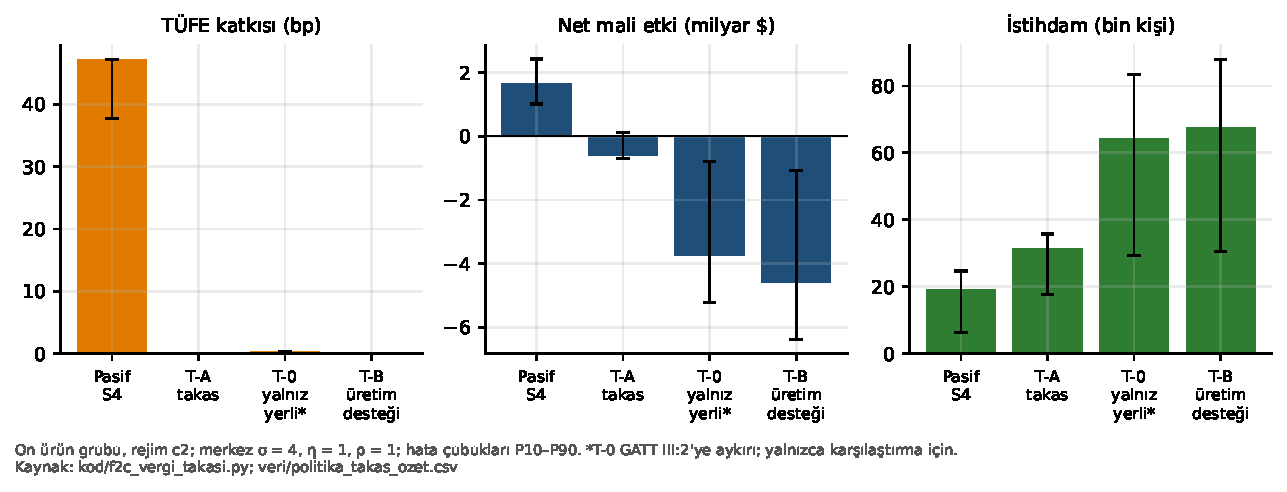
\includegraphics[width=1\textwidth,height=\textheight]{sekiller/f2_takas_tasarim.pdf}

\emph{Şekil 2A.1 --- Vergi takası: dört tasarımın TÜFE, net mali ve istihdam etkisi (on ürün grubu, rejim c2; P10--P90)}

\textbf{Okuma.}

\begin{enumerate}
\def\labelenumi{\arabic{enumi}.}
\tightlist
\item
  TÜFE'yi sabitleyen üç tasarımdan en ucuzu takas (T-A). Maliyeti T-0'ın altıda biri, T-B'nin yedide biri.
\item
  T-0 ve T-B istihdamı daha çok artırıyor (+64--68 bin), çünkü yerliye çok daha büyük bir fiyat avantajı veriyorlar.

  \begin{itemize}
  \tightlist
  \item
    Bu avantaj iç pazarda AB ürününün yerinden edilmesidir. ASCM md. 6.3(a)'nın tanımladığı ``ciddi zarar'' tam olarak budur.
  \item
    T-0 zaten III:2 ihlali. T-B, GATT'a uygun olsa da ASCM davasına ve telafi edici vergiye açık.
  \item
    Ayrıca ek istihdamın büyük kısmı otomobilde kapasite sınırına takılır.
  \end{itemize}
\item
  Takasın getirdiği istihdam (pasife göre +12 bin) S4'ün net istihdam kaybını kapatmaya yetmez (§4.2). Ama takas, enflasyon kısıtını istihdam kısıtıyla takas etmeden çözer.
\end{enumerate}

\hypertarget{02a_politika_uzayi-16-fiyat-geuxe7iux15fkenliux11fi-model-varsayux131mlarux131-kanux131tla-uyumlu-mu}{%
\subsection{1.6 Fiyat geçişkenliği: model varsayımları kanıtla uyumlu mu?}\label{02a_politika_uzayi-16-fiyat-geuxe7iux15fkenliux11fi-model-varsayux131mlarux131-kanux131tla-uyumlu-mu}}

\begingroup\gbtablo\small

\begin{longtable}[]{@{}
  >{\raggedright\arraybackslash}p{(\columnwidth - 4\tabcolsep) * \real{0.1590}}
  >{\raggedright\arraybackslash}p{(\columnwidth - 4\tabcolsep) * \real{0.6111}}
  >{\raggedright\arraybackslash}p{(\columnwidth - 4\tabcolsep) * \real{0.2299}}@{}}
\toprule\noalign{}
\begin{minipage}[b]{\linewidth}\raggedright
\textbf{Kanal}
\end{minipage} & \begin{minipage}[b]{\linewidth}\raggedright
\textbf{Kanıt}
\end{minipage} & \begin{minipage}[b]{\linewidth}\raggedright
\textbf{Modelde}
\end{minipage} \\
\midrule\noalign{}
\endhead
\bottomrule\noalign{}
\endlastfoot
Tarife → sınır fiyatı (vergi dahil) & ABD 2018--19: ≈\%95--100 geçişkenlik (Amiti--Redding--Weinstein 2019; Fajgelbaum vd. 2020; Cavallo vd. 2021). Türkiye 2020 İGV'leri: sınır fiyatı düşmedi, yükü Türk alıcı taşıdı; her puan ithalatı \%1,24 azalttı (TCMB WP 21/13) & ρ ∈ \{0,8; 1\} \\
Tarife → perakende fiyat & ABD'de daha yavaş ve düşük: \%20 tarife iki büyük perakendecide göreli fiyatı yalnızca \%0,7 artırdı, çünkü marjlar daraldı. Çamaşır makinesi istisnaydı. Türkiye'de enflasyon beklentisi yüksekken geçişkenlik daha yüksek (TCMB 2023) & ρ = 0,6 (P10) \\
ÖTV/KDV indirimi → perakende fiyat & Kasım 2018: TCMB'ye göre ``büyük ölçüde'' yansıdı. Mobilyada ≈\%100, beyaz eşyada ≈\%83; otomobilde mekanik etkiden fazla (−\%13,6). 2017'de kur değer kaybederken ``görece sınırlı'' & Tam geçişkenlik \\
Tarife kaldırma → fiyat & İsviçre, 1.1.2024'te bütün sanayi tarifelerini tek taraflı kaldırdı: sanayi tüketim mallarında fiyat 12 ayda −\%1,15, giyimde −\%1,95. Sınır fiyatları yükselmedi (SECO 2026) & P1 ve rejim ``b'' yönünde \\
Kur geçişkenliği & Türkiye'de bir yıllık: potansiyel çıktıda ≈\%15, genişlemede ≈\%25 (TCMB). 2018'den beri arttı, 2020'den beri hızlandı & Faz 6 \\
Geçici indirimlerin bitişi & Temmuz 2019'da indirim bitişi enflasyonu artırdı (TCMB Enflasyon Raporu 2019-III); Rusya'da ilan edilen artışlar öncesi alım dalgası & Takas \textbf{kalıcı} veya önceden ilan edilmiş kademeli bir patikayla tasarlanmalı \\
\end{longtable}

\endgroup

\emph{Kaynak ve etiketler:} \etiketV{} emsal araştırma notu S50, S54--S57, S60, S62, S64--S66, S69--S70. Güven: Orta--Yüksek.

\textbf{Sonuç.} Modelin merkez varsayımı (ρ = 1) Türkiye için temkinlidir; TÜFE etkisi bu varsayımla bir üst sınır olarak okunmalı. Vergi indiriminin fiyata tam yansıması varsayımı ise 2018 deneyimiyle uyumlu. Ancak kur değer kaybederken yansıma zayıflar. Takas, dezenflasyon programıyla eş zamanlı ve kur istikrarı içinde uygulanmalı.

\hypertarget{02a_politika_uzayi-17-takasux131n-sux131nux131rlarux131-ve-tasarux131m-kurallarux131}{%
\subsection{1.7 Takasın sınırları ve tasarım kuralları}\label{02a_politika_uzayi-17-takasux131n-sux131nux131rlarux131-ve-tasarux131m-kurallarux131}}

\begin{enumerate}
\def\labelenumi{\arabic{enumi}.}
\tightlist
\item
  \textbf{Ticaret sapması.}

  \begin{itemize}
  \tightlist
  \item
    STA ortaklarının ürünleri de ÖTV indiriminden yararlanır; tarife ödemedikleri için fiyatları düşer.
  \item
    Otomobilde AB'nin kaybettiği payı yerli üretici kadar Kore, İngiltere ve Fas da alır: STA hacmi +\%23.
  \item
    Fas'tan gelen Dacia için belirleyici, Fas--Türkiye STA'sının menşe kuralıdır. AB girdisi çapraz kümülasyonla ancak AB--Türkiye arasında bir menşe düzenlemesi varsa sayılır. S4'te bu düzenleme yok.
  \end{itemize}
\item
  \textbf{Bağlı oran tavanı.}

  \begin{itemize}
  \tightlist
  \item
    Otomobilde bağlı satırlarda en fazla \%19--20, elektrikli otomobilde \%20.
  \item
    Bilgi Teknolojisi Anlaşması (ITA) ürünlerinde (bilgisayar, telefon) sıfır.
  \item
    Bağsız satırlarda hukuki alan geniş, ama itibar ve STA müzakeresi maliyeti var (§3.1).
  \end{itemize}
\item
  \textbf{ÖTV dilimlerinde sıçrama tuzağı.}

  \begin{itemize}
  \tightlist
  \item
    İthalatta ÖTV matrahı KDV matrahıdır (4760 sayılı Kanun md. 11/3). Gümrük vergisi muhtemelen bu matrahın içinde \etiketD{}.
  \item
    Dilimli otomobil ÖTV'sinde (\%70 / 75 / 80 / 90) \%10'luk tarife, eşiğe yakın bir AB otomobilini üst dilime iter. Bu durumda fiyat \%10 değil, \%15--17 artar.
  \item
    Çözüm: dilim eşiklerini gümrük vergisi hariç bir tabana veya teknik ölçütlere bağlamak; ya da eşikleri çıkış günü tarifenin ortalama matrah etkisi kadar (≈\%7) yükseltmek.
  \end{itemize}
\item
  \textbf{Fiilî ayrımcılık riski (T-C).}

  \begin{itemize}
  \tightlist
  \item
    İndirim bütün dilimlerde aynı oranda yapılmalı.
  \item
    2022'de elektrikli otomobil dilimlerinin 160 kW'a göre yeniden kesildiği belgelendi. Togg T10X'in arkadan itişli sürümü 160 kW. TBMM'de ``yerli üretimi korumak'' amacı açıkça söylendi (AK Parti Grup Başkanvekili, Temmuz 2022).
  \item
    Şili--Alkol ve Meksika--Meşrubat içtihadına göre bu bir risk işaretidir.
  \item
    Hafifletici unsur: Tesla, BMW ve VW yazılımla 160 kW'a sınırlanmış sürümler çıkardı. 2025'te 160 kW altı elektrikli otomobiller pazarın \%13,9'uydu.
  \item
    Takas yeni bir eşik yaratmamalı, mevcut eşikleri genişletmemeli.
  \end{itemize}
\item
  \textbf{Mali taban aşınması.}

  \begin{itemize}
  \tightlist
  \item
    Tüketici AB ürününden yerli ve STA ürününe kaydıkça gümrük geliri azalır. Düşük ÖTV ise bütün satışlara uygulanır.
  \item
    Bu yüzden takasın net maliyeti zamanla artar. σ yükseldikçe maliyet de artıyor: P10--P90 aralığının alt ucu.
  \item
    Ayrıca gümrük vergisinin bir kısmı Dahilde İşleme Rejimi (DİR) ve teşvik muafiyetleriyle zaten tahsil edilmiyor (§3.4). Tüketim mallarında bu sorun yok; otomobil ithalatı tam vergilenir.
  \end{itemize}
\item
  \textbf{Geçici değil kalıcı.}

  \begin{itemize}
  \tightlist
  \item
    Geçici indirimlerin sonu fiyat uçurumu yaratır (2019). İndirim ilan edilirse alımlar öne çekilir.
  \item
    Takas, GB'den çıkış günü yürürlüğe giren \textbf{kalıcı} bir oran değişikliği olmalı.
  \item
    Varsa sonraki değişiklikler önceden ilan edilmiş bir patikayla yapılmalı. Çin'in yeni enerjili araç muafiyeti bunu iyi yaptı: 2026--27'de yarıya inme önceden açıklandı.
  \end{itemize}
\item
  \textbf{AB'nin tepkisi.}

  \begin{itemize}
  \tightlist
  \item
    MFN tarifesi bağlı oran içindeyse DTÖ'ye uygundur; AB'nin DTÖ temelli misilleme hakkı doğmaz.
  \item
    AB'nin elindeki diğer araçlar §4.4'te: ticaret savunması, çelik tüzüğü, SKDM, onaylanmış kuruluşlar, menşe kuralları ve siyasi araçlar.
  \end{itemize}
\item
  \textbf{Lerner simetrisi ve reel kur.}

  \begin{itemize}
  \tightlist
  \item
    Takas, ithal ürünlere karşı göreli fiyatı değiştirir; tasarruf-yatırım dengesini değiştirmez.
  \item
    Tarifelerin cari dengeye etkisi uluslararası kanıtta ``küçük ve anlamsız'' (Furceri, Hannan, Ostry ve Rose 2019; 151 ülke, 1963--2014). Türkiye'nin 2020 İGV'leri toplam ithalatı yalnızca \%0,9 azalttı.
  \item
    Takas \textbf{bir enflasyon kalkanıdır, cari açık çözümü değildir.}
  \end{itemize}
\end{enumerate}

\hypertarget{02a_politika_uzayi-18-uxe7ux131kux131ux15ftan-uxf6nce-temizlenmesi-gereken-mevcut-riskler}{%
\subsection{1.8 Çıkıştan önce temizlenmesi gereken mevcut riskler}\label{02a_politika_uzayi-18-uxe7ux131kux131ux15ftan-uxf6nce-temizlenmesi-gereken-mevcut-riskler}}

Türkiye'nin mevcut iç vergi ve teşvik düzenlemelerinde, GB içinde AB'nin dava etmediği ama çıkıştan sonra ilk hedefi olacak unsurlar var.

\begingroup\gbtablo\small

\begin{longtable}[]{@{}
  >{\raggedright\arraybackslash}p{(\columnwidth - 6\tabcolsep) * \real{0.2027}}
  >{\raggedright\arraybackslash}p{(\columnwidth - 6\tabcolsep) * \real{0.3184}}
  >{\raggedright\arraybackslash}p{(\columnwidth - 6\tabcolsep) * \real{0.1788}}
  >{\raggedright\arraybackslash}p{(\columnwidth - 6\tabcolsep) * \real{0.3001}}@{}}
\toprule\noalign{}
\begin{minipage}[b]{\linewidth}\raggedright
\textbf{Düzenleme}
\end{minipage} & \begin{minipage}[b]{\linewidth}\raggedright
\textbf{Sorun}
\end{minipage} & \begin{minipage}[b]{\linewidth}\raggedright
\textbf{Risk}
\end{minipage} & \begin{minipage}[b]{\linewidth}\raggedright
\textbf{Öneri}
\end{minipage} \\
\midrule\noalign{}
\endhead
\bottomrule\noalign{}
\endlastfoot
Engelli araç alımında ÖTV istisnası: \%40 yerli katkı şartı (4760 md. 7/2; CK 9321, 27.12.2024) & Menşeye bağlı vergi avantajı: III:2, III:4, TRIMs & Yüksek & Şartı kaldırmak; istisnayı menşeden bağımsız yapmak \\
Kurumlar vergisinde ihracat kazancına 5 puan indirim (5520 md. 32/7) & Hukuken ihracata bağlı sübvansiyon (ASCM 3.1(a)). ABD, ihracat gelirine bağlı benzer bir indirimi (ihracat hasılatından götürü gider indirimi) 2015'te telafi edilebilir buldu (inşaat demiri) & Yüksek (yasak sübvansiyon; telafi edici vergi) & İndirimi bütün imalat kazancına genellemek. 2026'da imalat kazancına \%12,5 oran getirildi (7582 sayılı Kanun); ihracat ayrımı bunun içinde eritilmeli \\
Rakı ile diğer alkollü içkiler arasında maktu ÖTV farkı (1.980 TL'ye karşı 2.228 TL) & Fiilî ayrımcılık (III:2 ikinci cümle; Japonya--Alkol, Kore--Alkol) & Orta (AB'nin engeller veri tabanında açık kayıt, no. 17082) & Farkı kaldırmak \\
Elektrikli otomobil ÖTV'sinde 160 kW eşiği ve ``yerli üretimi koruma'' beyanları & Fiilî ayrımcılık işaretleri (§1.7.4) & Orta & Eşiği nesnel bir verimlilik veya CO₂ ölçütüne bağlamak; gerekçeyi belgelemek \\
2025 hurda teşviki tasarısı: ``Türkiye'de üretilmiş'' yeni araç şartı & III:4 ve TRIMs & Yüksek (yasalaşırsa) & Yasalaştırmamak veya menşe şartını çıkarmak \\
Elektrikli araç ithalatında yetkili servis ağı şartı (AB ve STA menşelileri muaf) & DS629: III:4 ihlali, XX(d) savunması reddedildi & Yüksek (karar alındı) & DSB kararına uyum; GB sonrası AB menşelilere de aynı kural \\
Çin menşeli elektrikli araçlara ek gümrük vergileri & DS629: bağlı oranı (\%20) aşan kısım II:1(b) ihlali & Yüksek (karar alındı) & Oranı bağlı oran içine çekmek; gerekiyorsa anti-damping veya telafi edici vergi soruşturmasıyla değiştirmek \\
IMEI kayıt harcı (2026: 54.258 TL; yolcu beraberi telefon) & Yalnızca kişisel ithalata uygulanan ve ithalata özgü bir yük & Düşük--orta & Ticari ithalatla yükü eşitlemek; TRT bandrolü ve ÖTV ile tutarlı hale getirmek \\
\end{longtable}

\endgroup

\emph{Kaynak ve etiketler:}

\begin{itemize}
\tightlist
\item
  \etiketV{} 4760 ve 5520 sayılı Kanunların konsolide metinleri; DS629 panel raporu (WT/DS629/R, 28.7.2026).
\item
  AB engeller veri tabanı (Access2Markets, 18.10.2026); Avrupa Komisyonu Türkiye 2025 Raporu; ABD Federal Register telafi edici vergi kararları; Türkiye vergi notu.
\item
  Güven: Yüksek.
\end{itemize}

\begin{center}\rule{0.5\linewidth}{0.5pt}\end{center}

\hypertarget{02a_politika_uzayi-2-arauxe7-evreni}{%
\section{2. Araç evreni}\label{02a_politika_uzayi-2-arauxe7-evreni}}

Ana promptun araç seti (A--G) iç vergileri, kamu alımlarını ve dış rejim seçeneklerini içermiyordu. Aşağıdaki evren bu boşlukları kapatıyor. Her araç için şunlar verildi:

\begin{itemize}
\tightlist
\item
  ne yaptığı;
\item
  hukuki sınırı;
\item
  etkisinin yönü: TÜFE / mali / cari denge (CA) / kabiliyet (+ olumlu, − olumsuz, 0 etkisiz, ± koşula bağlı);
\item
  uygulayıcı kurum, hukuki araç ve hazırlık süresi.
\end{itemize}

Sayısal etkiler §1, §3 ve §4'te.

\hypertarget{02a_politika_uzayi-a-tarife-duxfczeyi-ve-yapux131sux131-tuxfcrkiyenin-kendi-guxfcmruxfck-tarife-cetveli}{%
\subsection{A. Tarife düzeyi ve yapısı (Türkiye'nin kendi gümrük tarife cetveli)}\label{02a_politika_uzayi-a-tarife-duxfczeyi-ve-yapux131sux131-tuxfcrkiyenin-kendi-guxfcmruxfck-tarife-cetveli}}

\begingroup\gbtablo\footnotesize

\begin{longtable}[]{@{}
  >{\raggedright\arraybackslash}p{(\columnwidth - 10\tabcolsep) * \real{0.0342}}
  >{\raggedright\arraybackslash}p{(\columnwidth - 10\tabcolsep) * \real{0.1443}}
  >{\raggedright\arraybackslash}p{(\columnwidth - 10\tabcolsep) * \real{0.1834}}
  >{\raggedright\arraybackslash}p{(\columnwidth - 10\tabcolsep) * \real{0.3162}}
  >{\raggedright\arraybackslash}p{(\columnwidth - 10\tabcolsep) * \real{0.1309}}
  >{\raggedright\arraybackslash}p{(\columnwidth - 10\tabcolsep) * \real{0.1910}}@{}}
\toprule\noalign{}
\begin{minipage}[b]{\linewidth}\raggedright
\textbf{No}
\end{minipage} & \begin{minipage}[b]{\linewidth}\raggedright
\textbf{Araç}
\end{minipage} & \begin{minipage}[b]{\linewidth}\raggedright
\textbf{Ne yapar}
\end{minipage} & \begin{minipage}[b]{\linewidth}\raggedright
\textbf{Hukuki sınır}
\end{minipage} & \begin{minipage}[b]{\linewidth}\raggedright
\textbf{TÜFE / mali / CA / kabiliyet}
\end{minipage} & \begin{minipage}[b]{\linewidth}\raggedright
\textbf{Kurum ve araç; süre}
\end{minipage} \\
\midrule\noalign{}
\endhead
\bottomrule\noalign{}
\endlastfoot
A1 & Ürün bazında MFN düzeyi & GB'den çıkınca OGT'ye bağlılık biter; her satır 0 ile bağlı oran arasında serbest & GATT II:1. Türkiye'nin satırlarının ≈\%50'si bağlı; sanayide \%43. Ortalama bağlı oran \%28,5. ITA ürünleri sıfıra bağlı. MFN: STA'sı olmayan herkese aynı oran & Artış: − / + / ≈0 (Lerner) / ± & Ticaret Bakanlığı; Cumhurbaşkanı kararıyla İthalat Rejimi Kararı; 3--6 ay \\
A2 & Tarife merdiveni & Hammaddede \%0, ara malda \%0--5, nihai malda seçici & A1 ile aynı & − (girdide) / − / + / + (efektif koruma) & Aynı \\
A3 & Otomatik tarife askıya alma & Yurt içi üretimi olmayan girdide başvuruyla sıfır (AB'nin otonom askıya alma sistemi gibi) & MFN uyumlu; şeffaf ölçüt şart & + / − (küçük) / ≈0 / + & Ticaret, Sanayi ve Teknoloji Bakanlıkları; yönetmelik; 6 ay \\
A4 & Tarife kontenjanı & Kontenjan içinde sıfır veya düşük oran & GATT XIII (ayrımsız dağıtım); kontenjan dışı oran bağlı oranı aşamaz & + / − / 0 / ± & Ticaret Bakanlığı; 3 ay \\
A5 & \textbf{Bağlı oranın yeniden müzakeresi: XXVIII:5 çekincesi} & 2027--2029 boyunca bağlı oranı değiştirme hakkını saklı tutar & \textbf{Bildirim 31.12.2026'dan önce yapılmalı.} Sonra XXVIII:1--3 prosedürü: ilk müzakere hakkı ve başlıca tedarikçi çıkarı olan üyelerle müzakere ve tazminat; anlaşma olmazsa karşı tarafın eşdeğer tavizleri geri çekme hakkı & − / + / 0 / + & Dışişleri ve Ticaret Bakanlıkları; Cenevre Daimi Temsilciliği notası; \textbf{bu hafta} \\
A6 & Son kullanım ve özel kullanım muafiyeti & Belirli kullanıcıya girdi muafiyeti & Gümrük mevzuatı; MFN uyumlu & + / − / + / + & Ticaret Bakanlığı (Gümrükler); 3 ay \\
\end{longtable}

\endgroup

\hypertarget{02a_politika_uzayi-b-iux307gv-ve-ek-vergiler}{%
\subsection{B. İGV ve ek vergiler}\label{02a_politika_uzayi-b-iux307gv-ve-ek-vergiler}}

\begingroup\gbtablo\footnotesize

\begin{longtable}[]{@{}
  >{\raggedright\arraybackslash}p{(\columnwidth - 10\tabcolsep) * \real{0.0342}}
  >{\raggedright\arraybackslash}p{(\columnwidth - 10\tabcolsep) * \real{0.1725}}
  >{\raggedright\arraybackslash}p{(\columnwidth - 10\tabcolsep) * \real{0.2259}}
  >{\raggedright\arraybackslash}p{(\columnwidth - 10\tabcolsep) * \real{0.2903}}
  >{\raggedright\arraybackslash}p{(\columnwidth - 10\tabcolsep) * \real{0.1331}}
  >{\raggedright\arraybackslash}p{(\columnwidth - 10\tabcolsep) * \real{0.1441}}@{}}
\toprule\noalign{}
\begin{minipage}[b]{\linewidth}\raggedright
\textbf{No}
\end{minipage} & \begin{minipage}[b]{\linewidth}\raggedright
\textbf{Araç}
\end{minipage} & \begin{minipage}[b]{\linewidth}\raggedright
\textbf{Ne yapar}
\end{minipage} & \begin{minipage}[b]{\linewidth}\raggedright
\textbf{Hukuki sınır}
\end{minipage} & \begin{minipage}[b]{\linewidth}\raggedright
\textbf{TÜFE / mali / CA / kabiliyet}
\end{minipage} & \begin{minipage}[b]{\linewidth}\raggedright
\textbf{Kurum ve araç; süre}
\end{minipage} \\
\midrule\noalign{}
\endhead
\bottomrule\noalign{}
\endlastfoot
B1 & İGV'nin MFN'ye entegrasyonu ve sadeleştirme & İGV'li HS6 satırları tek orana dönüşür & GB sonrası İGV de bir MFN vergisidir: STA dışı herkese uygulanır, AB dahil & Yönüne bağlı & Ticaret Bakanlığı; İGV Kararı; 3--6 ay \\
B2 & \textbf{İGV rejim seçimi: a / b / c / c2} & AB mallarına İGV'nin uygulanıp uygulanmayacağı satır satır seçilir (§4.1) & STA olmadan AB'ye özel muafiyet mümkün değil (GATT I). Seçim yalnızca satırın oranı üzerinden, bütün STA dışı kaynaklar için yapılır & Rejime göre: c2 → + / + / 0 / + & Aynı; T−6 \\
B3 & Süreli ve kademeli İGV & Koruma süreli, azalan ve performansa bağlı & Temel ilke 7; MFN & ± & Aynı \\
B4 & Ülkeye özgü ek vergiler (ör. Çin'in elektrikli araçları) & --- & DS629: bağlı oranı aşan kısım ihlal. Yerine anti-damping, telafi edici vergi ya da korunma önlemi & Bağlı oran içine çekilmeli & Ticaret Bakanlığı \\
\end{longtable}

\endgroup

\hypertarget{02a_politika_uzayi-c-iux307uxe7-vergiler-uxf6tv-kdv-haruxe7lar}{%
\subsection{C. İç vergiler (ÖTV, KDV, harçlar)}\label{02a_politika_uzayi-c-iux307uxe7-vergiler-uxf6tv-kdv-haruxe7lar}}

\begingroup\gbtablo\footnotesize

\begin{longtable}[]{@{}
  >{\raggedright\arraybackslash}p{(\columnwidth - 10\tabcolsep) * \real{0.0342}}
  >{\raggedright\arraybackslash}p{(\columnwidth - 10\tabcolsep) * \real{0.1724}}
  >{\raggedright\arraybackslash}p{(\columnwidth - 10\tabcolsep) * \real{0.2137}}
  >{\raggedright\arraybackslash}p{(\columnwidth - 10\tabcolsep) * \real{0.2317}}
  >{\raggedright\arraybackslash}p{(\columnwidth - 10\tabcolsep) * \real{0.1582}}
  >{\raggedright\arraybackslash}p{(\columnwidth - 10\tabcolsep) * \real{0.1898}}@{}}
\toprule\noalign{}
\begin{minipage}[b]{\linewidth}\raggedright
\textbf{No}
\end{minipage} & \begin{minipage}[b]{\linewidth}\raggedright
\textbf{Araç}
\end{minipage} & \begin{minipage}[b]{\linewidth}\raggedright
\textbf{Ne yapar}
\end{minipage} & \begin{minipage}[b]{\linewidth}\raggedright
\textbf{Hukuki sınır}
\end{minipage} & \begin{minipage}[b]{\linewidth}\raggedright
\textbf{TÜFE / mali / CA / kabiliyet}
\end{minipage} & \begin{minipage}[b]{\linewidth}\raggedright
\textbf{Kurum ve araç; süre}
\end{minipage} \\
\midrule\noalign{}
\endhead
\bottomrule\noalign{}
\endlastfoot
C1 & \textbf{Tarife + menşeden bağımsız ÖTV takası (T-A)} & AB malına tarife; aynı üründe bütün menşelere eşit ÖTV indirimi. Grup fiyat endeksi sabit, yerli ürün AB ürününe göre tarife kadar ucuzlar & Tarife bağlı oran içinde ve MFN; ÖTV indirimi bütün benzer ürünlere aynı oranda; yeni eşik yaratmadan. Risk düşük (§1) & 0 / ≈0 / ≈0 / + & HMB ve GİB; ÖTV oranları Cumhurbaşkanı kararıyla (4760 md. 12); çıkış günü \\
C2 & Tarife + menşeden bağımsız KDV takası & ÖTV'si olmayan tüketim mallarında (giyim, ayakkabı, mobilya, gıda) aynı mantık & KDV oranları Cumhurbaşkanı kararıyla (3065 md. 28); ayrımsız & 0 / ≈0 / ≈0 / + & HMB; çıkış günü \\
C3 & ÖTV'nin nesnel ölçütlerle yeniden tasarımı (CO₂, verimlilik, boyut) & Vergi yükünü ürün özelliklerine göre dağıtır & Görünüşte menşeden bağımsız olsa da yerli modelin özelliğine göre kesilmiş eşikler fiilî ayrımcılık riski taşır (III:2 ikinci cümle) & ± & HMB; risk düşük--orta \\
C4 & \textbf{Yalnızca yerli ürüne ÖTV/KDV indirimi (T-0)} & Önerinin ilk biçimi & \textbf{GATT III:2 kendiliğinden ihlal.} Şarta bağlanırsa III:4, TRIMs 2.1 ve ASCM 3.1(b). AB dava açar, misilleme hakkı kazanır & Kullanılmamalı; ayrıca pahalı (§1.5) & --- \\
C5 & TRT bandrolü (TV \%16, telefon \%12) & Menşeden bağımsız bir iç ödeme & Takas için ek alan; ayrımsız kullanılmalı & 0 / ± / 0 / 0 & HMB, Kültür ve Turizm Bakanlığı \\
C6 & Harçlar ve kayıt ücretleri (ör. IMEI) & İthal ürüne fiilen ek yük & İthalata özgü ise ``diğer vergi ve harçlar'' (II:1(b)) veya III:2 kapsamında risk & Gözden geçirilmeli & --- \\
C7 & ÖTV dilim eşiklerinin gümrük vergisinden arındırılması & Tarifenin ithal aracı üst dilime itmesini önler & Menşeden bağımsız teknik bir düzeltme & + / − (küçük) / 0 / 0 & HMB; çıkış günü \\
\end{longtable}

\endgroup

\hypertarget{02a_politika_uzayi-d-suxfcbvansiyonlar-ve-teux15fvikler}{%
\subsection{D. Sübvansiyonlar ve teşvikler}\label{02a_politika_uzayi-d-suxfcbvansiyonlar-ve-teux15fvikler}}

\begingroup\gbtablo\footnotesize

\begin{longtable}[]{@{}
  >{\raggedright\arraybackslash}p{(\columnwidth - 10\tabcolsep) * \real{0.0342}}
  >{\raggedright\arraybackslash}p{(\columnwidth - 10\tabcolsep) * \real{0.1697}}
  >{\raggedright\arraybackslash}p{(\columnwidth - 10\tabcolsep) * \real{0.1530}}
  >{\raggedright\arraybackslash}p{(\columnwidth - 10\tabcolsep) * \real{0.2749}}
  >{\raggedright\arraybackslash}p{(\columnwidth - 10\tabcolsep) * \real{0.2001}}
  >{\raggedright\arraybackslash}p{(\columnwidth - 10\tabcolsep) * \real{0.1681}}@{}}
\toprule\noalign{}
\begin{minipage}[b]{\linewidth}\raggedright
\textbf{No}
\end{minipage} & \begin{minipage}[b]{\linewidth}\raggedright
\textbf{Araç}
\end{minipage} & \begin{minipage}[b]{\linewidth}\raggedright
\textbf{Ne yapar}
\end{minipage} & \begin{minipage}[b]{\linewidth}\raggedright
\textbf{Hukuki sınır}
\end{minipage} & \begin{minipage}[b]{\linewidth}\raggedright
\textbf{TÜFE / mali / CA / kabiliyet}
\end{minipage} & \begin{minipage}[b]{\linewidth}\raggedright
\textbf{Kurum ve araç; süre}
\end{minipage} \\
\midrule\noalign{}
\endhead
\bottomrule\noalign{}
\endlastfoot
D1 & Yerli üreticiye III:8(b) üretim ödemesi (T-B) & Vergi tek tip kalır, yerli üretici birim başına ödeme alır & GATT md. III'ten muaf. ASCM: sektöre özgü, dava edilebilir (6.3(a) ithal ikamesi yoluyla ciddi zarar) ve ihracat pazarında telafi edici vergiye açık & 0 / −− / ± / + & STB; kanun veya Cumhurbaşkanı kararı; risk orta \\
D2 & Yatırım teşvikleri (CK 9903 ve sonrası) & KDV istisnası, gümrük muafiyeti, faiz ve SGK prim desteği & Dava edilebilir. ABD'nin Türk çeliğine telafi edici vergi kararlarında bölgesel teşvik (RIIS) vergi indirimi, Eximbank kredileri, arazi tahsisi ve enerji fiyatlaması inceleme konusu oldu & 0 / − / + (orta vade) / + & STB \\
D3 & Ar-Ge, tasarım ve beceri destekleri & 5746 sayılı Kanun, TÜBİTAK, teknoloji geliştirme bölgeleri & Düşük risk (genel nitelikli) & 0 / − / + / + & TÜBİTAK, STB \\
D4 & Bölgesel istihdam desteği & Yüksek riskli bölgelerde SGK prim desteği (giyim kümeleri) & Bölgesel spesifiklik; ihracata bağlı değilse dava edilebilir ama düşük öncelikli & 0 / − / 0 / + & SGK, İŞKUR, Çalışma Bakanlığı \\
D5 & İhracat sübvansiyonu & --- & \textbf{Yasak} (ASCM 3.1(a)). Eximbank kredileri yalnızca OECD Uzlaşması faiz kurallarına uygunsa güvenli liman içinde (Ek I (k)) & Kullanılmamalı. Mevcut \textbf{kurumlar vergisi md. 32/7 indirimi} bu kapsamda (§1.8) & --- \\
D6 & Yerli girdi şartlı destek & --- & \textbf{Yasak} (ASCM 3.1(b), TRIMs) & Kullanılmamalı & --- \\
D7 & İmalat kazancına indirimli kurumlar vergisi (\%12,5; 7582 sayılı Kanun) & Bütün imalatçıya & Menşeden bağımsız ama sektöre özgü olabilir (ASCM 2.1); ihracat ayrımı içermemeli & 0 / − / + / + & HMB \\
\end{longtable}

\endgroup

\hypertarget{02a_politika_uzayi-e-kamu-alux131mlarux131}{%
\subsection{E. Kamu alımları}\label{02a_politika_uzayi-e-kamu-alux131mlarux131}}

\begingroup\gbtablo\footnotesize

\begin{longtable}[]{@{}
  >{\raggedright\arraybackslash}p{(\columnwidth - 10\tabcolsep) * \real{0.0342}}
  >{\raggedright\arraybackslash}p{(\columnwidth - 10\tabcolsep) * \real{0.1514}}
  >{\raggedright\arraybackslash}p{(\columnwidth - 10\tabcolsep) * \real{0.2451}}
  >{\raggedright\arraybackslash}p{(\columnwidth - 10\tabcolsep) * \real{0.2526}}
  >{\raggedright\arraybackslash}p{(\columnwidth - 10\tabcolsep) * \real{0.1484}}
  >{\raggedright\arraybackslash}p{(\columnwidth - 10\tabcolsep) * \real{0.1683}}@{}}
\toprule\noalign{}
\begin{minipage}[b]{\linewidth}\raggedright
\textbf{No}
\end{minipage} & \begin{minipage}[b]{\linewidth}\raggedright
\textbf{Araç}
\end{minipage} & \begin{minipage}[b]{\linewidth}\raggedright
\textbf{Ne yapar}
\end{minipage} & \begin{minipage}[b]{\linewidth}\raggedright
\textbf{Hukuki sınır}
\end{minipage} & \begin{minipage}[b]{\linewidth}\raggedright
\textbf{TÜFE / mali / CA / kabiliyet}
\end{minipage} & \begin{minipage}[b]{\linewidth}\raggedright
\textbf{Kurum ve araç; süre}
\end{minipage} \\
\midrule\noalign{}
\endhead
\bottomrule\noalign{}
\endlastfoot
E1 & Yerli malı fiyat avantajı (\%15'e kadar) & 4734 md. 63. 2024'te uluslararası ihalelerin değer olarak \%54'ünde uygulandı & Türkiye Hükûmet Alımları Anlaşması'na (GPA) taraf değil: serbest. III:8(a) yalnızca devletin kendi kullanımı için alımı kapsar; tüketiciye sübvansiyonlu satış kapsam dışı & − (küçük) / − / + / + & KİK, HMB \\
E2 & Kamu alımında karşılıklılık & Cumhurbaşkanı, yerli istekli ve yerli mal avantajını karşılıklılık esasıyla AB istekli ve mallarına genişletebilir (7590 sayılı Kanun md. 13, 2026) & Müzakerede koz; AB'nin Uluslararası Kamu Alımı Aracı karşısında simetri & 0 / 0 / + / ± & Cumhurbaşkanlığı, KİK \\
E3 & Offset ve sanayi katılımı & Savunma, raylı sistem, enerji, sağlık & GPA dışında serbest & 0 / − / + / + & SSB, ilgili bakanlıklar \\
E4 & Geri ödeme ve ruhsat üzerinden yerelleştirme (ilaç) & --- & \textbf{DS583}: SGK geri ödemesi kamu alımı sayılmadı; III:4 ihlali & Kullanılmamalı & --- \\
\end{longtable}

\endgroup

\hypertarget{02a_politika_uzayi-f-ticaret-savunmasux131}{%
\subsection{F. Ticaret savunması}\label{02a_politika_uzayi-f-ticaret-savunmasux131}}

\begingroup\gbtablo\footnotesize

\begin{longtable}[]{@{}
  >{\raggedright\arraybackslash}p{(\columnwidth - 10\tabcolsep) * \real{0.0342}}
  >{\raggedright\arraybackslash}p{(\columnwidth - 10\tabcolsep) * \real{0.1349}}
  >{\raggedright\arraybackslash}p{(\columnwidth - 10\tabcolsep) * \real{0.1619}}
  >{\raggedright\arraybackslash}p{(\columnwidth - 10\tabcolsep) * \real{0.4077}}
  >{\raggedleft\arraybackslash}p{(\columnwidth - 10\tabcolsep) * \real{0.1318}}
  >{\raggedright\arraybackslash}p{(\columnwidth - 10\tabcolsep) * \real{0.1295}}@{}}
\toprule\noalign{}
\begin{minipage}[b]{\linewidth}\raggedright
\textbf{No}
\end{minipage} & \begin{minipage}[b]{\linewidth}\raggedright
\textbf{Araç}
\end{minipage} & \begin{minipage}[b]{\linewidth}\raggedright
\textbf{Ne yapar}
\end{minipage} & \begin{minipage}[b]{\linewidth}\raggedright
\textbf{Hukuki sınır}
\end{minipage} & \begin{minipage}[b]{\linewidth}\raggedleft
\textbf{TÜFE / mali / CA / kabiliyet}
\end{minipage} & \begin{minipage}[b]{\linewidth}\raggedright
\textbf{Kurum ve araç; süre}
\end{minipage} \\
\midrule\noalign{}
\endhead
\bottomrule\noalign{}
\endlastfoot
F1 & Anti-damping & Dampingli ithalata ek vergi & Anti-Damping Anlaşması; kanıt ve soruşturma (12--18 ay); kamu yararı testi & − / + / ≈0 / + & Ticaret Bakanlığı İthalat GM \\
F2 & Telafi edici vergi & Sübvansiyonlu ithalata vergi & ASCM Kısım V & − / + / ≈0 / + & Aynı \\
F3 & Korunma önlemi & İthalat artışına karşı geçici tarife veya kota & Korunma Anlaşması: kaynağı ne olursa olsun uygulanır; en fazla 4 + 4 yıl, gelişmekte olan ülkeye +2. Tazminat aranır; mutlak artışa dayanıyorsa 3 yıl karşı önlem yok. GB'den çıkışta AB ithalatı azalır, artmaz; bu yüzden AB'ye karşı bir araç değildir & − / + / ≈0 / + & Aynı \\
F4 & Gözetim (kıymete dayalı) & İthalat fiyat tabanı & AB eleştirisi; Gümrük Kıymeti Anlaşması riski & Sınırlı kullanılmalı & Aynı \\
\end{longtable}

\endgroup

\hypertarget{02a_politika_uzayi-g-guxfcmruxfck-rejimleri}{%
\subsection{G. Gümrük rejimleri}\label{02a_politika_uzayi-g-guxfcmruxfck-rejimleri}}

\begingroup\gbtablo\footnotesize

\begin{longtable}[]{@{}
  >{\raggedright\arraybackslash}p{(\columnwidth - 10\tabcolsep) * \real{0.0342}}
  >{\raggedright\arraybackslash}p{(\columnwidth - 10\tabcolsep) * \real{0.1933}}
  >{\raggedright\arraybackslash}p{(\columnwidth - 10\tabcolsep) * \real{0.1723}}
  >{\raggedright\arraybackslash}p{(\columnwidth - 10\tabcolsep) * \real{0.3248}}
  >{\raggedright\arraybackslash}p{(\columnwidth - 10\tabcolsep) * \real{0.1256}}
  >{\raggedright\arraybackslash}p{(\columnwidth - 10\tabcolsep) * \real{0.1498}}@{}}
\toprule\noalign{}
\begin{minipage}[b]{\linewidth}\raggedright
\textbf{No}
\end{minipage} & \begin{minipage}[b]{\linewidth}\raggedright
\textbf{Araç}
\end{minipage} & \begin{minipage}[b]{\linewidth}\raggedright
\textbf{Ne yapar}
\end{minipage} & \begin{minipage}[b]{\linewidth}\raggedright
\textbf{Hukuki sınır}
\end{minipage} & \begin{minipage}[b]{\linewidth}\raggedright
\textbf{TÜFE / mali / CA / kabiliyet}
\end{minipage} & \begin{minipage}[b]{\linewidth}\raggedright
\textbf{Kurum ve araç; süre}
\end{minipage} \\
\midrule\noalign{}
\endhead
\bottomrule\noalign{}
\endlastfoot
G1 & Dahilde işleme rejimi (DİR) & İhracatçının ithal girdisi vergisiz; S4'te AB girdileri de kapsanır & ASCM Ek I(i), II, III: yalnızca fiilen kullanılan girdi; girdi-çıktı normları ve doğrulama. ABD 2015'te DİR'de telafi edilebilir fayda bulmadı. S2/S3'te revize PEM'in geri ödeme kuralları geçerli (yasak yalnızca 50--63. fasıllar) & + / − / + / + & Ticaret Bakanlığı \\
G2 & Serbest bölgeler, hariçte işleme & 3218 sayılı Kanun & AB eleştirisi (Türkiye Raporu 2025); S2'de pazarlık konusu & ± & Ticaret Bakanlığı \\
G3 & Yetkilendirilmiş yükümlü (AEO), tek pencere, NCTS ve Ortak Transit & Menşe ve gümrük maliyetini düşürür & Ortak Transit GB'den bağımsız (Faz 0 H-9) & + / 0 / + / + & Ticaret Bakanlığı \\
G4 & Yoldaki mal hükmü & Çıkış günü yolda olan malın eski rejimle girişi & AB--Birleşik Krallık Ticaret ve İşbirliği Anlaşması (TCA) md. 67 emsali: 12 ay & + / 0 / + / + & Ticaret Bakanlığı; anlaşma veya tek taraflı geçiş hükmü \\
\end{longtable}

\endgroup

\hypertarget{02a_politika_uzayi-h-teknik-mevzuat-ve-kalite-altyapux131sux131}{%
\subsection{H. Teknik mevzuat ve kalite altyapısı}\label{02a_politika_uzayi-h-teknik-mevzuat-ve-kalite-altyapux131sux131}}

\begingroup\gbtablo\footnotesize

\begin{longtable}[]{@{}
  >{\raggedright\arraybackslash}p{(\columnwidth - 10\tabcolsep) * \real{0.0342}}
  >{\raggedright\arraybackslash}p{(\columnwidth - 10\tabcolsep) * \real{0.1537}}
  >{\raggedright\arraybackslash}p{(\columnwidth - 10\tabcolsep) * \real{0.1561}}
  >{\raggedright\arraybackslash}p{(\columnwidth - 10\tabcolsep) * \real{0.3827}}
  >{\raggedright\arraybackslash}p{(\columnwidth - 10\tabcolsep) * \real{0.1264}}
  >{\raggedright\arraybackslash}p{(\columnwidth - 10\tabcolsep) * \real{0.1469}}@{}}
\toprule\noalign{}
\begin{minipage}[b]{\linewidth}\raggedright
\textbf{No}
\end{minipage} & \begin{minipage}[b]{\linewidth}\raggedright
\textbf{Araç}
\end{minipage} & \begin{minipage}[b]{\linewidth}\raggedright
\textbf{Ne yapar}
\end{minipage} & \begin{minipage}[b]{\linewidth}\raggedright
\textbf{Hukuki sınır}
\end{minipage} & \begin{minipage}[b]{\linewidth}\raggedright
\textbf{TÜFE / mali / CA / kabiliyet}
\end{minipage} & \begin{minipage}[b]{\linewidth}\raggedright
\textbf{Kurum ve araç; süre}
\end{minipage} \\
\midrule\noalign{}
\endhead
\bottomrule\noalign{}
\endlastfoot
H1 & CE işaretini tek taraflı kabul & Türkiye pazarında CE'li ürün ek belge istemeden satılır & Ticarette Teknik Engeller Anlaşması (TBT) ile uyumlu; ithalatı kolaylaştırır (dezenflasyonist), ama karşılıklılık kozunu azaltır. İngiltere 21 tüzük için CE'yi süresiz kabul ediyor & + / 0 / − / 0 & Ticaret ve STB; 7223 sayılı Kanun ikincil mevzuatı \\
H2 & Türk onaylanmış kuruluşlarının statüsü & AB pazarına giden Türk ürünü için AB'de geçerli sertifika & NANDO'da 95 Türk kaydı (≈81'i yürürlükte), 16+ mevzuat alanında. Uyum değerlendirme anlaşması (ACAA) veya karşılıklı tanıma anlaşması (MRA) yoksa çıkışta AB geçerliliği biter (İngiltere 2020 ve İsviçre tıbbi cihaz 2021 dersleri) & 0 / 0 / − (yoksa) / − (yoksa) & STB, TÜRKAK \\
H3 & Piyasa gözetimi ve denetimi & Standart altı ithalata karşı; enflasyonist değil & TBT 2.1 (ayrımsız) ve 2.2 (gereklilik) & 0 / − / + / + & Ticaret Bakanlığı, TSE \\
\end{longtable}

\endgroup

\hypertarget{02a_politika_uzayi-i-dux131ux15f-anlaux15fmalar}{%
\subsection{I. Dış anlaşmalar}\label{02a_politika_uzayi-i-dux131ux15f-anlaux15fmalar}}

\begingroup\gbtablo\footnotesize

\begin{longtable}[]{@{}
  >{\raggedright\arraybackslash}p{(\columnwidth - 10\tabcolsep) * \real{0.0342}}
  >{\raggedright\arraybackslash}p{(\columnwidth - 10\tabcolsep) * \real{0.2010}}
  >{\raggedright\arraybackslash}p{(\columnwidth - 10\tabcolsep) * \real{0.2197}}
  >{\raggedright\arraybackslash}p{(\columnwidth - 10\tabcolsep) * \real{0.2959}}
  >{\raggedright\arraybackslash}p{(\columnwidth - 10\tabcolsep) * \real{0.1272}}
  >{\raggedright\arraybackslash}p{(\columnwidth - 10\tabcolsep) * \real{0.1221}}@{}}
\toprule\noalign{}
\begin{minipage}[b]{\linewidth}\raggedright
\textbf{No}
\end{minipage} & \begin{minipage}[b]{\linewidth}\raggedright
\textbf{Araç}
\end{minipage} & \begin{minipage}[b]{\linewidth}\raggedright
\textbf{Ne yapar}
\end{minipage} & \begin{minipage}[b]{\linewidth}\raggedright
\textbf{Hukuki sınır}
\end{minipage} & \begin{minipage}[b]{\linewidth}\raggedright
\textbf{TÜFE / mali / CA / kabiliyet}
\end{minipage} & \begin{minipage}[b]{\linewidth}\raggedright
\textbf{Kurum ve araç; süre}
\end{minipage} \\
\midrule\noalign{}
\endhead
\bottomrule\noalign{}
\endlastfoot
I1 & AB ile yeni çerçeve & S2 (DCFTA), S3 (temel STA), geçici anlaşma ve dondurma (§6) & GATT XXIV:8(b) (``ticaretin esasının tamamı''), XXIV:5(c) geçici anlaşma (makul süre en fazla 10 yıl). AB tarafında md. 207 (nitelikli çoğunluk) veya md. 217 (oybirliği) & + / ± / + / + & Dışişleri, Ticaret; Faz 2B \\
I2 & Kendi STA ağı & Hindistan, Mercosur, Japonya, Meksika, Kanada, Körfez İşbirliği Konseyi (KİK), ASEAN; ABD ile sektörel anlaşma & XXIV. GB sonrası paralel STA zorunluluğu kalkar. Kaldıraç: bu ortakların Türkiye'ye ihracatı \$30,2 mlr (Faz 1 §2.1) & + / − / + / ± & Ticaret Bakanlığı; 1--4 yıl \\
I3 & Pan-Avrupa-Akdeniz (PEM) kümülasyonu & AB, EFTA, Batı Balkanlar ve Akdeniz ortaklarıyla çapraz kümülasyon & Türkiye PEM Sözleşmesi tarafı (2014'ten beri). Çapraz kümülasyon için AB--Türkiye STA'sının menşe protokolü PEM'e atıf yapmalı. Revize PEM kuralları 1.1.2025'ten beri geçerli & + / 0 / + / + & Ticaret Bakanlığı \\
\end{longtable}

\endgroup

\hypertarget{02a_politika_uzayi-j-makro-ve-tamamlayux131cux131-arauxe7lar}{%
\subsection{J. Makro ve tamamlayıcı araçlar}\label{02a_politika_uzayi-j-makro-ve-tamamlayux131cux131-arauxe7lar}}

\begingroup\gbtablo\footnotesize

\begin{longtable}[]{@{}
  >{\raggedright\arraybackslash}p{(\columnwidth - 10\tabcolsep) * \real{0.0342}}
  >{\raggedright\arraybackslash}p{(\columnwidth - 10\tabcolsep) * \real{0.1933}}
  >{\raggedright\arraybackslash}p{(\columnwidth - 10\tabcolsep) * \real{0.2147}}
  >{\raggedright\arraybackslash}p{(\columnwidth - 10\tabcolsep) * \real{0.2868}}
  >{\raggedright\arraybackslash}p{(\columnwidth - 10\tabcolsep) * \real{0.1507}}
  >{\raggedright\arraybackslash}p{(\columnwidth - 10\tabcolsep) * \real{0.1204}}@{}}
\toprule\noalign{}
\begin{minipage}[b]{\linewidth}\raggedright
\textbf{No}
\end{minipage} & \begin{minipage}[b]{\linewidth}\raggedright
\textbf{Araç}
\end{minipage} & \begin{minipage}[b]{\linewidth}\raggedright
\textbf{Ne yapar}
\end{minipage} & \begin{minipage}[b]{\linewidth}\raggedright
\textbf{Hukuki sınır}
\end{minipage} & \begin{minipage}[b]{\linewidth}\raggedright
\textbf{TÜFE / mali / CA / kabiliyet}
\end{minipage} & \begin{minipage}[b]{\linewidth}\raggedright
\textbf{Kurum ve araç; süre}
\end{minipage} \\
\midrule\noalign{}
\endhead
\bottomrule\noalign{}
\endlastfoot
J1 & Kur politikası & --- & Dezenflasyonla çatışır (temel ilke 4); araç değil & --- & TCMB \\
J2 & Kamu tasarrufu & Cari denge ≥ \%0 için kamu tasarruf-yatırım açığının kapanması (Faz 1 §3.3) & Bütçe & + (orta vade) / + / + / 0 & HMB, SBB \\
J3 & Enerji dönüşümü ve verimlilik & Enerji ithalatı (2025: \$62,5 mlr) cari açığın ana kaynağı & --- & ± / − / + / + & ETKB \\
J4 & Altın ithalatı yönetimi & 2023 kotası emsal & Miktar kısıtlaması GATT XI riski; fiyat temelli araçlar tercih edilmeli & 0 / + / + / 0 & Ticaret Bakanlığı, TCMB \\
J5 & Türkiye emisyon ticaret sistemi (TR-ETS) ve SKDM mahsubu & Karbon fiyatı Türkiye'de kalır & İklim Kanunu 7552 & ± / + / + / + & ÇŞİDB \\
J6 & Ödemeler dengesi önlemi (GATT XII/XVIII:B) & Genel ithalat düzeyine fiyat temelli ek vergi & Rezervler yeterliyse savunulamaz (Hindistan--Miktar Kısıtlamaları); AB'yi hedefleyemez. Brüt rezerv \$185 mlr (Ağustos 2026) & Kullanılmamalı & --- \\
J7 & Güvenlik istisnası (GATT XXI) & --- & Paneller ``uluslararası ilişkilerde olağanüstü durum'' şartını nesnel olarak inceliyor (Rusya--Transit, DS512); ekonomik bir çıkış için inandırıcı değil & Kullanılmamalı & --- \\
\end{longtable}

\endgroup

\hypertarget{02a_politika_uzayi-k-hizmetler-ve-hareketlilik}{%
\subsection{K. Hizmetler ve hareketlilik}\label{02a_politika_uzayi-k-hizmetler-ve-hareketlilik}}

\begingroup\gbtablo\footnotesize

\begin{longtable}[]{@{}
  >{\raggedright\arraybackslash}p{(\columnwidth - 10\tabcolsep) * \real{0.0342}}
  >{\raggedright\arraybackslash}p{(\columnwidth - 10\tabcolsep) * \real{0.1809}}
  >{\raggedright\arraybackslash}p{(\columnwidth - 10\tabcolsep) * \real{0.3206}}
  >{\raggedright\arraybackslash}p{(\columnwidth - 10\tabcolsep) * \real{0.1926}}
  >{\raggedleft\arraybackslash}p{(\columnwidth - 10\tabcolsep) * \real{0.1456}}
  >{\raggedright\arraybackslash}p{(\columnwidth - 10\tabcolsep) * \real{0.1261}}@{}}
\toprule\noalign{}
\begin{minipage}[b]{\linewidth}\raggedright
\textbf{No}
\end{minipage} & \begin{minipage}[b]{\linewidth}\raggedright
\textbf{Araç}
\end{minipage} & \begin{minipage}[b]{\linewidth}\raggedright
\textbf{Ne yapar}
\end{minipage} & \begin{minipage}[b]{\linewidth}\raggedright
\textbf{Hukuki sınır}
\end{minipage} & \begin{minipage}[b]{\linewidth}\raggedleft
\textbf{TÜFE / mali / CA / kabiliyet}
\end{minipage} & \begin{minipage}[b]{\linewidth}\raggedright
\textbf{Kurum ve araç; süre}
\end{minipage} \\
\midrule\noalign{}
\endhead
\bottomrule\noalign{}
\endlastfoot
K1 & Karayolu taşıma kotaları ve transit & Kota maliyeti ≈\$1,3 mlr/yıl ihracat (2005--12 ortalaması, \etiketD{}) & GB'nin dışında; yeni anlaşmada ilk kez masaya konabilir & + / 0 / + / + & UAB \\
K2 & İş vizesi ve hizmet sunucularının dolaşımı & Ankara Anlaşması ve Katma Protokol md. 41 ``standstill'' hükmü, üye devlet yetkisi olarak sürer (Soysal, Demirkan) & Yeni anlaşmada hizmetler ve geçici hareket (Mod 4) & + / 0 / + / + & Dışişleri \\
K3 & Hizmet ticareti faslı & Bilgi teknolojileri, mühendislik, müteahhitlik & GATS md. V & + / 0 / + / + & Ticaret Bakanlığı \\
\end{longtable}

\endgroup

\begin{center}\rule{0.5\linewidth}{0.5pt}\end{center}

\hypertarget{02a_politika_uzayi-3-politika-alanux131-haritasux131}{%
\section{3. Politika alanı haritası}\label{02a_politika_uzayi-3-politika-alanux131-haritasux131}}

\hypertarget{02a_politika_uzayi-31-baux11flux131-oranlar-tarifeyi-nereye-kadar-yuxfckseltebiliriz}{%
\subsection{3.1 Bağlı oranlar: tarifeyi nereye kadar yükseltebiliriz?}\label{02a_politika_uzayi-31-baux11flux131-oranlar-tarifeyi-nereye-kadar-yuxfckseltebiliriz}}

GB'den çıkınca Türkiye'nin AB mallarına uygulayabileceği tarifenin üst sınırı DTÖ bağlı oranıdır. MFN ilkesi gereği bu oran STA'sı olmayan herkese uygulanır.

\begingroup\gbtablo\footnotesize

\begin{longtable}[]{@{}
  >{\raggedright\arraybackslash}p{(\columnwidth - 10\tabcolsep) * \real{0.1399}}
  >{\raggedleft\arraybackslash}p{(\columnwidth - 10\tabcolsep) * \real{0.1233}}
  >{\raggedleft\arraybackslash}p{(\columnwidth - 10\tabcolsep) * \real{0.1353}}
  >{\raggedright\arraybackslash}p{(\columnwidth - 10\tabcolsep) * \real{0.2630}}
  >{\raggedright\arraybackslash}p{(\columnwidth - 10\tabcolsep) * \real{0.1565}}
  >{\raggedright\arraybackslash}p{(\columnwidth - 10\tabcolsep) * \real{0.1820}}@{}}
\toprule\noalign{}
\begin{minipage}[b]{\linewidth}\raggedright
\textbf{Ürün}
\end{minipage} & \begin{minipage}[b]{\linewidth}\raggedleft
\textbf{2026 uygulanan MFN (\%)}
\end{minipage} & \begin{minipage}[b]{\linewidth}\raggedleft
\textbf{MFN + İGV + EMY, STA dışı (\%)}
\end{minipage} & \begin{minipage}[b]{\linewidth}\raggedright
\textbf{Bağlı oran (\%)}
\end{minipage} & \begin{minipage}[b]{\linewidth}\raggedright
\textbf{Boşluk}
\end{minipage} & \begin{minipage}[b]{\linewidth}\raggedright
\textbf{Not}
\end{minipage} \\
\midrule\noalign{}
\endhead
\bottomrule\noalign{}
\endlastfoot
Binek otomobil (8703) & 5--10 (çoğu 10) & 5--20 & \textbf{Kısmen bağlı:} HS2002 cetvelinde 18 satır bağlı (17'si \%19, elektrikli araç satırı 8703.90.10 \%20). Diğer içten yanmalı motorlu otomobil satırları bağsız & Bağlı satırlarda 9--10 puan; bağsızlarda hukuken sınırsız & DS629 panel raporu, para. 7.30, 7.41, 7.73. Satır listesi Faz 5'te (VB-10) \\
Hafif ticari ve kamyon (8704) & 0--22 & 0--22 & 17,4--22 & 0--10 & Bazı satırlarda boşluk yok \\
Otobüs (8702) & 10--16 & 10--20 & 19,4--20 & 4--10 & \\
TV (8528.72) & 14 & 14 & 35,6 & ≈21 & \\
Bulaşık makinesi (8422.11) & 2,7 & 12,7 & 17 & ≈14 & \\
Klima (8415) & 0--2,7 & 0--9,7 & 9--11,1 & 6--9 & \\
Lastik (4011) & 0--4,5 & 0--26,3 & 26,3 & MFN'de 22; İGV ile 0 & İGV tam bağlı orana ayarlanmış \\
Mobilya (9403) & 0--5,6 & 17,7--32,7 & 62,2 & \textgreater55 & \\
Kozmetik (3303, 3304) & 0 & 25 & 62,6 & \textgreater60 & \\
Buzdolabı, çamaşır makinesi (8418, 8450) & 1,5--3 & 2,2--22,2 & Cetvelde bulunamadı & --- & Büyük olasılıkla bağsız \etiketD{} \\
Bilgisayar, cep telefonu (8471, 8517.13) & 0 & 0 & 0 (ITA-I) & 0 & \textbf{Artırılamaz} \\
Giyim (61--62), ayakkabı (64) & 6,3--12; 3--17 & 16--51; 13--57 & Çoğunlukla bağsız & Serbest & DTÖ profili: giyimde bağlama oranı \%3,7 \\
\end{longtable}

\endgroup

\emph{Kaynak ve etiketler:}

\begin{itemize}
\tightlist
\item
  \etiketV{} Uygulanan oranlar: 2026 İthalat Rejimi Kararı ve İGV kararları (GTİP12, \kod{veri/\allowbreak{}tarife\_\allowbreak{}tr\_\allowbreak{}2026\_\allowbreak{}gtip12.\allowbreak{}csv}).
\item
  Bağlı oranlar: Türkiye Cetvel XXXVII, UR94 ve HS2002 aktarımı; DS629 panel raporu; DTÖ tarife profili.
\item
  Cetvel dosyaları eksik: sanayide HS6 satırlarının \%29'unu, tarımda \%40'ını kapsıyor. Kesin satır listesi için WTO TTD veya API anahtarı gerekiyor (VB-10).
\item
  Güven: Orta.
\end{itemize}

\textbf{Okuma.}

\begin{itemize}
\tightlist
\item
  Otomobilde AB mallarına uygulanacak \%10'luk MFN'yi bağlı satırlarda \%19--20'ye çıkarma alanı var. Bağsız satırlarda alan hukuken sınırsız. Ancak üç fren var:

  \begin{itemize}
  \tightlist
  \item
    itibar;
  \item
    STA müzakerelerinde bağlı oranların karşı tarafça referans alınması;
  \item
    otomobilin TÜFE ağırlığı: her 1 puanlık ek tarife ≈+2,6 bp (takassız).
  \end{itemize}
\item
  ITA ürünlerinde alan sıfır.
\item
  Bağsız satırlarda (giyim, ayakkabı, beyaz eşyanın bir kısmı) hukuki alan geniş.
\item
  \textbf{XXVIII:5 çekincesi} (§2 A5), 2027--2029'da bağlı satırların da yeniden müzakere edilebilmesini sağlar. Çıkış tarihi T2028 veya T2029 olduğu için bu dönem tam olarak kritik dönemdir.
\end{itemize}

\hypertarget{02a_politika_uzayi-32-yurt-iuxe7i-kabiliyet-ve-girdide-sux131fux131r-p1}{%
\subsection{3.2 Yurt içi kabiliyet ve ``girdide sıfır'' (P1)}\label{02a_politika_uzayi-32-yurt-iuxe7i-kabiliyet-ve-girdide-sux131fux131r-p1}}

\textbf{Veri.} TÜİK'in Yıllık Sanayi Ürün (PRODCOM/PRODTR) İstatistikleri (26.6.2026), 2005--2025 için CPA 2.2'nin 6 hanesi düzeyinde üretimden satış değerini ve girişim sayısını veriyor (\kod{kod/\allowbreak{}prodtr.\allowbreak{}py}, \kod{veri/\allowbreak{}prodtr\_\allowbreak{}cpa6\_\allowbreak{}2025.\allowbreak{}csv}).

\begin{itemize}
\tightlist
\item
  2025'te 1.518 CPA ürün grubunun 461'inde veri gizli; bu, az sayıda üretici olduğu anlamına gelir.
\item
  Bu veri Faz 3'te kabiliyet kısıtının (b) bendi için, yani girişim sayısının kritik eşiği için doğrudan kullanılacak.
\end{itemize}

\textbf{``Girdide sıfır'' (P1).} Sanayi fasıllarında (25--97) iki koşulu birlikte sağlayan satırlar seçildi:

\begin{itemize}
\tightlist
\item
  BEC sınıflamasına göre ara malı veya sermaye malı;
\item
  yurt içi üretimi, aynı CPA grubunun ithalatının \%10'undan az.
\end{itemize}

\begingroup\gbtablo\footnotesize

\begin{longtable}[]{@{}
  >{\raggedright\arraybackslash}p{(\columnwidth - 10\tabcolsep) * \real{0.2528}}
  >{\raggedleft\arraybackslash}p{(\columnwidth - 10\tabcolsep) * \real{0.1088}}
  >{\raggedleft\arraybackslash}p{(\columnwidth - 10\tabcolsep) * \real{0.1431}}
  >{\raggedleft\arraybackslash}p{(\columnwidth - 10\tabcolsep) * \real{0.1705}}
  >{\raggedleft\arraybackslash}p{(\columnwidth - 10\tabcolsep) * \real{0.1623}}
  >{\raggedright\arraybackslash}p{(\columnwidth - 10\tabcolsep) * \real{0.1625}}@{}}
\toprule\noalign{}
\begin{minipage}[b]{\linewidth}\raggedright
\end{minipage} & \begin{minipage}[b]{\linewidth}\raggedleft
\textbf{HS6 satırı}
\end{minipage} & \begin{minipage}[b]{\linewidth}\raggedleft
\textbf{İthalat 2024 (\$ mlr)}
\end{minipage} & \begin{minipage}[b]{\linewidth}\raggedleft
\textbf{Bunun AB'den kısmı (\$ mlr)}
\end{minipage} & \begin{minipage}[b]{\linewidth}\raggedleft
\textbf{Yasal gümrük geliri (\$ mn)}
\end{minipage} & \begin{minipage}[b]{\linewidth}\raggedright
\textbf{İthalat ağırlıklı oran (\%)}
\end{minipage} \\
\midrule\noalign{}
\endhead
\bottomrule\noalign{}
\endlastfoot
Üretilmeyen ara malları & 451 & 30,8 & 10,3 & 242 & MFN 1,2; İGV dahil 1,5 \\
Üretilmeyen sermaye malları & 90 & 14,8 & 6,8 & 117 & \\
\textbf{P1 toplamı} & \textbf{541} & \textbf{45,6} & \textbf{17,2} & \textbf{360} & \\
Karşılaştırma: yurt içinde üretilen sanayi girdileri & ≈3.000 & ≈187 & ≈59 & ≈5.000 & MFN 3,5; İGV dahil 6,6 \\
\end{longtable}

\endgroup

\emph{Kaynak:} \etiketT{} \kod{kod/\allowbreak{}f2b\_\allowbreak{}tarife\_\allowbreak{}politikasi.\allowbreak{}py}; BACI 2024; PRODTR 2025; WITS HS2017 → BEC Rev. 4; 2026 tarifesi. Güven: Orta.

\textbf{Olumsuz bulgu.}

\begin{itemize}
\tightlist
\item
  Üretilmeyen girdilerde tarifeyi sıfırlamanın getirisi küçük: yasal gelir kaybı ≈\$0,36 mlr (tahsil edilebilir ≈\$0,14 mlr), TÜFE etkisi −4 ile −5 bp. Çünkü AB'nin OGT'si bu girdilerde zaten düşük.
\item
  ``Özerklik temettüsünün'' asıl büyüklüğü başka yerde:

  \begin{itemize}
  \tightlist
  \item
    yurt içinde üretilen girdilerdeki koruma: ≈\$5 mlr yasal gelir, İGV dahil \%6,6;
  \item
    tüketim mallarındaki İGV.
  \end{itemize}
\item
  Bu alanlarda indirim üretici kabiliyetiyle doğrudan çatışır. Karar ürün ürün verilmeli: sınıf kartları Faz 3'te, tarife cetveli Faz 5'te.
\end{itemize}

\hypertarget{02a_politika_uzayi-33-koruma-yapux131sux131-mfn-ve-iux307gv}{%
\subsection{3.3 Koruma yapısı: MFN ve İGV}\label{02a_politika_uzayi-33-koruma-yapux131sux131-mfn-ve-iux307gv}}

\begingroup\gbtablo\footnotesize

\begin{longtable}[]{@{}
  >{\raggedright\arraybackslash}p{(\columnwidth - 10\tabcolsep) * \real{0.2328}}
  >{\raggedright\arraybackslash}p{(\columnwidth - 10\tabcolsep) * \real{0.1423}}
  >{\raggedleft\arraybackslash}p{(\columnwidth - 10\tabcolsep) * \real{0.0551}}
  >{\raggedleft\arraybackslash}p{(\columnwidth - 10\tabcolsep) * \real{0.2244}}
  >{\raggedleft\arraybackslash}p{(\columnwidth - 10\tabcolsep) * \real{0.1748}}
  >{\raggedleft\arraybackslash}p{(\columnwidth - 10\tabcolsep) * \real{0.1707}}@{}}
\toprule\noalign{}
\begin{minipage}[b]{\linewidth}\raggedright
\textbf{Kullanım (BEC)}
\end{minipage} & \begin{minipage}[b]{\linewidth}\raggedright
\textbf{Yurt içi üretim}
\end{minipage} & \begin{minipage}[b]{\linewidth}\raggedleft
\textbf{HS6}
\end{minipage} & \begin{minipage}[b]{\linewidth}\raggedleft
\textbf{STA dışı ithalat (\$ mlr)}
\end{minipage} & \begin{minipage}[b]{\linewidth}\raggedleft
\textbf{MFN geliri (\$ mlr)}
\end{minipage} & \begin{minipage}[b]{\linewidth}\raggedleft
\textbf{İGV geliri (\$ mlr)}
\end{minipage} \\
\midrule\noalign{}
\endhead
\bottomrule\noalign{}
\endlastfoot
Ara malı (sanayi) & var & 2.435 & 63,9 & 2,49 & 1,72 \\
Ara malı (sanayi) & yok/zayıf & 451 & 17,3 & 0,19 & 0,06 \\
Sermaye malı & var & 577 & 16,7 & 0,28 & 0,48 \\
Tüketim malı (sanayi) & var & 651 & 9,2 & 0,66 & 2,29 \\
Tarım ürünleri (fasıl 1--24) & --- & ≈800 & 14,3 & ≈7,6 & ≈0 \\
\textbf{Toplam} & & 5.612 & & \textbf{11,6} & \textbf{4,6} \\
\end{longtable}

\endgroup

\emph{Kaynak:} \etiketT{} 2026 oranları × BACI 2024 ithalatı. GSP tercihleri ve DİR, teşvik ve serbest bölge muafiyetleri yok sayıldı; yasal üst sınırdır. Güven: Orta.

\textbf{Okuma.}

\begin{itemize}
\tightlist
\item
  İGV ağırlıkla yurt içinde üretilen tüketim mallarında (\$2,3 mlr) ve ara mallarda (\$1,7 mlr) yoğunlaşıyor. Tüketim mallarının başında giyim, ayakkabı ve ev eşyası geliyor.
\item
  Bu yapı GB'nin kuralı değil, Türkiye'nin 2011 sonrası tercihi.
\item
  GB sonrası İGV'nin kaderi §4.1'deki rejim seçimiyle belirlenir.
\end{itemize}

\hypertarget{02a_politika_uzayi-34-gelir-tabanux131-ve-tahsilat-oranux131}{%
\subsection{3.4 Gelir tabanı ve tahsilat oranı}\label{02a_politika_uzayi-34-gelir-tabanux131-ve-tahsilat-oranux131}}

\begingroup\gbtablo\small

\begin{longtable}[]{@{}
  >{\raggedright\arraybackslash}p{(\columnwidth - 4\tabcolsep) * \real{0.4456}}
  >{\raggedright\arraybackslash}p{(\columnwidth - 4\tabcolsep) * \real{0.1919}}
  >{\raggedright\arraybackslash}p{(\columnwidth - 4\tabcolsep) * \real{0.3626}}@{}}
\toprule\noalign{}
\begin{minipage}[b]{\linewidth}\raggedright
\end{minipage} & \begin{minipage}[b]{\linewidth}\raggedright
\textbf{\$ mlr}
\end{minipage} & \begin{minipage}[b]{\linewidth}\raggedright
\textbf{Kaynak}
\end{minipage} \\
\midrule\noalign{}
\endhead
\bottomrule\noalign{}
\endlastfoot
Yasal gümrük geliri: 2026 oranları × 2024 ithalatı & 16,2 & \etiketT{} f2b \\
2025 gerçekleşen gümrük vergileri (İGV dahil varsayıldı) & 8,15 (321,8 mlr TL) & \etiketV{} GİB Tablo 28; \etiketD{} İGV'nin bu kalemde olup olmadığı \\
\textbf{Toplam tahsilat oranı} & \textbf{\%50} & \etiketT{} \\
Sanayi tüketim ve karma kullanım malları (otomobil dahil): muafiyet yok & \%100 varsayım (yasal 3,3) & \etiketH{} \\
Ara malı, sermaye malı ve tarım: DİR, teşvik belgesi ve GSP & \textbf{\%38} (kalan) & \etiketT{} \\
Karşılaştırma: ÖTV (II) motorlu taşıtlar, 2025 & 20,2 (796,1 mlr TL) & \etiketV{} GİB \\
KDV (ithalde), 2025 & 43,7 (1.726,8 mlr TL) & \etiketV{} GİB \\
\end{longtable}

\endgroup

\textbf{Okuma.}

\begin{itemize}
\tightlist
\item
  S4'te AB mallarından alınacak yasal gümrük geliri (MFN, \$4,3 mlr; MFN + İGV, \$10,8 mlr) aynı oranlarla düşer.
\item
  Tahsil edilebilir gelir rejime göre değişiyor: a ≈\$7,6 mlr, c2 ≈\$6,5--6,8 mlr, c ≈\$2,7--3,0 mlr.
\item
  Mali bilançolar §4.1'de hem yasal hem tahsil edilebilir olarak verildi. Karar için ikincisi esas alınmalı.
\item
  Takasın maliyeti, yani ÖTV ve KDV indirimi, ise tam gerçekleşir. Bu yüzden tahsilat düzeltmesi takaslı paketlerin mali bilançosunu yasal hesaba göre 0,1--0,2 puan kötüleştirir.
\end{itemize}

\begin{center}\rule{0.5\linewidth}{0.5pt}\end{center}

\hypertarget{02a_politika_uzayi-4-aktif-s4-anlaux15fmasux131z-uxe7ux131kux131ux15fta-tuxfcrkiyenin-kendi-paketiyle-neler-deux11fiux15fiyor}{%
\section{4. Aktif S4: anlaşmasız çıkışta Türkiye'nin kendi paketiyle neler değişiyor?}\label{02a_politika_uzayi-4-aktif-s4-anlaux15fmasux131z-uxe7ux131kux131ux15fta-tuxfcrkiyenin-kendi-paketiyle-neler-deux11fiux15fiyor}}

Faz 1, S4'ü pasif bir senaryo olarak ele aldı. Aşağıda aynı şok, Türkiye'nin kendi araçlarından kurulan paketlerle yeniden hesaplanıyor. Bir paketin üç boyutu var.

\textbf{İGV rejimi.} GB sonrası İGV bir MFN vergisidir; STA olmadan AB'yi muaf tutmak mümkün değil. Seçenekler:

\begin{itemize}
\tightlist
\item
  (a) İGV AB'ye de uygulanır;
\item
  (b) İGV, STA dışı bütün kaynaklar için kaldırılır;
\item
  (c) seçici: AB'nin baskın olduğu satırlarda (AB / (AB + diğer) ≥ \%50) İGV herkes için kaldırılır, diğer satırlarda AB'ye de uygulanır;
\item
  (c2) kabiliyete duyarlı seçici: c'de İGV yalnızca yurt içi üretimi zayıf satırlarda (PRODTR üretimi \textless{} ithalat) kaldırılır, güçlü satırlarda AB'ye de uygulanır;
\item
  (d) AB ile XXIV:5 kapsamında geçici anlaşma: tercihler sürer. Bu artık S4 değildir, karşılaştırma için verildi.
\end{itemize}

\textbf{P1, girdide sıfır.} Üretilmeyen 541 sanayi girdisinde MFN ve İGV sıfırlanır.

\textbf{P3, vergi takası.} İki kapsam:

\begin{itemize}
\tightlist
\item
  dar: otomobil (ÖTV II), beyaz eşya ve elektronik (ÖTV IV), kozmetik ve temizlik (ÖTV IV/KDV), giyim ve tekstil (KDV);
\item
  geniş: bütün imalat ürünlerinde hanehalkı fiyatı ÖTV/KDV ile nötrlenir. Tarım, enerji ve hizmetlere geçen maliyet etkisi nötrlenmez.
\end{itemize}

\hypertarget{02a_politika_uzayi-41-enflasyon-mali-bilanuxe7o-ve-koruma-paket-sux131nux131rux131}{%
\subsection{4.1 Enflasyon, mali bilanço ve koruma: paket sınırı}\label{02a_politika_uzayi-41-enflasyon-mali-bilanuxe7o-ve-koruma-paket-sux131nux131rux131}}

\Needspace{7\baselineskip}

\textbf{Tablo 4.1 --- Rejim × takas kapsamı (P1 dahil; TÜFE: ρ = 0,6 / 0,8 / 1,0; mali: ρ = 0,8, 2025 GSYH'sine oranla)}

\nopagebreak[4]

\begingroup\gbtablo\footnotesize

\begin{longtable}[]{@{}
  >{\raggedright\arraybackslash}p{(\columnwidth - 14\tabcolsep) * \real{0.1177}}
  >{\raggedright\arraybackslash}p{(\columnwidth - 14\tabcolsep) * \real{0.0654}}
  >{\raggedleft\arraybackslash}p{(\columnwidth - 14\tabcolsep) * \real{0.1261}}
  >{\raggedleft\arraybackslash}p{(\columnwidth - 14\tabcolsep) * \real{0.1080}}
  >{\raggedleft\arraybackslash}p{(\columnwidth - 14\tabcolsep) * \real{0.1334}}
  >{\raggedright\arraybackslash}p{(\columnwidth - 14\tabcolsep) * \real{0.1076}}
  >{\raggedleft\arraybackslash}p{(\columnwidth - 14\tabcolsep) * \real{0.1753}}
  >{\raggedleft\arraybackslash}p{(\columnwidth - 14\tabcolsep) * \real{0.1664}}@{}}
\toprule\noalign{}
\begin{minipage}[b]{\linewidth}\raggedright
\textbf{Rejim}
\end{minipage} & \begin{minipage}[b]{\linewidth}\raggedright
\textbf{Takas}
\end{minipage} & \begin{minipage}[b]{\linewidth}\raggedleft
\textbf{TÜFE, birinci tur (bp) P10 / P50 / P90}
\end{minipage} & \begin{minipage}[b]{\linewidth}\raggedleft
\textbf{Net mali, yasal (GSYH \%)}
\end{minipage} & \begin{minipage}[b]{\linewidth}\raggedleft
\textbf{\textbf{Net mali, tahsil edilebilir (GSYH \%)}}
\end{minipage} & \begin{minipage}[b]{\linewidth}\raggedright
\textbf{Takas maliyeti (\$ mlr)}
\end{minipage} & \begin{minipage}[b]{\linewidth}\raggedleft
\textbf{Güçlü yerli üretimli satırlarda kaldırılan İGV (\$ mlr)}
\end{minipage} & \begin{minipage}[b]{\linewidth}\raggedleft
\textbf{AB'nin Türkiye'ye ihracat kaybı, σ = 5 (\$ mlr)}
\end{minipage} \\
\midrule\noalign{}
\endhead
\bottomrule\noalign{}
\endlastfoot
Pasif S4 (a, P1 yok) & yok & 59 / \textbf{78} / 98 & +0,68 & +0,47 & --- & 0 & −32,2 \\
a: İGV AB'ye de & yok & 55 / 73 / 92 & +0,64 & +0,46 & --- & 0 & −31,1 \\
a & dar & 20 / 27 / 33 & +0,38 & +0,20 & 4,1 & 0 & −31,1 \\
a & geniş & 3 / \textbf{4,0} / 5 & +0,25 & +0,07 & 6,2 & 0 & −31,1 \\
b: İGV herkes için kalkar & yok & 1 / \textbf{1,5} / 2 & −0,05 & −0,04 & --- & \textbf{2,9} & −16,4 \\
b & dar & −16 / −21 / −26 & −0,18 & −0,17 & 2,0 & 2,9 & −16,4 \\
c: seçici & yok & 32 / 42 / 53 & +0,23 & +0,17 & --- & 0,7 & −18,7 \\
c & dar & 6 / \textbf{7,5} / 9 & +0,04 & −0,02 & 3,1 & 0,7 & −18,7 \\
c & geniş & 1,0 / 1,3 / 1,6 & 0,00 & −0,06 & 3,7 & 0,7 & −18,7 \\
c2: kabiliyete duyarlı seçici & yok & 51 / 68 / 85 & +0,55 & +0,41 & --- & 0 & −28,5 \\
c2 & dar & 18 / 24 / 30 & +0,31 & +0,17 & 3,9 & 0 & −28,5 \\
\textbf{c2} & \textbf{geniş} & \textbf{2,5 / 3,3 / 4,1} & +0,19 & \textbf{+0,05} & 5,7 & \textbf{0} & \textbf{−28,5} \\
d: geçici anlaşma (S4 değil) & --- & −3 / −3,5 / −4 & −0,02 & −0,01 & --- & 0 & 0 \\
\end{longtable}

\endgroup

\emph{Kaynak ve etiketler:}

\begin{itemize}
\tightlist
\item
  \etiketT{} \kod{kod/\allowbreak{}f2e\_\allowbreak{}s4\_\allowbreak{}aktif.\allowbreak{}py}, \kod{veri/\allowbreak{}politika\_\allowbreak{}s4\_\allowbreak{}aktif.\allowbreak{}csv}. Leontief fiyat modeli; TÜİK 2023 yurt içi ve ithal girdi-çıktı tabloları; BACI 2024 ithalatı; 2026 Türk tarifesi.
\item
  Yurt içi rakiplerin fiyat uydurması (κ) 0. κ = 0,5 duyarlılığında pasif S4 ≈182 bp (Faz 1).
\item
  Tahsil edilebilir gelir §3.4'teki oranlarla hesaplandı.
\item
  AB'nin kaybı kısmi denge: ΔM = M\_AB × ((1 + t)\^{}−σ − 1), BACI 2024 tabanı.
\item
  Takas maliyeti, nötrlenen fiyat artışı × alıcı fiyatlarıyla hanehalkı tüketimi.
\item
  Güven: Orta.
\end{itemize}

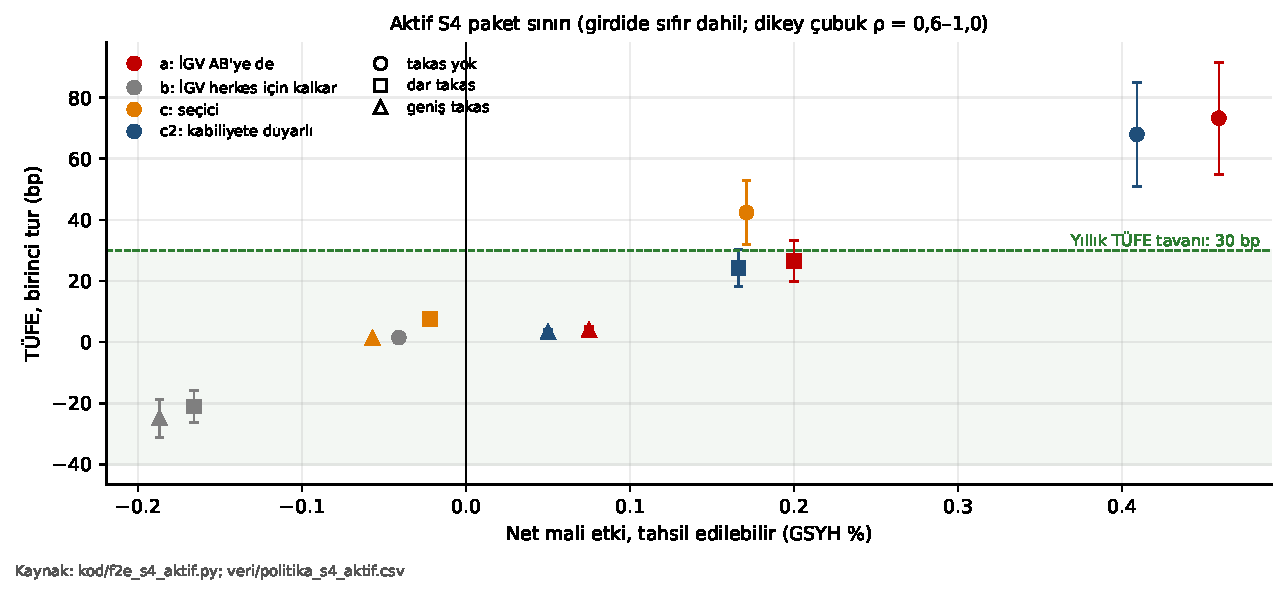
\includegraphics[width=1\textwidth,height=\textheight]{sekiller/f2_s4_paket_siniri.pdf}

\emph{Şekil 2A.2 --- Aktif S4 paket sınırı: birinci tur TÜFE ve tahsil edilebilir net mali etki (girdide sıfır dahil)}

\textbf{Okuma.}

\begin{enumerate}
\def\labelenumi{\arabic{enumi}.}
\item
  \textbf{Enflasyon kısıtı aktif tasarımla karşılanabiliyor.} İlk yıl 30 bp altında kalan dört paket:

  \begin{itemize}
  \tightlist
  \item
    c + dar: 7,5 bp;
  \item
    c2 + geniş: 3,3 bp;
  \item
    a + geniş: 4,0 bp;
  \item
    b + yok: 1,5 bp.
  \end{itemize}

  c2 + dar (24 bp) ve a + dar (27 bp) yıllık tavanın altında kalıyor, ama kümülatif 50 bp bütçesinin yarısını tüketiyor.
\item
  \textbf{Paketler arasında gerçek bir seçim var.} Bedel üç yerden ödeniyor: bütçe, koruma ve AB'ye verilen sinyal.

  \begin{itemize}
  \tightlist
  \item
    \textbf{b} en ucuz enflasyon çözümü. Ama Çin ve diğer kaynaklara karşı \$2,9 mlr'lık İGV korumasını yurt içi üretimi güçlü satırlarda kaldırır. Bu, Faz 3'teki kabiliyet kısıtıyla çatışır.
  \item
    \textbf{c} (Faz 2 ara raporundaki öneri) korumanın \$0,7 mlr'ını kaldırır ve mobilya ile kozmetikte yerli üreticiye zarar verir (§1.5). Mali olarak hafif negatif.
  \item
    \textbf{c2 + geniş} korumayı tamamen korur, TÜFE'yi 3,3 bp'de tutar ve tahsil edilebilir gelirle bile hafif pozitif kalır. Ayrıca S4'ün net istihdam kaybını −117 binden ≈ −35 bine indirir (§4.2). Bedeli daha geniş bir vergi takası (\$5,7 mlr ÖTV/KDV indirimi) ve daha karmaşık bir uygulama.
  \item
    \textbf{a + geniş}: c2'den farkı, İGV'nin kabiliyeti zayıf satırlarda da AB'ye uygulanması. Mali olarak biraz daha iyi, ama AB'den gelen ve yurt içinde üretilmeyen girdileri gereksiz yere pahalılaştırır.
  \end{itemize}
\item
  \textbf{Öneri: c2 + P1 + geniş takas.}

  \begin{itemize}
  \tightlist
  \item
    ``Geniş'' kapsamın pratik karşılığı şöyle: dar kapsama mobilya (KDV), gıda ve içecek (KDV) ve plastik ürünler eklenir.
  \item
    Bu üç ürün, c2'de dar takastan sonra kalan TÜFE etkisinin ≈\%80'ini oluşturuyor: mobilya 11,5 bp, gıda 5,9 bp, plastik 1,9 bp.
  \item
    Bu paket aynı zamanda AB'nin anlaşmasızlık maliyetini \$28,5 mlr'a çıkarıyor; c'de \$18,7 mlr. Müzakere kaldıracı açısından da en güçlüsü.
  \end{itemize}
\item
  \textbf{Takas bütçeyi değil, vergi yapısını değiştirir.}

  \begin{itemize}
  \tightlist
  \item
    Geniş takas, ÖTV ve KDV'de yılda ≈\$5,7 mlr indirim demek: 2025 ÖTV + KDV tahsilatının ≈\%3'ü.
  \item
    Bu indirim, AB mallarından alınan gümrük geliriyle finanse edilir.
  \item
    Net etki küçüktür. Ama vergi bileşimi tüketimden dış ticarete kayar. Bu tercihin orta vadede gözden geçirilmesi gerekir (Faz 6).
  \end{itemize}
\end{enumerate}

\hypertarget{02a_politika_uzayi-42-net-istihdam-ihracat-kaybux131-ve-ithal-ikamesi}{%
\subsection{4.2 Net istihdam: ihracat kaybı ve ithal ikamesi}\label{02a_politika_uzayi-42-net-istihdam-ihracat-kaybux131-ve-ithal-ikamesi}}

Faz 1'deki S4 risk istihdamı (207 bin) yalnızca ihracat tarafıydı. Türkiye de AB mallarına tarife uyguladığında AB'den ithalatın bir kısmı yurt içi üretime kayar. İthal ikamesinin büyüklüğü İGV rejimine bağlı. Aşağıda iki rejim var:

\begin{itemize}
\tightlist
\item
  AB'ye yalnızca MFN;
\item
  önerilen c2: İGV yurt içi üretimi güçlü satırlarda AB'ye de uygulanır.
\end{itemize}

\begingroup\gbtablo\small

\begin{longtable}[]{@{}lllr@{}}
\toprule\noalign{}
& \textbf{σ = 3} & \textbf{σ = 5} & \textbf{σ = 8} \\
\midrule\noalign{}
\endhead
\bottomrule\noalign{}
\endlastfoot
İhracat kaybı (\$ mlr) & −15,2 & −23,5 & −33,7 \\
İstihdam: ihracat tarafı & −123 bin & −190 bin & −272 bin \\
\emph{\textbf{AB'ye yalnızca MFN}} & & & \\
İthal ikamesiyle yurt içi satış artışı (\$ mlr) & +8,0 & +12,4 & +18,0 \\
İstihdam: ithal ikamesi & +47 bin & +73 bin & +106 bin \\
\textbf{Net imalat istihdamı} & \textbf{−77 bin} & \textbf{−117 bin} & \textbf{−165 bin} \\
Net kaybı \%5'i aşan / net kazanan sınıf & 14 / 61 & 22 / 61 & 32 / 61 \\
\emph{\textbf{Rejim c2 (önerilen)}} & & & \\
İthal ikamesiyle yurt içi satış artışı (\$ mlr) & +12,9 & +19,1 & +26,2 \\
İstihdam: ithal ikamesi & +100 bin & +142 bin & +187 bin \\
\textbf{Net imalat istihdamı} & \textbf{−24 bin} & \textbf{−48 bin} & \textbf{−84 bin} \\
Net kaybı \%5'i aşan / net kazanan sınıf & 11 / 99 & 21 / 95 & 28 / 88 \\
Vergi takasının on gruptaki ek etkisi (merkez; §1.5) & +12 bin & +12 bin & +12 bin \\
\textbf{Net, c2 + takas} & \textbf{≈ −11 bin} & \textbf{≈ −35 bin} & \textbf{≈ −72 bin} \\
\end{longtable}

\endgroup

\emph{Kaynak ve etiketler:}

\begin{itemize}
\tightlist
\item
  \etiketT{} \kod{kod/\allowbreak{}f2d\_\allowbreak{}s4\_\allowbreak{}net\_\allowbreak{}istihdam.\allowbreak{}py}, NACE sınıfı düzeyinde.
\item
  İhracat kaybı: Faz 0 S4 tarife duvarı (CN8).
\item
  İthal ikamesi: AB'den ithalatın kaybı. MFN satırında 2026 MFN (İGV hariç); c2 satırında HS6 düzeyinde rejim oranının AB ithalatı ağırlıklı ortalaması. Kaybı yerli ürünün iç pazardaki Armington payıyla yurt içine dağıttım. İç satış = max(PRODTR 2025, YSHİ 2024) − ihracat (BACI 2024).
\item
  İstihdam: YSHİ 2024 sınıf düzeyi çalışan/üretim oranı.
\item
  Takasın ek etkisi f2c'den alındı (T-A − pasif, rejim c2); σ ızgarası f2c'de farklı, bu yüzden merkez değer kullanıldı.
\item
  Statik ve telafisiz bir hesap. Çapa yatırımcı kararları, kapasite sınırları ve girdi bağlantıları yok. Yerli kapasitenin ithal ikamesini karşılayabileceği varsayıldı; büyük İGV şoklarında bu bir üst sınırdır.
\item
  Güven: Orta (c2 satırları için Düşük--Orta).
\end{itemize}

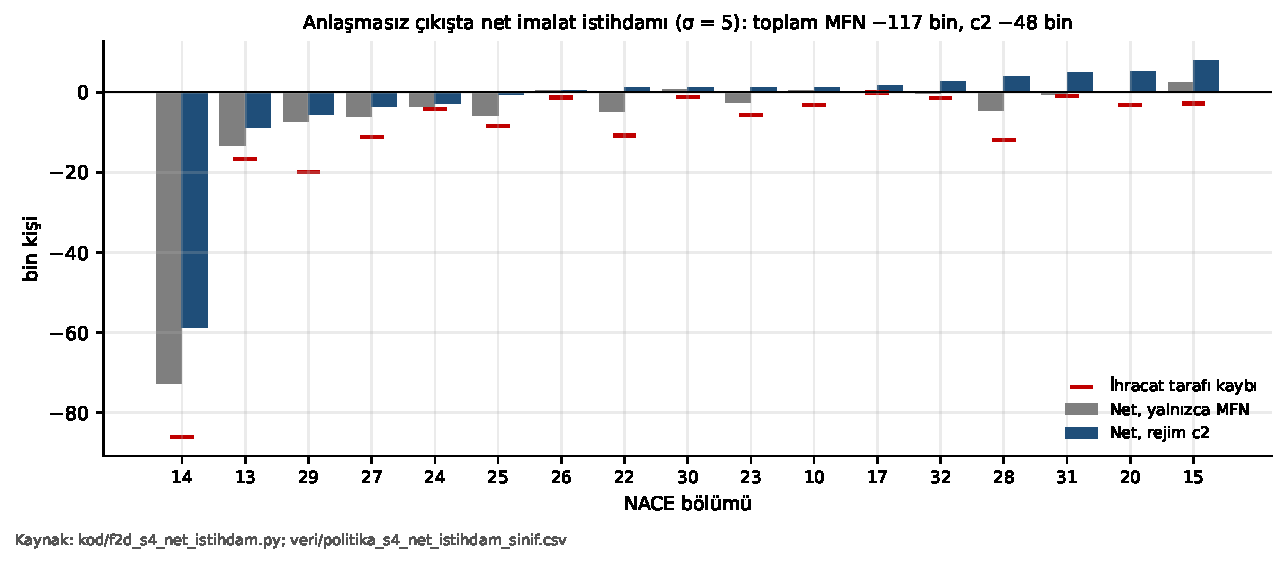
\includegraphics[width=1\textwidth,height=\textheight]{sekiller/f2_net_istihdam.pdf}

\emph{Şekil 2A.3 --- Anlaşmasız çıkışta NACE bölümü düzeyinde net imalat istihdamı: yalnızca MFN ve rejim c2 (σ = 5)}

\textbf{Bölüm düzeyinde net etki (σ = 5)}

\begingroup\gbtablo\footnotesize

\begin{longtable}[]{@{}
  >{\raggedright\arraybackslash}p{(\columnwidth - 16\tabcolsep) * \real{0.0703}}
  >{\raggedright\arraybackslash}p{(\columnwidth - 16\tabcolsep) * \real{0.1411}}
  >{\raggedleft\arraybackslash}p{(\columnwidth - 16\tabcolsep) * \real{0.0991}}
  >{\raggedleft\arraybackslash}p{(\columnwidth - 16\tabcolsep) * \real{0.1235}}
  >{\raggedleft\arraybackslash}p{(\columnwidth - 16\tabcolsep) * \real{0.1367}}
  >{\raggedleft\arraybackslash}p{(\columnwidth - 16\tabcolsep) * \real{0.1011}}
  >{\raggedleft\arraybackslash}p{(\columnwidth - 16\tabcolsep) * \real{0.1283}}
  >{\raggedleft\arraybackslash}p{(\columnwidth - 16\tabcolsep) * \real{0.0927}}
  >{\raggedleft\arraybackslash}p{(\columnwidth - 16\tabcolsep) * \real{0.1071}}@{}}
\toprule\noalign{}
\begin{minipage}[b]{\linewidth}\raggedright
\textbf{NACE}
\end{minipage} & \begin{minipage}[b]{\linewidth}\raggedright
\textbf{Bölüm}
\end{minipage} & \begin{minipage}[b]{\linewidth}\raggedleft
\textbf{Çalışan (bin)}
\end{minipage} & \begin{minipage}[b]{\linewidth}\raggedleft
\textbf{İhracat tarafı (bin)}
\end{minipage} & \begin{minipage}[b]{\linewidth}\raggedleft
\textbf{İthal ikamesi, MFN (bin)}
\end{minipage} & \begin{minipage}[b]{\linewidth}\raggedleft
\textbf{Net, MFN (bin)}
\end{minipage} & \begin{minipage}[b]{\linewidth}\raggedleft
\textbf{İthal ikamesi, c2 (bin)}
\end{minipage} & \begin{minipage}[b]{\linewidth}\raggedleft
\textbf{\textbf{Net, c2 (bin)}}
\end{minipage} & \begin{minipage}[b]{\linewidth}\raggedleft
\textbf{Net, c2 (\% bölüm)}
\end{minipage} \\
\midrule\noalign{}
\endhead
\bottomrule\noalign{}
\endlastfoot
14 & Giyim & 668,7 & −86,2 & +13,6 & −72,6 & +27,5 & \textbf{−58,7} & \textbf{−8,8} \\
13 & Tekstil & 493,4 & −16,7 & +3,4 & −13,3 & +7,8 & −8,9 & −1,8 \\
29 & Motorlu taşıtlar & 255,3 & −19,9 & +12,5 & −7,4 & +14,2 & −5,6 & −2,2 \\
27 & Elektrikli teçhizat & 231,6 & −11,2 & +5,1 & −6,1 & +7,7 & −3,5 & −1,5 \\
24 & Ana metal & 194,1 & −4,2 & +0,8 & −3,5 & +1,3 & −2,9 & −1,5 \\
25 & Fabrikasyon metal & 474,7 & −8,5 & +2,7 & −5,8 & +7,9 & −0,6 & −0,1 \\
22 & Kauçuk ve plastik & 283,5 & −10,8 & +5,9 & −4,9 & +11,9 & +1,1 & +0,4 \\
28 & Makine & 319,0 & −11,8 & +7,3 & −4,6 & +15,7 & +3,9 & +1,2 \\
30 & Diğer ulaşım araçları & 86,9 & −1,2 & +2,0 & +0,8 & +2,4 & +1,2 & +1,4 \\
10 & Gıda & 610,3 & −3,1 & +3,7 & +0,6 & +4,4 & +1,3 & +0,2 \\
31 & Mobilya & 252,8 & −1,0 & +0,3 & −0,6 & +6,0 & +5,0 & +2,0 \\
20 & Kimya & 128,0 & −3,3 & +3,6 & +0,3 & +8,4 & +5,1 & +4,0 \\
15 & Deri ve ayakkabı & 75,8 & −2,8 & +5,2 & +2,4 & +10,7 & \textbf{+7,9} & +10,5 \\
\end{longtable}

\endgroup

\emph{Kaynak:} \etiketT{} \kod{veri/\allowbreak{}politika\_\allowbreak{}s4\_\allowbreak{}net\_\allowbreak{}istihdam\_\allowbreak{}sinif.\allowbreak{}csv}.

\textbf{Net kaybı \%5'i aşan sınıflar (σ = 5).}

\begin{itemize}
\tightlist
\item
  MFN'de 22 sınıf:

  \begin{itemize}
  \tightlist
  \item
    10.86; 13.92;
  \item
    giyim: 14.13, 14.14, 14.19, 14.31, 14.39;
  \item
    20.14, 23.42, 24.42, 25.99;
  \item
    26.52, 26.70, 27.11, 27.90;
  \item
    28.11, 28.15, 28.24;
  \item
    29.10, 30.92, 32.13, 32.20.
  \end{itemize}
\item
  c2'de 21 sınıf: 23.42 ve 25.99 listeden çıkıyor, 26.30 giriyor.
\end{itemize}

Bu sınıflar ana promptun destek tetikleyicisini (\textgreater\%5 kayıp) çalıştırır ve Faz 3'te ayrı ayrı ele alınacak.

\textbf{Okuma.}

\begin{itemize}
\tightlist
\item
  \textbf{İGV rejimi istihdam için de belirleyici.}

  \begin{itemize}
  \tightlist
  \item
    Yalnızca MFN'de ithal ikamesi ihracat kaybının \%38'ini geri kazandırıyor; c2'de \%75'ini.
  \item
    Nedeni: İGV yurt içi üretimi güçlü satırlarda AB'ye de uygulanınca AB ithalatının yerini büyük ölçüde yerli üretim alıyor. Bu satırlar giyim, ayakkabı, mobilya, kimya ve plastik.
  \end{itemize}
\item
  \textbf{Kaybın yapısı ise değişmiyor.}

  \begin{itemize}
  \tightlist
  \item
    Otomotivde (29.10) iç pazar AB ithalatının yerini alabiliyor: ihracat tarafı −14,8 bin, ikame +9,9 bin. Takasla birlikte ikame +10,6 bine çıkıyor.
  \item
    Giyim (14) bunu yapamıyor. İç pazarda AB'nin payı küçük (≈\%2--5); kayıp AB pazarında.
  \end{itemize}
\item
  \textbf{Giyim, S4'te istihdam kısıtının çözülemeyen çekirdeği:} c2 ve takasla bile ≈ −50 bin.

  \begin{itemize}
  \tightlist
  \item
    AB'nin \%12'lik MFN'sine karşı rakipler sıfır tarifeyle giriyor: Bangladeş (``Silah Hariç Her Şey'' rejimi, EBA) ile AB'nin STA ortakları Fas, Tunus ve Vietnam.
  \item
    Türkiye'nin AB giyim ithalatındaki payı zaten düşüşte (Faz 1).
  \item
    Bu sınıflar S4'te F arketipine (yönetilen uyum) girer. S2/S3'te ise menşe kuralı belirleyici olur (giyimde çift dönüşüm).
  \end{itemize}
\end{itemize}

\hypertarget{02a_politika_uzayi-43-cari-denge-ve-reel-kur}{%
\subsection{4.3 Cari denge ve reel kur}\label{02a_politika_uzayi-43-cari-denge-ve-reel-kur}}

\begin{itemize}
\tightlist
\item
  \textbf{İlk yıl, kısmi denge.}

  \begin{itemize}
  \tightlist
  \item
    AB'ye ihracat kaybı −€21,5 mlr (σ = 5).
  \item
    AB'den ithalat kaybı −€19,9 mlr (yalnızca MFN; Faz 0, Comext tabanı) ile ≈−\$28,5 mlr (c2; BACI tabanı) arasında. Bunun ≈\%40'ı yurt içi üretime, kalanı diğer kaynaklara kayar.
  \item
    Doğrudan cari denge etkisi ≈ −\$12 ile −\$16 mlr: 2028 GSYH'sinin −0,6 ile −0,8 puanı. \etiketT{} Güven: Düşük.
  \end{itemize}
\item
  \textbf{Genel denge.} Lerner simetrisi ve reel kur tepkisi devreye girer:

  \begin{itemize}
  \tightlist
  \item
    TL'nin reel değer kaybı ihracat kaybını kısmen telafi eder, ama dezenflasyonu zorlar.
  \item
    Tasarruf-yatırım dengesi değişmedikçe kalıcı cari denge etkisi sıfıra yakın olur (Furceri vd. 2019; temel ilke 5).
  \item
    S4 cari denge hedefine katkı vermez. Hedef, Faz 1 §3.6'daki tamamlayıcı politikalara bağlı.
  \end{itemize}
\end{itemize}

\hypertarget{02a_politika_uzayi-44-abnin-maliyeti-ve-pazarlux131k-guxfccuxfc}{%
\subsection{4.4 AB'nin maliyeti ve pazarlık gücü}\label{02a_politika_uzayi-44-abnin-maliyeti-ve-pazarlux131k-guxfccuxfc}}

\begingroup\gbtablo\small

\begin{longtable}[]{@{}
  >{\raggedright\arraybackslash}p{(\columnwidth - 4\tabcolsep) * \real{0.1753}}
  >{\raggedright\arraybackslash}p{(\columnwidth - 4\tabcolsep) * \real{0.6830}}
  >{\raggedright\arraybackslash}p{(\columnwidth - 4\tabcolsep) * \real{0.1416}}@{}}
\toprule\noalign{}
\begin{minipage}[b]{\linewidth}\raggedright
\end{minipage} & \begin{minipage}[b]{\linewidth}\raggedright
\textbf{Değer}
\end{minipage} & \begin{minipage}[b]{\linewidth}\raggedright
\textbf{Kaynak}
\end{minipage} \\
\midrule\noalign{}
\endhead
\bottomrule\noalign{}
\endlastfoot
AB--Türkiye mal ticareti, 2025 & €217,6 mlr; AB ihracatı €114,3 mlr, ithalatı €103,3 mlr (AB fazlası ≈€11 mlr) & \etiketV{} Komisyon \\
Türkiye'nin AB için sırası & 5. ticaret ortağı; hizmet ticareti €42,1 mlr (2024) & \etiketV{} \\
Otomotiv & Türkiye, AB yeni araç ihracatının 3. büyük pazarı: 811.957 araç, €18,8 mlr, değerin \%11,1'i. Türkiye'nin AB'ye arzı 797.721 araç, €18,2 mlr; AB yeni araç ithalatının \%21,5'i (230.833'ü ticari araç ve otobüs, €8,2 mlr). Türk pazarında AB üretimi araçların payı \%49, Çin'in \%8 & \etiketV{} ACEA, Temmuz 2026 \\
AB'nin anlaşmasızlık kaybı (σ = 5) & Yalnızca MFN (b) \$16,4 mlr; c \$18,7 mlr; c2 \$28,5 mlr; a \$31,1 mlr. Karşılaştırma: Türkiye'nin AB'ye ihracat kaybı €21,5 mlr & \etiketT{} §4.1 \\
Göreli yük & AB'de GSYH'nin ≈\%0,1--0,2'si; Türkiye'de ≈\%1,5'i & \etiketT{} \\
\end{longtable}

\endgroup

\textbf{Okuma.}

\begin{itemize}
\tightlist
\item
  Kayıplar değer olarak benzer, ekonomilerin büyüklüğüne göre değil. Asimetri Türkiye aleyhine.
\item
  Ama AB'nin kaybı otomotivde ve birkaç üye devlette yoğunlaşıyor. Almanya, İspanya, Fransa, Çekya, Slovakya ve Romanya Türkiye'ye en çok otomobil satan ülkeler.
\item
  Renault, Stellantis, Ford, Toyota, Hyundai ve Mercedes'in Türkiye'deki fabrikaları AB pazarına üretiyor. AB tedarik zincirleri iki yönlü.
\item
  AB'nin md. 207 kapsamındaki kararları nitelikli çoğunlukla alınıyor. Almanya ve İtalya'nın pozisyonu belirleyici; Yunanistan ve GKRY'nin nüfus payı ≈\%2,5 (§6).
\item
  Aktif S4, Türkiye'nin anlaşmasızlık maliyetini enflasyon tarafında düşürür. AB'nin otomotiv maliyetini ise artırır. \textbf{Bu, Türkiye'nin anlaşmasız alternatifini (BATNA) güçlendirir} ve Faz 7'deki müzakere stratejisinin temel kozlarından biridir.
\item
  \etiketT{}/\etiketH{} Güven: Orta.
\end{itemize}

\textbf{AB'nin karşı araçları.} Hasmane AB varsayımında bunlar zaten kullanılıyor veya kullanılabilir:

\begingroup\gbtablo\small

\begin{longtable}[]{@{}
  >{\raggedright\arraybackslash}p{(\columnwidth - 4\tabcolsep) * \real{0.1786}}
  >{\raggedright\arraybackslash}p{(\columnwidth - 4\tabcolsep) * \real{0.4154}}
  >{\raggedright\arraybackslash}p{(\columnwidth - 4\tabcolsep) * \real{0.4060}}@{}}
\toprule\noalign{}
\begin{minipage}[b]{\linewidth}\raggedright
\textbf{Araç}
\end{minipage} & \begin{minipage}[b]{\linewidth}\raggedright
\textbf{Tetikleyici}
\end{minipage} & \begin{minipage}[b]{\linewidth}\raggedright
\textbf{Türkiye için anlamı}
\end{minipage} \\
\midrule\noalign{}
\endhead
\bottomrule\noalign{}
\endlastfoot
Uygulama Tüzüğü 654/2014 (2021/167 ile değişik) & DTÖ kararı, temyizi engellenmiş panel raporu (md. 3(aa)), ikili anlaşmada işbirliği reddi (md. 3(ba)), XXVIII dengelemesi (md. 3(d)) & Tek taraflı GB değişikliğine karşı ana araç \\
Zorlamaya Karşı Araç (2023/2675) & AB veya üye devletin egemen tercihine yönelik ekonomik baskı & Yalnızca ticari baskı GKRY veya Yunanistan meselesine bağlanırsa \\
Çelik tüzüğü 2026/1384 (17.6.2026) & Küresel kapasite fazlası; md. 207(2); DTÖ korunma anlaşması dışında & 18,35 Mt kota; kota dışı \%50 vergi; 1.10.2026'dan itibaren ``eritildiği ve döküldüğü yer'' kuralı. Türkiye'nin payı en büyük: ≈2,86 Mt. Çelik GB dışında olduğu için çıkıştan bağımsız olarak geçerli \\
Ticaret savunması & 2024--26'da Türkiye'ye karşı: sıcak haddelenmiş yassı çelik, seramik karo, balık (alabalık), dolanma önleme kararları; soğuk haddelenmiş çelik, kaynaklı çelik hasır ve tel halat soruşturmaları & Çıkıştan sonra artabilir \\
Onaylanmış kuruluşlar, SKDM, menşe kuralları & ACAA/MRA yokluğunda Türk sertifikalarının AB geçerliliği biter; SKDM karbon maliyeti & İhracatçının uyum maliyeti \\
Siyasi araçlar & SAFE savunma fonu (oybirliği; Yunanistan ve GKRY şartı), vize, göç ve enerji dosyaları & Hasmane AB varsayımında (V-11) zaten kullanılıyor \\
\end{longtable}

\endgroup

\emph{Kaynak:} \etiketV{} AB hukuku araştırma notu S12, S18, S20--S23; \etiketD{} basında geçen Türk lastiğine anti-damping iddiası Resmî Gazete'de bulunamadı.

\hypertarget{02a_politika_uzayi-45-sonuuxe7-aktif-tasarux131m-faz-1-teux15fhisini-nasux131l-deux11fiux15ftiriyor}{%
\subsection{4.5 Sonuç: aktif tasarım Faz 1 teşhisini nasıl değiştiriyor?}\label{02a_politika_uzayi-45-sonuuxe7-aktif-tasarux131m-faz-1-teux15fhisini-nasux131l-deux11fiux15ftiriyor}}

\begingroup\gbtablo\small

\begin{longtable}[]{@{}
  >{\raggedright\arraybackslash}p{(\columnwidth - 6\tabcolsep) * \real{0.1825}}
  >{\raggedright\arraybackslash}p{(\columnwidth - 6\tabcolsep) * \real{0.2533}}
  >{\raggedright\arraybackslash}p{(\columnwidth - 6\tabcolsep) * \real{0.3004}}
  >{\raggedright\arraybackslash}p{(\columnwidth - 6\tabcolsep) * \real{0.2639}}@{}}
\toprule\noalign{}
\begin{minipage}[b]{\linewidth}\raggedright
\textbf{Kısıt}
\end{minipage} & \begin{minipage}[b]{\linewidth}\raggedright
\textbf{Pasif S4 (Faz 1)}
\end{minipage} & \begin{minipage}[b]{\linewidth}\raggedright
\textbf{Aktif S4 (c2 + P1 + geniş takas)}
\end{minipage} & \begin{minipage}[b]{\linewidth}\raggedright
\textbf{Değerlendirme}
\end{minipage} \\
\midrule\noalign{}
\endhead
\bottomrule\noalign{}
\endlastfoot
Enflasyon (≤30 bp/yıl, ≤50 bp kümülatif) & 59--98 bp: ihlal & 2,5--4,1 bp: \textbf{sağlanıyor} & Takas ve İGV tasarımı yeterli \\
Mali (≤ GSYH \%0,5/yıl) & Gelir artışı & +\%0,05 (tahsil edilebilir) & Sağlanıyor \\
İstihdam (T+3'te net sıfır) & −207 bin (brüt); −117 bin (net, yalnızca MFN) & ≈ −35 bin (net, σ = 5; ≈ −11 ile −72 bin) & \textbf{İhlal}, ama dar: giyim −58,7 bin, diğer bölümler toplamda ≈ +11 bin \\
Kabiliyet & Otomotiv, giyim ve beyaz eşya ihracat platformlarında risk & İç pazarda koruma korunuyor; ihracat platformu riski değişmiyor & \textbf{İhlal riski} \\
Cari denge & İlk yıllarda −0,6 ile −0,8 puan & Değişmiyor & Tamamlayıcı politikalar şart \\
DTÖ uyumu & --- & Uyumlu: MFN, bağlı oran içinde, menşeden bağımsız vergi; XXVIII:5 çekincesiyle esneklik & Sağlanıyor \\
\end{longtable}

\endgroup

\emph{Not:} Aktif S4'ün istihdam sütunu f2d'nin c2 hesabıdır; takasın on gruptaki ek etkisi (+12 bin) eklendi \etiketT{}. Kapasite sınırları ve çapa yatırımcı kararları dahil değil (§4.2).

\textbf{Teşhisin yeni hali.}

\begin{itemize}
\tightlist
\item
  S4'ün enflasyon sorunu, Türkiye'nin kendi araçlarıyla çözülebilen bir tasarım sorunudur.
\item
  S4'ün istihdam, kabiliyet ve ihracat sorunları ise Türkiye'nin kontrolü dışında. Belirleyici olan AB'nin tarifeleri ve menşe kurallarıdır.
\item
  Bu yüzden S4 hâlâ bitiş durumu olamaz. Ama geri dönüş planı olarak çok daha az maliyetli ve müzakerede caydırıcı bir alternatif.
\end{itemize}

\begin{center}\rule{0.5\linewidth}{0.5pt}\end{center}

\hypertarget{02a_politika_uzayi-5-iux307hracat-tarafux131-tuxfcrkiyenin-elinde-ne-var-ne-yok}{%
\section{5. İhracat tarafı: Türkiye'nin elinde ne var, ne yok?}\label{02a_politika_uzayi-5-iux307hracat-tarafux131-tuxfcrkiyenin-elinde-ne-var-ne-yok}}

\begingroup\gbtablo\small

\begin{longtable}[]{@{}
  >{\raggedright\arraybackslash}p{(\columnwidth - 6\tabcolsep) * \real{0.1771}}
  >{\raggedright\arraybackslash}p{(\columnwidth - 6\tabcolsep) * \real{0.2744}}
  >{\raggedright\arraybackslash}p{(\columnwidth - 6\tabcolsep) * \real{0.3602}}
  >{\raggedright\arraybackslash}p{(\columnwidth - 6\tabcolsep) * \real{0.1882}}@{}}
\toprule\noalign{}
\begin{minipage}[b]{\linewidth}\raggedright
\textbf{Seçenek}
\end{minipage} & \begin{minipage}[b]{\linewidth}\raggedright
\textbf{Hukuki durum}
\end{minipage} & \begin{minipage}[b]{\linewidth}\raggedright
\textbf{Ekonomik etkinlik}
\end{minipage} & \begin{minipage}[b]{\linewidth}\raggedright
\textbf{Değerlendirme}
\end{minipage} \\
\midrule\noalign{}
\endhead
\bottomrule\noalign{}
\endlastfoot
İhracat sübvansiyonu (AB tarifesini telafi) & \textbf{Yasak} (ASCM 3.1(a)) & --- & Kullanılamaz \\
Üretim sübvansiyonu (ihracata bağlı değil) & Dava edilebilir (ASCM 5--6); AB'de telafi edici vergiye açık & AB'nin S4'te alacağı ≈\$6,1 mlr vergiyi telafi etmek için bütün üretime ödeme gerekir: yılda ≈\$38 mlr (2028 GSYH'sinin \%1,8'i). Otomotivde \$2,2 mlr vergi için \$5,6 mlr. AB bu desteği telafi edici vergiyle geri alır & Mali tavanın çok üstünde ve etkisiz. \textbf{Kullanılmamalı} \\
Kur & DTÖ'de sorun yok (2026'da ABD'nin telafi edici vergi soruşturmalarında ``kur düşüklüğü'' iddiası gündemde) & Dezenflasyonla çatışır & Kullanılmamalı \\
Pazar çeşitlendirmesi (STA ağı) & Uyumlu & Orta vadede. AB pazarının yerini 5 yılda alamaz: Türkiye'nin asimetrik pazarlara ihracatı \$17,6 mlr, AB'ye \$119,5 mlr & Gerekli ama yetersiz \\
Menşe ve uyum kolaylığı (S2/S3) & Anlaşmaya bağlı & En etkili: sıfır tarifeyi korur & \textbf{Ana yol} \\
Çapa yatırımcıyla tutma sözleşmesi & Uyumlu; performans koşulları ihracata bağlı sübvansiyon içermemeli & Kararı AB pazarına erişim belirler & Tamamlayıcı \\
Geçiş dönemi ve dondurma & Anlaşmaya bağlı (XXIV:5; Ortaklık Konseyi kararı) & Uçurumu önler & T2028 için şart \\
Eximbank kredileri ve DİR & OECD Uzlaşması içindeyse ve DİR normlara bağlıysa düşük risk & Finansman maliyetini düşürür, tarife farkını kapatmaz & Tamamlayıcı \\
\end{longtable}

\endgroup

\emph{Kaynak:} \etiketT{} tam telafi maliyeti = AB'nin ağırlıklı MFN'si × bölüm üretim değeri (YSHİ 2024), \kod{veri/\allowbreak{}teshis\_\allowbreak{}bolum\_\allowbreak{}maruziyet.\allowbreak{}csv}. Güven: Orta.

\textbf{Sonuç.} İhracat tarafında AB'nin tarifesi iç politikayla telafi edilemez. Telafi girişimi ya yasaktır, ya mali tavanı aşar, ya da AB'nin telafi edici vergisiyle boşa çıkar. Bu yüzden çıkışın ihracat cephesi bir anlaşmaya bağlıdır: S2, S3 veya en azından geçiş anlaşması.

\begin{center}\rule{0.5\linewidth}{0.5pt}\end{center}

\hypertarget{02a_politika_uzayi-6-dux131ux15f-rejim-seuxe7enekleri-evreni}{%
\section{6. Dış rejim seçenekleri evreni}\label{02a_politika_uzayi-6-dux131ux15f-rejim-seuxe7enekleri-evreni}}

S0--S5 ana promptun senaryolarıdır. Aşağıda bunların yanında melez ve geçiş modelleri de var. Hukuki mekanik, şablonlar, menşe ve uyum değerlendirmesi, takvim ve sayısal karşılaştırma \belgebag{02b_secenekler_hukuk}{}{\kod{02b\_\allowbreak{}secenekler\_\allowbreak{}hukuk.\allowbreak{}md}}'de.

\begingroup\gbtablo\footnotesize

\begin{longtable}[]{@{}
  >{\raggedright\arraybackslash}p{(\columnwidth - 12\tabcolsep) * \real{0.0439}}
  >{\raggedright\arraybackslash}p{(\columnwidth - 12\tabcolsep) * \real{0.1157}}
  >{\raggedright\arraybackslash}p{(\columnwidth - 12\tabcolsep) * \real{0.1770}}
  >{\raggedright\arraybackslash}p{(\columnwidth - 12\tabcolsep) * \real{0.1902}}
  >{\raggedright\arraybackslash}p{(\columnwidth - 12\tabcolsep) * \real{0.2037}}
  >{\raggedright\arraybackslash}p{(\columnwidth - 12\tabcolsep) * \real{0.1144}}
  >{\raggedright\arraybackslash}p{(\columnwidth - 12\tabcolsep) * \real{0.1551}}@{}}
\toprule\noalign{}
\begin{minipage}[b]{\linewidth}\raggedright
\textbf{No}
\end{minipage} & \begin{minipage}[b]{\linewidth}\raggedright
\textbf{Model}
\end{minipage} & \begin{minipage}[b]{\linewidth}\raggedright
\textbf{İçerik}
\end{minipage} & \begin{minipage}[b]{\linewidth}\raggedright
\textbf{DTÖ dayanağı}
\end{minipage} & \begin{minipage}[b]{\linewidth}\raggedright
\textbf{AB tarafında hukuki yol ve oy kuralı}
\end{minipage} & \begin{minipage}[b]{\linewidth}\raggedright
\textbf{Hasmane AB'de gerçekçilik \etiketH{}}
\end{minipage} & \begin{minipage}[b]{\linewidth}\raggedright
\textbf{Not}
\end{minipage} \\
\midrule\noalign{}
\endhead
\bottomrule\noalign{}
\endlastfoot
R1 & Statüko GB (S0) & Mevcut 1/95 & XXIV:8(a) & --- & --- & Referans \\
R2 & Modernize GB (S1) & Hizmetler, kamu alımı, tarım, uyuşmazlık çözümü & XXIV & Konsey müzakere yönergesi hiç kabul edilmedi (Komisyon önerisi Aralık 2016) & Düşük & Karşı-olgu \\
R3 & Derin ve kapsamlı STA, DCFTA (S2) & Sanayide sıfır tarife, PEM menşei ve tam kümülasyon, ACAA, hizmetler, kamu alımı, karayolu ve vize & XXIV:8(b) & Md. 207 (nitelikli çoğunluk; hizmet ve fikrî mülkiyette md. 207(4) gereği oybirliği olabilir) veya md. 217 (oybirliği) & Orta--düşük & 2030 sonrası \\
R4 & Temel STA (S3) & Sıfır tarife, PEM menşei, ACAA yok & XXIV:8(b) & Md. 207 (nitelikli çoğunluk) + Avrupa Parlamentosu onayı & Orta & T2029 için en fazla bu \\
R5 & İsviçre modeli & 1972 tipi sanayi STA'sı + sektörel anlaşmalar (MRA, taşımacılık) & XXIV & Birden çok anlaşma; 2026 kurumsal paketi dinamik uyum ve AB Adalet Divanı rolü içeriyor & Düşük (zaman) & Parçalı ilerleme imkânı \\
R6 & Birleşik Krallık TCA modeli & Sıfır tarife ve kota; yalnızca ikili kümülasyon; eşit rekabet koşulları ve md. 411 yeniden dengeleme; 12 ay ihbarla fesih & XXIV & Md. 217 (oybirliği) & Orta & ≈10 aylık müzakere emsali; hazır yetki ve varoluşsal son tarih gerektirdi \\
R7 & \textbf{Geçici anlaşma ve dondurma} & GB tercihleri sabit bir tarihe kadar korunur (ör. 31.12.2029); STA'ya geçiş takvimi & XXIV:5(c); makul süre en fazla 10 yıl & Ortaklık Konseyi kararı (AB pozisyonu md. 207(4) + 218(9), nitelikli çoğunluk; C-81/13). Kurumsal çerçeveyi değiştiremez; GB'yi kaldıramaz, dondurabilir ve aşamalandırabilir & Orta (AB'nin otomotiv çıkarı var) & \textbf{T2028 için tek gerçekçi yol} \\
R8 & Geçici Ticaret Anlaşması (ITA) ayrımı & AB'nin tek başına yetkili olduğu bir md. 207 anlaşması GB hükümlerini ``etkisiz kılar''; karma ortaklık anlaşması sonra gelir & XXIV:5--8 & AB--Şili ITA md. 33.11 (``Ortaklık Anlaşmasının IV. Kısmı \ldots{} etkisiz kalır''); Mercosur: Konsey Kararı 2026/183, nitelikli çoğunlukla. AB Adalet Divanı'nın 1/26 sayılı görüşü bekleniyor: ayrım tekniğini daraltabilir & Orta--düşük & T2029'un hukuki aracı \\
R9 & Asimetrik geçiş & AB sıfır, Türkiye AB mallarına kademeli tarife indirimi (veya tersi) & XXIV (asimetri kabul edilir) & Md. 207 & Düşük & Hasmane AB kabul etmez \\
R10 & Sektörel GB (ör. yalnızca otomotiv) & --- & \textbf{XXIV'e aykırı}: ``ticaretin esasının tamamı'' şartı ``ticaretin yalnızca bir kısmından çok daha fazlası'' demek (Türkiye--Tekstil, DS34, para. 48) & --- & Yok & Kullanılamaz \\
R11 & GB'de kalıp STA özerkliği & Ortak dış tarifesiz GB & GB tanımına aykırı & --- & Yok & Kullanılamaz \\
R12 & EFTA üyeliği & EFTA Sözleşmesi md. 56 & --- & AB pazarına erişim sağlamaz (AEA dışı) & Düşük fayda & Türkiye--EFTA STA'sı zaten var \\
R13 & \textbf{Aktif S4} & Anlaşmasız çıkış + tek taraflı paket (§4: c2 + P1 + geniş takas) & DTÖ & --- & Yüksek olasılıklı geri dönüş planı & Enflasyon kısıtını çözer; ihracat ve istihdam kısıtlarını çözmez; BATNA'yı güçlendirir \\
R14 & S5 (gerilim) & S4 + AB ticaret savunmasında sertleşme, kritik girdi kısıtı, risk primi & DTÖ & Uygulama Tüzüğü, çelik tüzüğü, Zorlamaya Karşı Araç & Stres testi & \\
R15 & Tek taraflı fesih & Ankara Anlaşması ve 1/95'te fesih hükmü yok; teamül hukuku (Viyana Sözleşmesi md. 56 ve 62'nin karşılığı) feshi ancak niyet veya köklü değişiklik varsa kabul eder. Türkiye Viyana Sözleşmesi'ne taraf değil & --- & AB, md. 58(2) koruma önlemleri, md. 64 yeniden dengeleme ve Uygulama Tüzüğü md. 3(ba) ile karşılık verebilir & Yüksek riskli & Hukuken açık; yalnızca son çare \\
R16 & Kademeli çıkış & Önce STA ağı ve tarife cetveli hazırlanır; GB'den çıkış anlaşmayla eş zamanlı & --- & --- & Yüksek (iç hazırlık) & Temel ilke 1 ve 10 \\
R17 & Çok taraflı açılım & ABD ile sektörel tarife anlaşması; Hindistan, Mercosur, Japonya STA'ları; KİK & XXIV & --- & Orta & Çıkışla aynı anda başlar \\
\end{longtable}

\endgroup

\emph{Kaynak ve etiketler:}

\begin{itemize}
\tightlist
\item
  \etiketV{} Ankara Anlaşması (md. 23, 25, 31--33); 1/95 sayılı Karar (md. 13, 58, 61--64); ABİDA md. 207, 217, 218.
\item
  C-81/13 İngiltere/Konsey; AB--Şili ITA (L\_202402953); Konsey Kararı 2026/183; COM(2026) 477; DS34 Temyiz Organı raporu.
\item
  \etiketH{} gerçekçilik yargısı. Güven: Orta.
\end{itemize}

\textbf{Kısa liste.} Faz 2B'de karşılaştırılacaklar:

\begin{itemize}
\tightlist
\item
  S0, S1, S2, S3;
\item
  R7 (dondurma ve geçici anlaşma), R8 (ITA ayrımı);
\item
  aktif S4 (R13) ve S5;
\item
  bunların T2028 ve T2029 takvimlerine göre sıralanmış bileşimleri (ör. ``R7 → S3 → S2'').
\end{itemize}

\begin{center}\rule{0.5\linewidth}{0.5pt}\end{center}

\hypertarget{02a_politika_uzayi-7-zaman-kritik-eylemler-pazartesi-sabahux131-listesi-faz-2a}{%
\section{7. Zaman kritik eylemler (``Pazartesi sabahı'' listesi, Faz 2A)}\label{02a_politika_uzayi-7-zaman-kritik-eylemler-pazartesi-sabahux131-listesi-faz-2a}}

\begingroup\gbtablo\footnotesize

\begin{longtable}[]{@{}
  >{\raggedright\arraybackslash}p{(\columnwidth - 10\tabcolsep) * \real{0.0204}}
  >{\raggedright\arraybackslash}p{(\columnwidth - 10\tabcolsep) * \real{0.2797}}
  >{\raggedright\arraybackslash}p{(\columnwidth - 10\tabcolsep) * \real{0.1510}}
  >{\raggedright\arraybackslash}p{(\columnwidth - 10\tabcolsep) * \real{0.1821}}
  >{\raggedright\arraybackslash}p{(\columnwidth - 10\tabcolsep) * \real{0.1247}}
  >{\raggedright\arraybackslash}p{(\columnwidth - 10\tabcolsep) * \real{0.2420}}@{}}
\toprule\noalign{}
\begin{minipage}[b]{\linewidth}\raggedright
\textbf{\#}
\end{minipage} & \begin{minipage}[b]{\linewidth}\raggedright
\textbf{Eylem}
\end{minipage} & \begin{minipage}[b]{\linewidth}\raggedright
\textbf{Sorumlu}
\end{minipage} & \begin{minipage}[b]{\linewidth}\raggedright
\textbf{Hukuki araç}
\end{minipage} & \begin{minipage}[b]{\linewidth}\raggedright
\textbf{Son tarih}
\end{minipage} & \begin{minipage}[b]{\linewidth}\raggedright
\textbf{Neden şimdi}
\end{minipage} \\
\midrule\noalign{}
\endhead
\bottomrule\noalign{}
\endlastfoot
1 & \textbf{GATT XXVIII:5 çekincesi}: 1.1.2027'de başlayan dönem için Cetvel XXXVII'yi değiştirme hakkının saklı tutulması & Dışişleri Bakanlığı (Cenevre Daimi Temsilciliği) ve Ticaret Bakanlığı & DTÖ Mal Ticareti Konseyi'ne nota & \textbf{31.12.2026} & Çıkış 2028 veya 2029'da; bağlı oranlarda esneklik ancak bu dönem için şimdi saklı tutulabilir. Bedeli: diğer üyelerin de Türkiye ile ilk müzakere ettikleri tavizleri değiştirebilmesi \\
2 & DS629 kararına uyum planı: temyize gitmemek, elektrikli araç ek vergilerini bağlı oran (\%20) içine çekmek, servis ağı şartını düzeltmek & Ticaret Bakanlığı, Dışişleri & DSB toplantısı; Cumhurbaşkanı kararı & \textbf{27.10.2026} (DSB) & Türkiye MPIA'da değil; boşluğa temyiz Türkiye'nin kural temelli aktör itibarını zayıflatır. GB sonrası Türkiye AB'ye karşı DTÖ kurallarına dayanacak \\
3 & Mevcut DTÖ risklerinin temizlenmesi (§1.8): engelli ÖTV istisnasındaki \%40 yerli katkı şartı, kurumlar vergisi md. 32/7, rakı farkı, 160 kW eşiğinin gerekçesi; hurda teşviki tasarısından menşe şartının çıkarılması & HMB, Ticaret Bakanlığı & Kanun değişikliği (md. 7/2, md. 32/7); Cumhurbaşkanı kararı (ÖTV III ve II listeleri) & 2027 bütçe kanunu dönemi (Aralık 2026) & Çıkıştan sonra AB'nin ilk hedefleri; GB içinde dava edilmeden temizlenmesi ucuz \\
4 & Takasın hukuki taslakları: ÖTV (II) ve (IV) listelerinde oran değişiklikleri; KDV (II) listesinde değişiklik; ÖTV dilim eşiklerinin gümrük vergisinden arındırılması & HMB, GİB & Cumhurbaşkanı kararı taslakları (4760 md. 12; 3065 md. 28) & T−6 ay & Çıkış günü yürürlüğe girecek kalıcı oranlar; geçici indirim uçurumundan kaçınmak \\
5 & Takas kalibrasyon verisi: ÖTV (II) tahsilatının menşeye (yerli/ithal) ve matrah dilimine göre dağılımı; gümrük vergisinin rejime göre (DİR, teşvik, GSP) ve İGV'nin ayrı raporlanması & GİB, Ticaret Bakanlığı (Gümrükler) & İdari veri talebi & 3 ay & Takas maliyetinin ve tahsilat oranının belirsizliği (§1.5, §3.4) \\
6 & Rejim c2 satır listesi: AB'nin baskın, yurt içi kabiliyetin zayıf olduğu satırlar (PRODTR + BACI); sektör istişaresi & Ticaret ve Sanayi ve Teknoloji Bakanlıkları & Faz 5 tarife cetveli & T−12 ay & İGV rejimi, paketin en büyük tek kararı \\
7 & AB ile yürüyen teknik süreçleri kullanmak: A.TR kurallarının PEM ile uyumu (COM(2026) 477, 1.1.2026'dan geriye dönük); 13.10.2026 Üst Düzey Ticaret Diyaloğu'nun açık maddeleri (deri, tekstil, alkol, kozmetik ürün bildirimi, ilaç seri serbest bırakma) & Ticaret Bakanlığı, Dışişleri & Gümrük Birliği Ortak Komitesi & Sürekli & Hasmane ortamda bile işleyen teknik kanallar; çıkış sonrası menşe ve uyum altyapısının temeli \\
\end{longtable}

\endgroup

\begin{center}\rule{0.5\linewidth}{0.5pt}\end{center}

\hypertarget{02a_politika_uzayi-8-faz-2bye-girdiler}{%
\section{8. Faz 2B'ye girdiler}\label{02a_politika_uzayi-8-faz-2bye-girdiler}}

\begin{enumerate}
\def\labelenumi{\arabic{enumi}.}
\tightlist
\item
  Kısa listedeki rejimlerin (S0--S3, R7, R8, aktif S4, S5) sayısal karşılaştırması. Eklenecek bileşenler:

  \begin{itemize}
  \tightlist
  \item
    çekim modeli (PPML) ile GB ve STA etkileri (\kod{kod/\allowbreak{}f2f\_\allowbreak{}cekim\_\allowbreak{}modeli.\allowbreak{}py});
  \item
    menşe uyum maliyeti ve tercih kullanım oranları (Faz 0 ve Faz 1);
  \item
    bu belgedeki TÜFE, mali ve istihdam sonuçları.
  \end{itemize}
\item
  T2028 ve T2029 takvimleri için önerilen son durum ve geçiş sırası.
\item
  Hukuki yol haritası:

  \begin{itemize}
  \tightlist
  \item
    AB tarafı: Ortaklık Konseyi kararı, md. 207 ITA, md. 218 süreçleri ve Mercosur ile Şili emsalleri;
  \item
    DTÖ: XXIV:7(a) bildirimi, şeffaflık mekanizması, XXVIII;
  \item
    Türk iç hukuku: Anayasa md. 90; ÖTV, KDV ve gümrük tarife araçları.
  \end{itemize}
\item
  Kısıt testleri (temel ilke 9): her seçenek için enflasyon, cari denge, mali, istihdam, kabiliyet ve DTÖ.
\end{enumerate}

\begin{center}\rule{0.5\linewidth}{0.5pt}\end{center}

\hypertarget{02a_politika_uzayi-9-veri-boux15fluklarux131-faz-2a}{%
\section{9. Veri boşlukları (Faz 2A)}\label{02a_politika_uzayi-9-veri-boux15fluklarux131-faz-2a}}

\begingroup\gbtablo\small

\begin{longtable}[]{@{}
  >{\raggedright\arraybackslash}p{(\columnwidth - 6\tabcolsep) * \real{0.0700}}
  >{\raggedright\arraybackslash}p{(\columnwidth - 6\tabcolsep) * \real{0.4361}}
  >{\raggedright\arraybackslash}p{(\columnwidth - 6\tabcolsep) * \real{0.2348}}
  >{\raggedright\arraybackslash}p{(\columnwidth - 6\tabcolsep) * \real{0.2590}}@{}}
\toprule\noalign{}
\begin{minipage}[b]{\linewidth}\raggedright
\textbf{No}
\end{minipage} & \begin{minipage}[b]{\linewidth}\raggedright
\textbf{Boşluk}
\end{minipage} & \begin{minipage}[b]{\linewidth}\raggedright
\textbf{Etki}
\end{minipage} & \begin{minipage}[b]{\linewidth}\raggedright
\textbf{Kapatma yolu}
\end{minipage} \\
\midrule\noalign{}
\endhead
\bottomrule\noalign{}
\endlastfoot
VB-10 & DTÖ bağlı oranlarının HS2022 satır listesi (cetvel dosyaları sanayi satırlarının \%29'unu kapsıyor) & Bağlı oran boşluğu (§3.1) & WTO TTD veya API anahtarı; DS629 panel raporu eki (otomobil) \\
VB-21 & ÖTV (II) tahsilatının yerli/ithal ve dilim dağılımı & Takasın maliyeti ve etkin ÖTV oranı (\%58--66, merkez \%65) & GİB idari verisi \\
VB-22 & İGV'nin gümrük vergileri kalemindeki payı; gümrük vergisinin rejime göre dağılımı & Tahsilat oranı (§3.4) & Ticaret Bakanlığı, GİB \\
VB-23 & Beyaz eşya ve TV'de ürün düzeyinde iç satış ve ithalat payı (TÜRKBESD ve Ticaret Bakanlığı sitelerine erişilemedi) & Yerli pay (PRODTR'den hesaplandı) & TÜRKBESD; Ticaret Bakanlığı sektör raporu \\
VB-24 & Giyim ve ayakkabıda kayıt dışı ve fason üretimin iç pazar payı & Yerli pay (I-O ve YSHİ'den) & TÜİK, sektör dernekleri \\
VB-25 & Otomobil ÖTV matrahına gümrük vergisinin dahil olup olmadığı (4760 md. 11/3 → KDV matrahı) & Dilim sıçraması (§1.7.3) & GİB özelgesi; mevzuat \\
VB-26 & DS629'un DSB kararı (27.10.2026; 24.11.2026'ya uzatılması istendi) & §7 eylem 2 & DSB toplantısı \\
VB-27 & ABD telafi edici vergi soruşturmalarında Türk programları hakkındaki son kararlar (arazi, YEKDEM, bölgesel teşvik, imalatçı vergi indirimi, kur) & D2 riskinin büyüklüğü & ABD Ticaret Bakanlığı karar memorandumları \\
\end{longtable}

\endgroup

Faz 1'den süren boşluklar \belgebag{01_teshis}{}{\kod{01\_\allowbreak{}teshis.\allowbreak{}md}} §8'de.

\begin{center}\rule{0.5\linewidth}{0.5pt}\end{center}

\hypertarget{02a_politika_uzayi-10-faz-2a-kalite-kontrol-listesi}{%
\section{10. Faz 2A kalite kontrol listesi}\label{02a_politika_uzayi-10-faz-2a-kalite-kontrol-listesi}}

\begingroup\gbtablo\small

\begin{longtable}[]{@{}
  >{\raggedright\arraybackslash}p{(\columnwidth - 2\tabcolsep) * \real{0.5785}}
  >{\raggedright\arraybackslash}p{(\columnwidth - 2\tabcolsep) * \real{0.4215}}@{}}
\toprule\noalign{}
\begin{minipage}[b]{\linewidth}\raggedright
\textbf{Kontrol}
\end{minipage} & \begin{minipage}[b]{\linewidth}\raggedright
\textbf{Durum}
\end{minipage} \\
\midrule\noalign{}
\endhead
\bottomrule\noalign{}
\endlastfoot
Kullanıcının önerisi (tarife + yerli ürüne ÖTV indirimi) hukuken, ekonomik olarak ve sayısal olarak incelendi; hukuka uygun eşdeğerleri karşılaştırıldı & ✓ §1 \\
Araç evreni A--K; her araç için hukuki sınır, yön ve uygulayıcı & ✓ §2 \\
Her sayının etiketi \etiketV{}/\etiketT{}/\etiketD{}/\etiketH{}, güven düzeyi, birimi ve dönemi var & ✓ \\
\etiketT{} tahminleri P10--P50--P90 aralığıyla & ✓ σ, η, ρ ızgarası; ρ aralığı \\
Olumsuz bulgular açıkça yazıldı ve değiştirecek koşullar belirtildi & ✓ T-0 yasadışı ve pahalı; P1 küçük; istihdam kısıtı aktif S4'te de ihlal; ihracat tarafında tek taraflı çözüm yok \\
DTÖ uyumu (temel ilke 8, DS583 dersi) her araçta kontrol edildi & ✓ §1.2, §1.8, §2 \\
Enflasyon kısıtı: birinci tur ≤30 bp/yıl, ≤50 bp kümülatif & ✓ Aktif S4'ün dört paketi sağlıyor \\
Mali kısıt (≤ GSYH \%0,5/yıl): yasal ve tahsil edilebilir gelirle & ✓ §3.4, §4.1 \\
İstihdam kısıtı ve \%5 tetikleyicisi & ✓ §4.2: 22 sınıf (σ = 5); kısıt ihlal \\
Eylemler Pazartesi sabahı testinden geçiyor (kurum, araç, son tarih) & ✓ §7 \\
İki takvim (T2028, T2029) & Kısmen: §6; ayrıntı Faz 2B \\
Kod ve veri yeniden üretilebilir & ✓ \kod{kod/\allowbreak{}f2*.\allowbreak{}py}, \kod{veri/\allowbreak{}politika\_\allowbreak{}*.\allowbreak{}csv}, \kod{veri/\allowbreak{}vergi\_\allowbreak{}*.\allowbreak{}csv} \\
\end{longtable}

\endgroup

\begin{center}\rule{0.5\linewidth}{0.5pt}\end{center}

\hypertarget{02a_politika_uzayi-kaynaklar-faz-2a}{%
\section{Kaynaklar (Faz 2A)}\label{02a_politika_uzayi-kaynaklar-faz-2a}}

\textbf{Hukuk metinleri ve DTÖ}

\begin{itemize}
\tightlist
\item
  GATT 1994, ASCM, TRIMs, Korunma Anlaşması, 1994 Ödemeler Dengesi Mutabakatı, XXIV Mutabakatı; WTO Analytical Index (GATT md. II, III, XII, XVIII, XIX, XXI, XXIV, XXVIII; ASCM md. 1--3 ve Ek I; TRIMs md. 2): \url{https://www.wto.org/english/res_e/publications_e/ai17_e/}
\item
  Uyuşmazlıklar: DS8/10/11, DS31, DS34, DS54/55/59/64, DS87/110, DS90, DS155, DS302, DS308, DS334, DS339, DS371, DS396/403, DS412/426, DS438, DS462/463, DS472/497, DS512, DS544, DS583, DS592, DS600, DS623, DS629 (WT/DS629/R, 28.7.2026), DS642, DS644: \url{https://www.wto.org/english/tratop_e/dispu_e/}
\item
  DSB, 25.9.2026: \url{https://www.wto.org/english/news_e/news26_e/dsb_25sep26_496_e.htm;} MPIA: \url{https://www.wto.org/english/tratop_e/dispu_e/mpia_e.htm;} GPA gözlemcileri; Türkiye tarife profili: \url{https://www.wto.org/english/res_e/statis_e/daily_update_e/tariff_profiles/TR_E.pdf}
\end{itemize}

\textbf{AB hukuku}

\begin{itemize}
\tightlist
\item
  Ankara Anlaşması: \url{https://eur-lex.europa.eu/legal-content/EN/TXT/PDF/?uri=CELEX:21964A1229(01)}
\item
  1/95 sayılı Karar: \url{https://eur-lex.europa.eu/legal-content/EN/TXT/HTML/?uri=CELEX:21996D0213(01)}
\item
  COM(2026) 477: \url{https://eur-lex.europa.eu/legal-content/EN/TXT/?uri=CELEX:52026PC0477}
\item
  C-81/13: \url{https://eur-lex.europa.eu/legal-content/EN/TXT/?uri=CELEX:62013CJ0081}
\item
  AB--Şili ITA ve Konsey Kararı 2023/2761: \url{https://eur-lex.europa.eu/legal-content/EN/TXT/?uri=OJ:L_202402953}
\item
  Konsey Kararı 2026/183 (Mercosur): \url{https://eur-lex.europa.eu/legal-content/EN/TXT/?uri=OJ:L_202600183}
\item
  TCA: \url{https://eur-lex.europa.eu/legal-content/EN/TXT/?uri=CELEX:22021A0430(01)}
\item
  Uygulama Tüzüğü 654/2014 (konsolide): \url{https://eur-lex.europa.eu/legal-content/EN/TXT/?uri=CELEX:02014R0654-20210213}
\item
  Zorlamaya Karşı Araç 2023/2675: \url{https://eur-lex.europa.eu/eli/reg/2023/2675/oj}
\item
  Çelik uygulama tüzüğü 2026/1457: \url{https://eur-lex.europa.eu/legal-content/EN/TXT/?uri=CELEX:32026R1457}
\item
  Revize PEM: \url{https://eur-lex.europa.eu/legal-content/EN/TXT/?uri=OJ:L_202400390}
\item
  Türkiye 2025 Raporu, SWD(2025) 756; ACEA, AB--Türkiye araç ticareti, Temmuz 2026: \url{https://www.acea.auto/files/ACEA_fact_sheet_EU_Turkiye_vehicle_trade-July_2026.pdf}
\item
  AB engeller veri tabanı (Access2Markets), Türkiye kayıtları, 18.10.2026.
\end{itemize}

\textbf{Türk mevzuatı ve vergi verisi}

\begin{itemize}
\tightlist
\item
  4760 sayılı ÖTV Kanunu (konsolide), 3065 sayılı KDV Kanunu, 5520 sayılı Kurumlar Vergisi Kanunu, 4734 sayılı Kamu İhale Kanunu: \url{https://www.mevzuat.gov.tr}
\item
  CK 10115 (RG 24.7.2025): \url{https://www.resmigazete.gov.tr/eskiler/2025/07/20250724-5.pdf}
\item
  7590 sayılı Kanun (RG 31.7.2026): \url{https://www.resmigazete.gov.tr/eskiler/2026/07/20260731-2.htm}
\item
  7417 ve 7521 sayılı Kanunlar; CK 287 (RG 31.10.2018 mük.).
\item
  GİB ÖTV (II), (III), (IV) listeleri (31.7.2026, 3.7.2026, 24.10.2025); GİB KDV oranları; GİB Tablo 28 (gelir tahsilatı): \url{https://cdn.gib.gov.tr/}
\item
  SBB, 2026 yılı gelir tahminleri.
\item
  ODMD Aralık 2025 bülteni; OSD 19.1.2026 basın bülteni: \url{https://www.osd.org.tr/haberler/231}
\item
  UN Comtrade (Türkiye beyanı, 2025); Eurostat prc\_hicp\_iw (Türkiye, COICOP 2018 ağırlıkları).
\end{itemize}

\textbf{İstatistik}

\begin{itemize}
\tightlist
\item
  TÜİK 2023 girdi-çıktı tabloları; TÜİK PRODTR 2025 (bülten 58065); TÜİK YSHİ 2024; TÜİK 2026 TÜFE ağırlıkları.
\item
  CEPII BACI 2024 (HS 2017); 2026 İthalat Rejimi Kararı ve İGV kararları; WITS HS2017--BEC Rev. 4 eşleştirmesi.
\item
  OVP 2027--2029.
\end{itemize}

\textbf{Emsaller ve geçişkenlik}

\begin{itemize}
\tightlist
\item
  Amiti, Redding ve Weinstein (2019), \emph{Journal of Economic Perspectives}; Fajgelbaum vd. (2020), \emph{QJE}; Cavallo vd. (2021), \emph{AER: Insights}.
\item
  Furceri, Hannan, Ostry ve Rose (2019), NBER 25402; Barattieri, Cacciatore ve Ghironi (2021), \emph{JIE}; Lindé ve Pescatori (2019), Riksbank WP 363.
\item
  TCMB WP 21/13 (2020 İGV'leri); TCMB Enflasyon Raporları 2009-II, 2017-II, 2019-I, 2019-III; TCMB Kasım 2018 fiyat gelişmeleri.
\item
  SECO (2026), sanayi tarifelerinin kaldırılmasının tüketici fiyatlarına etkisi, WP 65.
\item
  UKTPO (2019, 2020) Birleşik Krallık tarife analizleri; Breinlich vd. (2022), \emph{IER}; Bakker vd., CEP DP1888.
\item
  USTR Rusya DTÖ uyum raporları (2015, 2022, 2025); ICCT MOVER notu (2025).
\end{itemize}
